% Chapitre RQ3, à inclure dans le rapport (classe report) par % Chapitre RQ3, à inclure dans le rapport (classe report) par % Chapitre RQ3, à inclure dans le rapport (classe report) par % Chapitre RQ3, à inclure dans le rapport (classe report) par \input{docs/rapport/chapitre_rq3}.
% Paquets attendus dans le préambule : babel (french), graphicx, booktabs, makecell, hyperref, float.
% Réglages à mettre dans le préambule du rapport final :
%   \addto\captionsfrench{\def\tablename{Tableau}}   % « Tableau » au lieu de « Table »
%   \hypersetup{hidelinks}                             % liens sans cadre rouge
% Les chemins des figures sont relatifs à la racine du dépôt.
% Citations : docs/rapport/references_rq3.bib, à ajouter à la commande \bibliography du rapport.

\chapter{Généralisation inter-centres (RQ3) et adaptation continue contrôlée}
\label{chap:rq3}

\section{Introduction}
\label{sec:rq3-introduction}

Ce chapitre étudie la robustesse d'un modèle de segmentation des lésions d'AVC face à des centres d'acquisition jamais vus.
La question de recherche RQ3 est la suivante : « Quelles techniques de data augmentation et/ou d'adaptation de domaine réduisent le plus efficacement l'écart de performance entre centres ? »
Nous mesurons cet écart entre des centres vus à l'entraînement (ID) et des centres non vus (OOD).
Nous décrivons d'abord le protocole et les techniques évaluées, puis les résultats et l'analyse des échecs.
Nous présentons ensuite une adaptation continue contrôlée, avant de discuter les limites de l'étude.

\section{Protocole expérimental}
\label{sec:rq3-protocole}

\paragraph{Données.}
Nous utilisons les images T1 d'ATLAS v2.0~\cite{liew2022atlas}, déjà débarrassées du crâne, après le prétraitement S4 de l'équipe : orientation RAS, rééchantillonnage à 1~mm, recadrage sur le cerveau et z-score dans le cerveau (\nolinkurl{preprocessing/week4.py}).
Le découpage est fixé dans \nolinkurl{splits.json}. Le centre R032 est exclu.

\paragraph{Découpage par centre.}
Six centres sont réservés au test OOD : R008, R028, R031, R034, R053 et SOOP.
Ils ont été choisis sur la taille des centres et la distance entre histogrammes d'intensité, sans consulter le Dice (champ \texttt{selection} de \nolinkurl{splits.json}).
Les autres centres sont répartis en cinq plis. Seul le pli~0 a été entraîné. Le tableau~\ref{tab:rq3-donnees} donne les effectifs.

\begin{table}[htbp]
  \centering
  \caption{Effectifs du pli~0.}
  \label{tab:rq3-donnees}
  \begin{tabular}{lrl}
    \toprule
    Ensemble & Sujets & Centres \\
    \midrule
    Entraînement & 733 & 39 \\
    Validation & 183 & 9 centres absents de l'entraînement \\
    Test ID & 185 & centres d'entraînement, sujets non vus \\
    Test OOD & 268 (265 à lésion non vide) & 6 \\
    \bottomrule
  \end{tabular}
\end{table}

Le découpage de \nolinkurl{splits.json} compte 184 sujets de validation.
L'un d'eux, le sujet r065s019 du centre R065, n'a pas de volume prétraité.
Le prétraitement S4 l'a rejeté, car une partie de sa lésion sort du recadrage calculé sur l'image.
Le chargeur l'écarte, et la validation porte donc sur 183 sujets, comme l'indiquent les journaux d'entraînement.
Un de ces 183 sujets a un masque vide : le Dice de validation est calculé sur 182 sujets.

\paragraph{Modèle et entraînement.}
Le réseau est un U-Net~3D de MONAI~\cite{cardoso2022monai} : canaux de 32 à 320, quatre sous-échantillonnages et deux unités résiduelles par niveau.
La normalisation d'instance est affine, ce qu'exige TENT.
L'entraînement utilise des patches de $96^3$ voxels, par lots de quatre patches (deux volumes $\times$ deux patches), dont la moitié est centrée sur la lésion.
Un miroir gauche-droite aléatoire est appliqué à toutes les runs.
La perte combine Dice et entropie croisée.
L'optimiseur AdamW part d'un taux d'apprentissage de $10^{-3}$, avec une décroissance polynomiale (puissance 0,9) et une décroissance des poids de $10^{-5}$.
La norme des gradients est écrêtée à 12.
Toutes les techniques reçoivent le même budget : 40\,000 itérations, graine 2026, calcul en fp32 sur un GPU T4.
Les runs ont été exécutées sur Kaggle (torch 2.11.0+cu130), sauf DANN.
DANN a été entraînée sur Google Colab (GPU T4, torch 2.14.1+cu130) jusqu'à l'itération 35\,889, puis reprise sur Kaggle jusqu'à 40\,000 (section~\ref{sec:rq3-limites}).

\paragraph{Sélection du modèle.}
Le modèle est validé toutes les 2\,000 itérations sur les 183 sujets de validation, en volume entier, par fenêtre glissante de $96^3$ (recouvrement 0,25).
Le checkpoint retenu est celui du meilleur Dice de validation. Il est évalué une seule fois sur les tests ID et OOD.

\paragraph{Métriques.}
Nous rapportons le Dice, la distance de Hausdorff à 95~\% (HD95), l'écart absolu de volume, le F1 des lésions et la différence du nombre de lésions.
Ces métriques sont communes à l'équipe (\nolinkurl{baselines/common.py}).
Le Dice n'est calculé que sur les sujets dont la lésion n'est pas vide.

\paragraph{Tests statistiques.}
Les moyennes sont données avec un intervalle de confiance (IC) à 95~\% par bootstrap percentile (10\,000 tirages).
Pour l'écart ID $-$ OOD, les deux groupes sont rééchantillonnés indépendamment.
Chaque technique est comparée à la baseline par un test des rangs signés de Wilcoxon~\cite{wilcoxon1945}, apparié sur les mêmes sujets.
Une correction de Holm~\cite{holm1979} est appliquée sur l'ensemble des techniques comparées.
La correction porte sur six comparaisons : intensité, BigAug, FDA, histogram matching, DANN et TENT.
BigAug et histogram matching sont aussi comparés directement à l'intensité (différence appariée, IC bootstrap, Wilcoxon), hors correction de Holm : ce sont des comparaisons secondaires avec la technique de référence.

\section{Techniques évaluées}
\label{sec:rq3-techniques}

Toutes les techniques partagent le réseau, les plis, les graines et le budget d'itérations. Seule l'étape propre à chaque technique change (\nolinkurl{adaptation/train.py}, \nolinkurl{generalization/configs/}).

\begin{itemize}
  \item \textbf{Augmentation d'intensité.} Gamma ($p = 0{,}3$) et contraste ($p = 0{,}3$), calibrés sur les seuls sujets d'entraînement ; bruit ($p = 0{,}2$), flou ($p = 0{,}2$), champ de biais ($p = 0{,}3$) et basse résolution ($p = 0{,}25$, jusqu'à 3~mm sur un axe).
  \item \textbf{BigAug}~\cite{zhang2020bigaug}. Flou, netteté, bruit, luminosité, gamma (plage calibrée) et transformation affine (échelle de 0,8 à 1,2, rotation de 20\textdegree), chacun avec $p = 0{,}5$. La déformation élastique est désactivée. Les plages sont adoucies par rapport à l'article pour préserver les petites lésions.
  \item \textbf{FDA} (Fourier Domain Adaptation)~\cite{yang2020fda}. L'amplitude basse fréquence est échangée avec celle d'une image d'un centre d'entraînement de référence (R059 pour le pli~0), avec $\beta$ entre 0,015 et 0,03 et $p = 0{,}5$.
  \item \textbf{DANN} (Domain-Adversarial Neural Network)~\cite{ganin2016dann}. Un classifieur des 39 centres d'entraînement est branché sur la sortie du goulot du réseau : moyenne spatiale, LayerNorm sans paramètres, puis perceptron de 64 unités. Une couche d'inversion du gradient le relie à l'encodeur. Le coefficient $\lambda$ est nul pendant les 2\,000 premières itérations, puis suit la montée proposée par Ganin et al.\ ($\gamma = 5$). La perte du centre a un poids de 0,1.
  \item \textbf{TENT}~\cite{wang2021tent}. Adaptation au test, sans étiquettes, du modèle baseline. Seuls les paramètres affines des normalisations sont modifiés, en minimisant l'entropie des prédictions, centre par centre (Adam, taux de $10^{-4}$, quatre patches par sujet).
  \item \textbf{Histogram matching.} L'histogramme d'intensité du cerveau de chaque volume est ramené vers un histogramme de référence, moyenné sur 20 sujets d'un centre d'entraînement (R059 pour le pli~0). La transformation est déterministe ($p = 1$) et s'applique aussi à la validation et au test. Faute de quota GPU, cette run a été lancée après les autres, avec une version ultérieure du code (section~\ref{sec:rq3-limites}).
\end{itemize}
Fan-Net~\cite{yu2023fannet} n'a pas été implémenté ; FDA en reprend le principe (échange d'amplitude de Fourier) sous une forme plus simple.

\section{Résultats RQ3}
\label{sec:rq3-resultats}

Le tableau~\ref{tab:rq3-resultats} résume les résultats sur 185 sujets ID et 265 sujets OOD (\nolinkurl{adaptation/outputs/rq3/tableau_rq3.md}).

\begin{table}[htbp]
  \centering
  \caption{Dice moyen par technique (pli~0), avec l'IC à 95~\% sous chaque valeur. $\Delta$ OOD : différence appariée à la baseline sur le test OOD ; $p$ : test de Wilcoxon, puis $p$ corrigé par Holm.}
  \label{tab:rq3-resultats}
  \small
  \setlength{\tabcolsep}{4pt}
  \begin{tabular}{lccccc}
    \toprule
    Technique & Dice ID & Dice OOD & \makecell{Écart\\ID $-$ OOD} & $\Delta$ OOD & $p$ OOD \\
    \midrule
    Baseline & \makecell{0,646\\{\footnotesize [0,611 ; 0,680]}} & \makecell{0,553\\{\footnotesize [0,517 ; 0,589]}} & \makecell{0,093\\{\footnotesize [0,044 ; 0,142]}} & -- & -- \\[2pt]
    Intensité & \makecell{0,656\\{\footnotesize [0,621 ; 0,690]}} & \makecell{0,577\\{\footnotesize [0,543 ; 0,611]}} & \makecell{0,080\\{\footnotesize [0,031 ; 0,126]}} & \makecell{+0,024\\{\footnotesize [0,008 ; 0,041]}} & \makecell{0,0014\\{\footnotesize (Holm 0,0068)}} \\[2pt]
    BigAug & \makecell{0,653\\{\footnotesize [0,619 ; 0,686]}} & \makecell{0,577\\{\footnotesize [0,543 ; 0,611]}} & \makecell{0,075\\{\footnotesize [0,028 ; 0,122]}} & \makecell{+0,025\\{\footnotesize [0,010 ; 0,040]}} & \makecell{0,035\\{\footnotesize (Holm 0,14)}} \\[2pt]
    FDA & \makecell{0,660\\{\footnotesize [0,626 ; 0,693]}} & \makecell{0,559\\{\footnotesize [0,524 ; 0,593]}} & \makecell{0,101\\{\footnotesize [0,053 ; 0,148]}} & \makecell{+0,006\\{\footnotesize [$-$0,007 ; 0,020]}} & \makecell{0,32\\{\footnotesize (Holm 0,49)}} \\[2pt]
    \makecell[l]{Histogram\\matching} & \makecell{0,646\\{\footnotesize [0,611 ; 0,681]}} & \makecell{0,570\\{\footnotesize [0,536 ; 0,604]}} & \makecell{0,077\\{\footnotesize [0,027 ; 0,125]}} & \makecell{+0,017\\{\footnotesize [0,001 ; 0,034]}} & \makecell{0,24\\{\footnotesize (Holm 0,49)}} \\[2pt]
    DANN & \makecell{0,650\\{\footnotesize [0,616 ; 0,684]}} & \makecell{0,549\\{\footnotesize [0,513 ; 0,584]}} & \makecell{0,102\\{\footnotesize [0,053 ; 0,150]}} & \makecell{$-$0,004\\{\footnotesize [$-$0,018 ; 0,009]}} & \makecell{0,13\\{\footnotesize (Holm 0,39)}} \\[2pt]
    \makecell[l]{Baseline\\+ TENT} & \makecell{0,645\\{\footnotesize [0,610 ; 0,679]}} & \makecell{0,542\\{\footnotesize [0,506 ; 0,578]}} & \makecell{0,104\\{\footnotesize [0,054 ; 0,153]}} & \makecell{$-$0,011\\{\footnotesize [$-$0,016 ; $-$0,006]}} & \makecell{$< 10^{-4}$\\{\footnotesize (Holm $< 10^{-4}$)}} \\[2pt]
    \bottomrule
  \end{tabular}
\end{table}

La figure~\ref{fig:rq3-dice-id-ood} montre les Dice ID et OOD de chaque technique avec leurs IC.
L'écart entre ID et OOD demeure pour toutes les techniques : il va de 0,075 à 0,104, et aucun IC ne contient 0.

\begin{figure}[htbp]
  \centering
  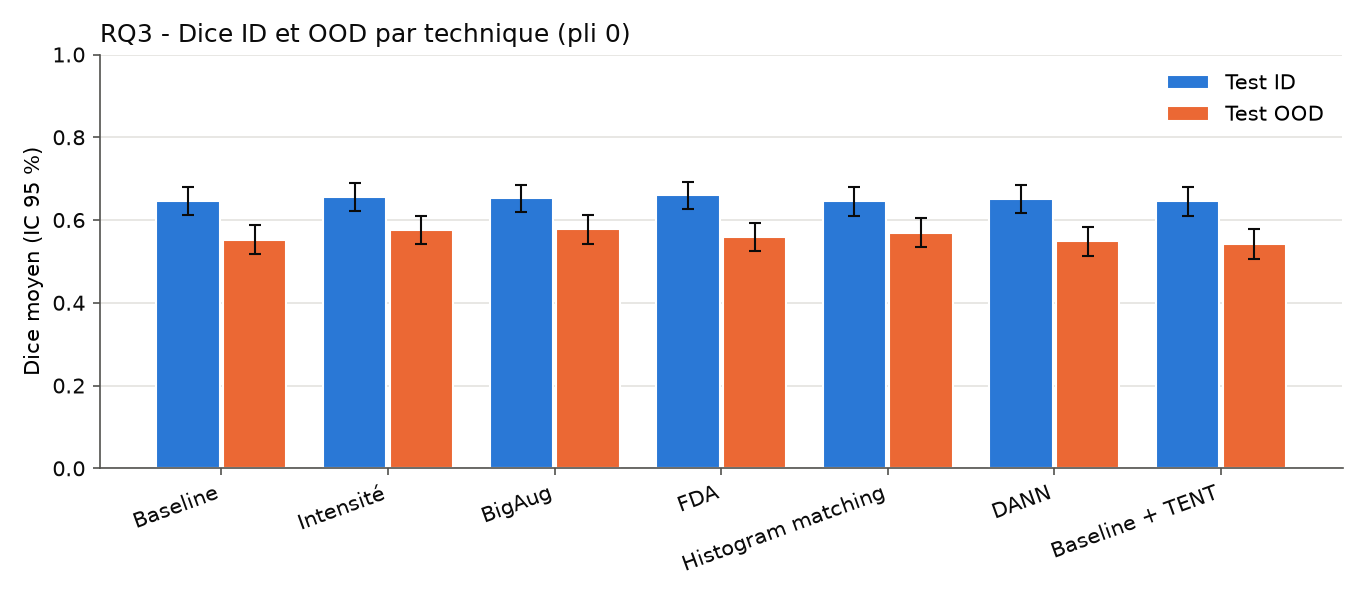
\includegraphics[width=0.8\linewidth]{figures/rq3/rq3_dice_id_ood.png}
  \caption{Dice moyen sur les tests ID et OOD par technique, avec IC à 95~\% (pli~0).}
  \label{fig:rq3-dice-id-ood}
\end{figure}

La figure~\ref{fig:rq3-delta-ood} montre la distribution des différences appariées à la baseline sur le test OOD.
\begin{itemize}
  \item L'augmentation d'intensité est la seule technique qui améliore le Dice OOD de façon significative après correction : $+0{,}024$ [0,008 ; 0,041], $p = 0{,}0014$, $p$ Holm $= 0{,}0068$. Le gain est réparti : 155 sujets sur 252 différences non nulles sont en sa faveur, pour une médiane de $+0{,}006$.
  \item BigAug obtient le même gain moyen ($+0{,}025$ [0,010 ; 0,040]), mais son Wilcoxon ($p = 0{,}035$) n'est plus significatif après correction ($p$ Holm $= 0{,}14$). La différence médiane avec la baseline est quasi nulle ($+0{,}001$ ; 135 sujets en sa faveur sur 250 différences non nulles), et la moyenne est tirée par quelques grands écarts, jusqu'à $+0{,}67$. C'est ce qui explique que le Wilcoxon, fondé sur les rangs, ne passe pas la correction de Holm. Son écart ID $-$ OOD est le plus faible (0,075), mais son IC chevauche celui de la baseline.
  \item FDA a le meilleur Dice ID (0,660), mais son gain sur la baseline n'est significatif après correction ni en ID (Wilcoxon $p = 0{,}012$, $p$ Holm $= 0{,}061$ ; $\Delta$ ID $= +0{,}014$ [$-$0,001 ; 0,029]), ni en OOD ($p = 0{,}32$).
  Avant correction, le Wilcoxon en ID est significatif alors que l'IC bootstrap de $\Delta$ ID contient 0, car les deux ne testent pas la même chose.
  Le Wilcoxon porte sur les rangs des différences appariées : 109 sujets sur 179 différences non nulles sont en faveur de FDA, pour une médiane de $+0{,}005$.
  L'IC porte sur la moyenne, que quelques grandes différences dans les deux sens (jusqu'à $-0{,}32$) rendent plus variable.
  \item Histogram matching améliore le Dice OOD en moyenne ($+0{,}017$ [0,001 ; 0,034]), mais pas de façon significative ($p = 0{,}24$, $p$ Holm $= 0{,}49$). L'IC bootstrap de $\Delta$ OOD exclut tout juste 0 alors que le Wilcoxon n'est pas significatif, pour la même raison que FDA en ID : l'IC porte sur la moyenne, tirée par quelques grands écarts (jusqu'à $+0{,}84$), et le Wilcoxon sur les rangs, avec une médiane nulle (125 sujets en sa faveur, 125 en sa défaveur). Son écart ID $-$ OOD (0,077) est proche de celui de BigAug.
  \item DANN ne se distingue de la baseline ni en ID ($p = 0{,}45$) ni en OOD ($p = 0{,}13$).
  \item TENT abaisse le Dice OOD de 0,011 [0,006 ; 0,016]. L'effet est petit mais systématique ($p < 10^{-4}$). En ID, la baisse est de 0,0007 [0,0002 ; 0,0012] ($p = 1{,}7 \times 10^{-4}$, $p$ Holm $= 1{,}0 \times 10^{-3}$).
\end{itemize}

\begin{figure}[htbp]
  \centering
  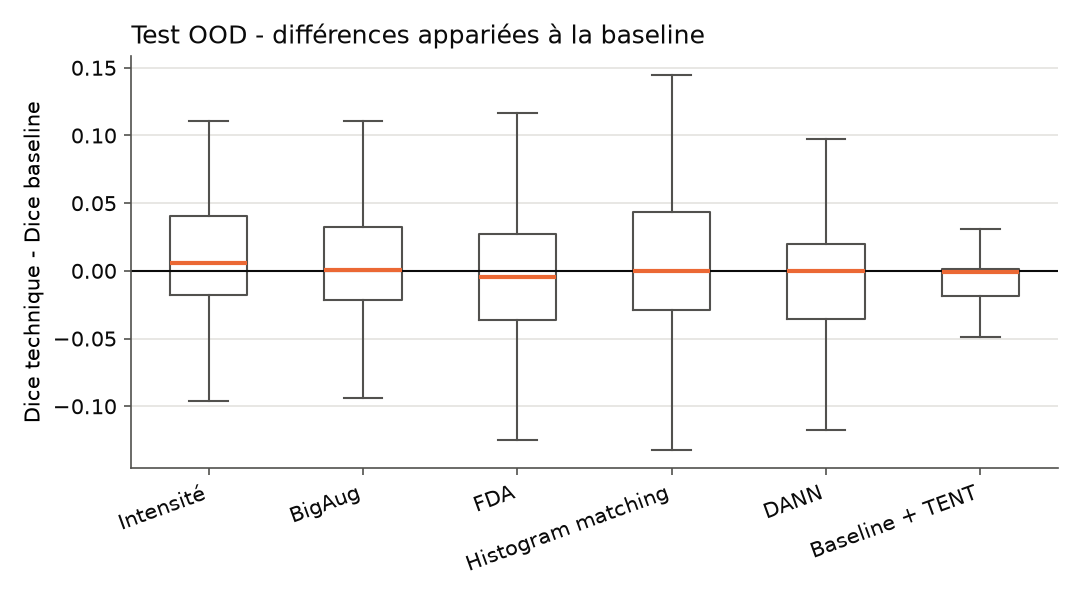
\includegraphics[width=0.8\linewidth]{figures/rq3/rq3_delta_ood.png}
  \caption{Différences appariées de Dice avec la baseline, par sujet, sur le test OOD.}
  \label{fig:rq3-delta-ood}
\end{figure}

\paragraph{BigAug et intensité.}
Le tableau~\ref{tab:rq3-bigaug-intensite} compare directement les deux techniques sur les mêmes sujets (\nolinkurl{adaptation/outputs/rq3/comparaisons.csv}).
Sur le test OOD, la différence moyenne BigAug $-$ intensité vaut $+0{,}001$ [$-0{,}010$ ; 0,012] ($p = 0{,}53$ ; 123 sujets en faveur de BigAug, 128 en faveur de l'intensité).
Sur le test ID, elle vaut $-0{,}003$ [$-0{,}017$ ; 0,011] ($p = 0{,}35$).
Aucun centre OOD ne les sépare : les différences vont de $-0{,}011$ (R034) à $+0{,}006$ (R008), toutes avec $p \geq 0{,}32$.
Les deux techniques sont donc équivalentes en Dice à la précision de cette étude.
Elles diffèrent sur deux points secondaires.
L'entraînement de BigAug dure 8,1~h contre 5,0~h pour l'intensité (\nolinkurl{adaptation/outputs/rq3/entrainement.csv}).
Le F1 des lésions OOD est plus élevé avec l'intensité qu'avec BigAug (0,450 contre 0,420), mais les deux restent sous la baseline (0,477, tableau~\ref{tab:rq3-secondaires}) : ce n'est qu'un avantage relatif face à BigAug.

\begin{table}[htbp]
  \centering
  \caption{Comparaison directe BigAug $-$ intensité par centre OOD (sujets appariés). Source : \texttt{comparaisons\_par\_centre.csv}.}
  \label{tab:rq3-bigaug-intensite}
  \small
  \setlength{\tabcolsep}{4pt}
  \begin{tabular}{lcccccc}
    \toprule
    Centre & n & Dice BigAug & Dice intensité & $\Delta$ moyen & \makecell{Sujets\\BigAug > / < intensité} & $p$ Wilcoxon \\
    \midrule
    R008 & 7 & 0,006 & 0,000 & +0,006 & 1 / 0 & 1 \\
    R028 & 26 & 0,652 & 0,649 & +0,003 & 16 / 10 & 0,50 \\
    R031 & 37 & 0,663 & 0,672 & $-$0,009 & 15 / 22 & 0,32 \\
    R034 & 24 & 0,642 & 0,653 & $-$0,011 & 11 / 12 & 0,76 \\
    R053 & 4 & 0,195 & 0,197 & $-$0,002 & 1 / 1 & 1 \\
    SOOP & 167 & 0,571 & 0,567 & +0,004 & 79 / 83 & 0,60 \\
    \midrule
    Total OOD & 265 & 0,577 & 0,577 & +0,001 & 123 / 128 & 0,53 \\
    \bottomrule
  \end{tabular}
\end{table}

\paragraph{Histogram matching et intensité.}
Le tableau~\ref{tab:rq3-hm-intensite} compare de la même façon histogram matching et intensité.
Sur le test OOD, la différence moyenne histogram matching $-$ intensité vaut $-0{,}007$ [$-0{,}023$ ; 0,009] ($p = 0{,}062$ ; 110 sujets en faveur d'histogram matching, 142 en faveur de l'intensité).
Sur le test ID, elle vaut $-0{,}010$ [$-0{,}025$ ; 0,005] ($p = 0{,}35$).
Le seul écart net par centre concerne R031 : $-0{,}059$ ($p = 0{,}0018$ ; 10 sujets contre 27), qui reste sous 0,05 après une correction de Bonferroni sur les six centres.
Histogram matching a en revanche un F1 des lésions OOD supérieur à celui de la baseline (0,486 contre 0,477) et le plus faible écart absolu de volume de toutes les techniques (9,1~ml, tableau~\ref{tab:rq3-secondaires}).

\begin{table}[htbp]
  \centering
  \caption{Comparaison directe histogram matching $-$ intensité par centre OOD (sujets appariés). HM : histogram matching. Source : \texttt{comparaisons\_par\_centre.csv}.}
  \label{tab:rq3-hm-intensite}
  \small
  \setlength{\tabcolsep}{4pt}
  \begin{tabular}{lcccccc}
    \toprule
    Centre & n & Dice HM & Dice intensité & $\Delta$ moyen & \makecell{Sujets\\HM > / < intensité} & $p$ Wilcoxon \\
    \midrule
    R008 & 7 & 0,019 & 0,000 & +0,019 & 1 / 0 & 1 \\
    R028 & 26 & 0,659 & 0,649 & +0,010 & 16 / 9 & 0,23 \\
    R031 & 37 & 0,614 & 0,672 & $-$0,059 & 10 / 27 & 0,0018 \\
    R034 & 24 & 0,648 & 0,653 & $-$0,005 & 14 / 9 & 0,41 \\
    R053 & 4 & 0,237 & 0,197 & +0,040 & 1 / 1 & 1 \\
    SOOP & 167 & 0,566 & 0,567 & 0,000 & 68 / 96 & 0,11 \\
    \midrule
    Total OOD & 265 & 0,570 & 0,577 & $-$0,007 & 110 / 142 & 0,062 \\
    \bottomrule
  \end{tabular}
\end{table}

\paragraph{Lecture des résultats négatifs.}
Les résultats de DANN et de TENT ne sont pas des défaillances techniques. La run DANN est allée à son terme, avec un contrôle de reprise validé (section~\ref{sec:rq3-limites}). TENT a été appliqué au modèle baseline sur les mêmes sujets. Les deux sont évalués comme les autres techniques.
Pour DANN, l'alignement des caractéristiques entre 39 centres n'apporte rien de mesurable.
Une explication compatible avec nos données est que les échecs OOD dépendent surtout de la taille et du contraste des lésions (section~\ref{sec:rq3-echecs}), deux facteurs que l'alignement des centres ne traite pas.
Pour TENT, la minimisation de l'entropie rend les prédictions plus tranchées sans étiquettes. La baisse touche surtout les lésions de plus de 50~ml (0,71 contre 0,74, tableau~\ref{tab:rq3-taille}).

\paragraph{Métriques secondaires.}
Elles ne suivent pas toujours le Dice (tableau~\ref{tab:rq3-secondaires}).
Le F1 des lésions OOD baisse avec l'intensité (0,450 contre 0,477), BigAug (0,420), FDA et DANN (0,366 et 0,367) ; il augmente avec histogram matching (0,486) et TENT (0,495).
L'écart absolu de volume baisse surtout avec histogram matching (9,1~ml contre 11,1~ml), puis avec l'intensité (10,0~ml) et BigAug (10,9~ml).

\begin{table}[htbp]
  \centering
  \caption{Métriques secondaires moyennes sur le test OOD (\texttt{tableau\_rq3.csv}).}
  \label{tab:rq3-secondaires}
  \begin{tabular}{lccc}
    \toprule
    Technique & F1 des lésions & HD95 (mm) & Écart absolu de volume (ml) \\
    \midrule
    Baseline & 0,477 & 24,9 & 11,1 \\
    Intensité & 0,450 & 25,5 & 10,0 \\
    BigAug & 0,420 & 25,4 & 10,9 \\
    FDA & 0,366 & 26,1 & 13,3 \\
    Histogram matching & 0,486 & 24,9 & 9,1 \\
    DANN & 0,367 & 27,2 & 12,1 \\
    Baseline + TENT & 0,495 & 25,9 & 12,1 \\
    \bottomrule
  \end{tabular}
\end{table}

\paragraph{Validation et test.}
Les meilleurs Dice de validation vont de 0,427 à 0,443 (\nolinkurl{adaptation/outputs/rq3/entrainement.csv}). La validation ne départage donc pas les techniques.
Le Dice de validation (environ 0,43) est plus bas que celui du test ID (0,646) pour deux raisons.
La validation porte sur neuf centres non vus.
Ses lésions sont aussi plus petites : médiane de 1,26~ml et 43~\% sous 1~ml, contre 7,56~ml et 18~\% au test ID (volumes \texttt{lesion\_ml} des fichiers \texttt{qc.json}).

\section{Analyse des échecs}
\label{sec:rq3-echecs}

Les tableaux détaillés de cette section sont produits par le script \nolinkurl{adaptation/analyse_echecs.py}.
Ils se trouvent dans le dossier \nolinkurl{adaptation/outputs/rq3/echecs/}.

\subsection{Dice par centre OOD}

Le tableau~\ref{tab:rq3-centres} et la figure~\ref{fig:rq3-dice-centre} donnent le Dice moyen par centre.
Le contraste T1 est la différence entre le z-score moyen de la lésion et celui d'un anneau de 1 à 4~mm autour d'elle. Une lésion chronique est hypo-intense, et son contraste est négatif.

\begin{table}[htbp]
  \centering
  \caption{Centres OOD, rangés par distance décroissante au reste des centres. Vol. : volume médian des lésions ; J : jours après l'AVC (médiane) ; W1 : distance de Wasserstein ; Base. : baseline ; Int. : intensité ; HM : histogram matching ; TENT : baseline + TENT. Source : \texttt{par\_centre\_ood.csv}.}
  \label{tab:rq3-centres}
  \small
  \setlength{\tabcolsep}{3pt}
  \begin{tabular}{lcccccccccccc}
    \toprule
    & & & & & & \multicolumn{7}{c}{Dice moyen} \\
    \cmidrule(lr){7-13}
    Centre & \makecell{Sujets\\(lésion)} & \makecell{Vol.\\(ml)} & J & W1 & Contraste & Base. & Int. & BigAug & FDA & HM & DANN & TENT \\
    \midrule
    R008 & 7 (7) & 0,95 & 1 & 0,216 & $-$0,17 & 0,00 & 0,00 & 0,01 & 0,00 & 0,02 & 0,00 & 0,00 \\
    R031 & 37 (37) & 6,74 & 138 & 0,164 & $-$0,98 & 0,62 & 0,67 & 0,66 & 0,65 & 0,61 & 0,63 & 0,62 \\
    R028 & 26 (26) & 4,94 & 576 & 0,157 & $-$0,82 & 0,66 & 0,65 & 0,65 & 0,64 & 0,66 & 0,65 & 0,66 \\
    SOOP & 169 (167) & 22,75 & -- & 0,023 & $-$0,69 & 0,54 & 0,57 & 0,57 & 0,54 & 0,57 & 0,53 & 0,52 \\
    R053 & 5 (4) & 0,81 & 25 & 0,020 & $-$0,50 & 0,20 & 0,20 & 0,20 & 0,22 & 0,24 & 0,25 & 0,20 \\
    R034 & 24 (24) & 2,38 & 1\,506 & 0,014 & $-$0,64 & 0,63 & 0,65 & 0,64 & 0,66 & 0,65 & 0,64 & 0,63 \\
    \bottomrule
  \end{tabular}
\end{table}

\begin{figure}[htbp]
  \centering
  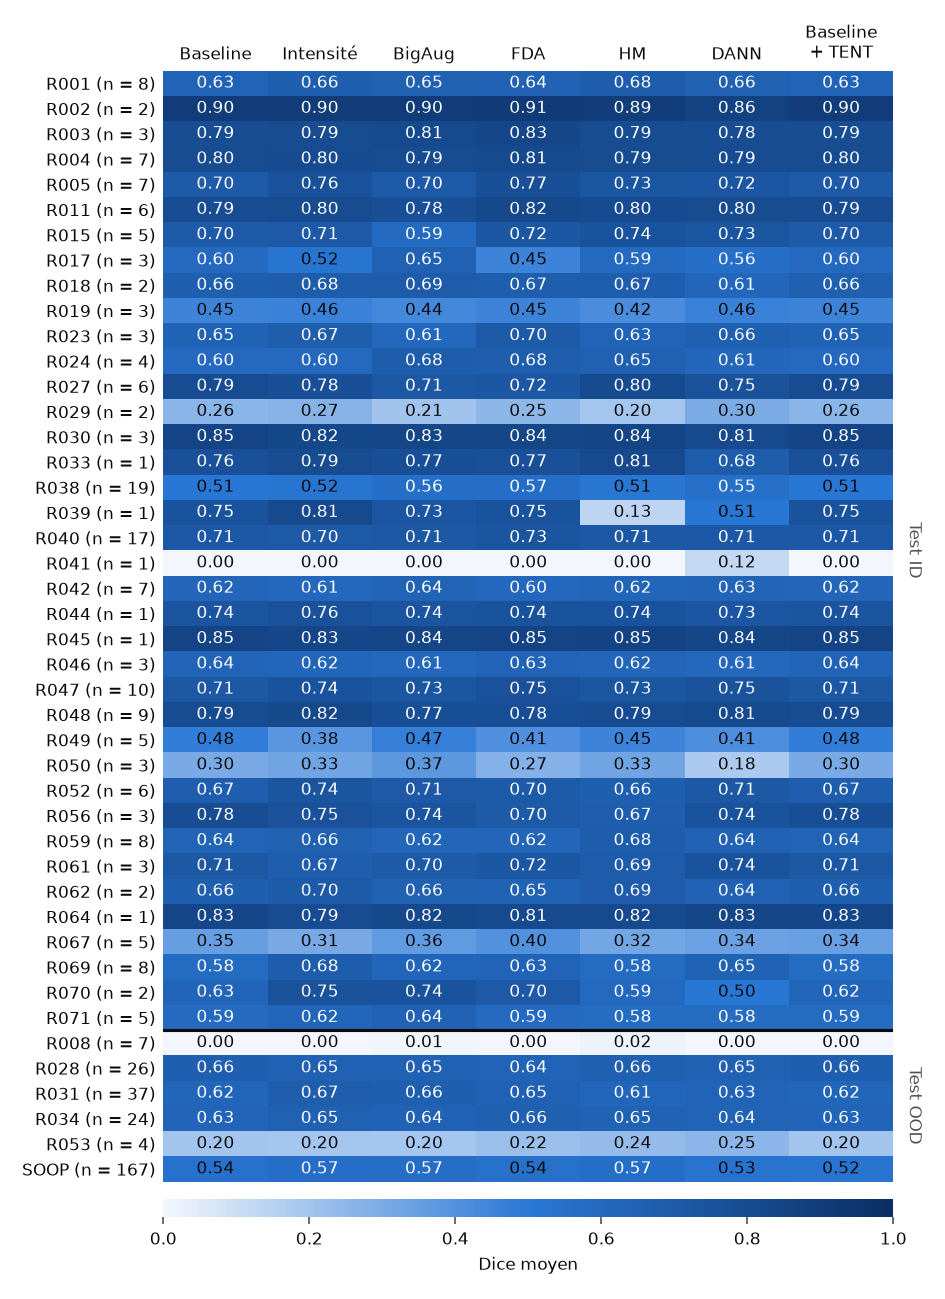
\includegraphics[width=\linewidth]{figures/rq3/rq3_dice_par_centre.png}
  \caption{Dice moyen par centre de test (ID et OOD) et par technique. HM : histogram matching.}
  \label{fig:rq3-dice-centre}
\end{figure}

\subsection{Taille des lésions}

La taille est le facteur le plus net.
Sur les 265 sujets OOD, la corrélation de Spearman entre le volume de la lésion et le Dice (modèle intensité) vaut $\rho = 0{,}53$ ($p < 10^{-4}$).
Le tableau~\ref{tab:rq3-taille} et la figure~\ref{fig:rq3-dice-taille} montrent que toutes les techniques suivent le même profil.
L'intensité gagne surtout entre 1 et 50~ml (0,50 et 0,67 contre 0,46 et 0,64 pour la baseline). BigAug gagne surtout au-dessus de 10~ml (0,68 et 0,77 contre 0,64 et 0,74).

\begin{table}[htbp]
  \centering
  \caption{Dice moyen par volume de lésion sur le test OOD (Dice ID entre parenthèses). L'adaptation continue porte sur un sous-ensemble des sujets.}
  \label{tab:rq3-taille}
  \small
  \begin{tabular}{lcccc}
    \toprule
    Technique & $< 1$~ml & 1--10~ml & 10--50~ml & $\geq 50$~ml \\
    \midrule
    Sujets OOD (ID) & 41 (34) & 86 (65) & 80 (48) & 58 (38) \\
    \midrule
    Baseline & 0,31 (0,48) & 0,46 (0,58) & 0,64 (0,71) & 0,74 (0,83) \\
    Intensité & 0,33 (0,46) & 0,50 (0,59) & 0,67 (0,74) & 0,74 (0,83) \\
    BigAug & 0,32 (0,43) & 0,48 (0,59) & 0,68 (0,75) & 0,77 (0,83) \\
    FDA & 0,30 (0,44) & 0,46 (0,61) & 0,66 (0,74) & 0,75 (0,84) \\
    Histogram matching & 0,33 (0,49) & 0,49 (0,58) & 0,66 (0,71) & 0,74 (0,83) \\
    DANN & 0,29 (0,46) & 0,45 (0,58) & 0,63 (0,73) & 0,75 (0,83) \\
    Baseline + TENT & 0,32 (0,48) & 0,46 (0,58) & 0,62 (0,71) & 0,71 (0,82) \\
    Continue (contrôlée) & 0,35 & 0,48 & 0,60 & 0,81 \\
    \bottomrule
  \end{tabular}
\end{table}

\begin{figure}[htbp]
  \centering
  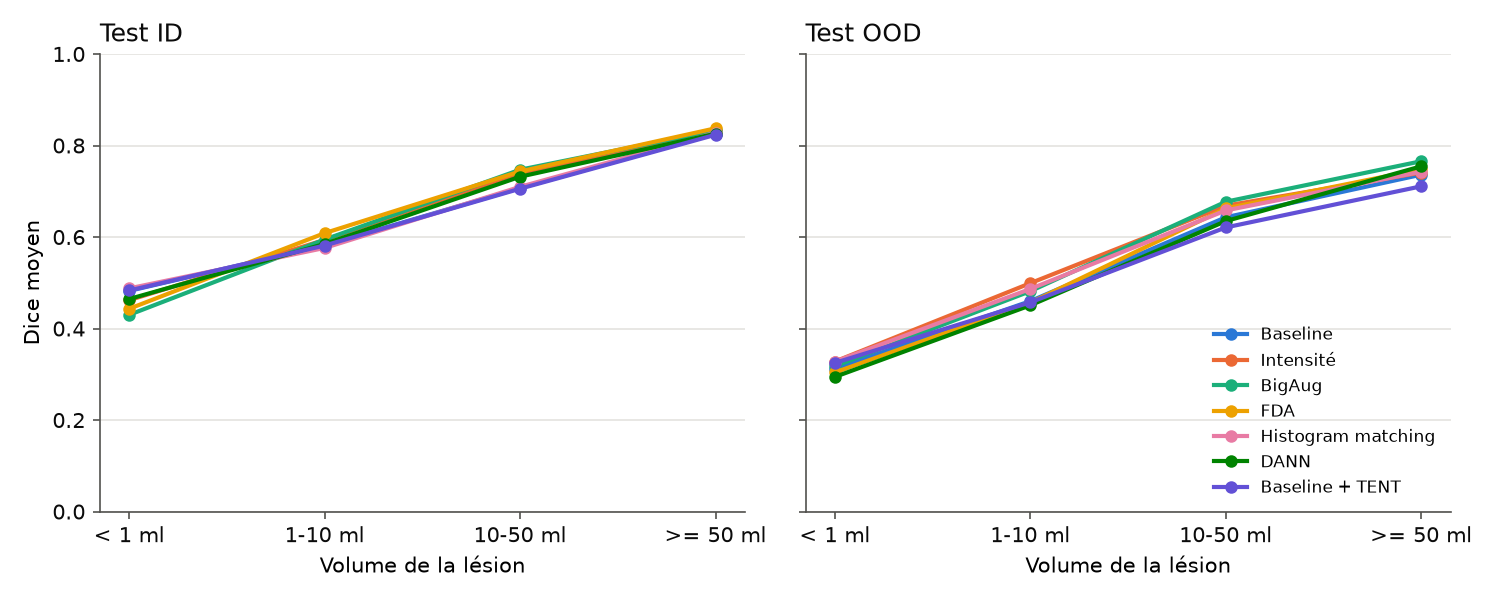
\includegraphics[width=\linewidth]{figures/rq3/rq3_dice_par_taille.png}
  \caption{Dice moyen par classe de volume de lésion, sur les tests ID (à gauche) et OOD (à droite).}
  \label{fig:rq3-dice-taille}
\end{figure}

La figure~\ref{fig:rq3-echecs-taille} reprend le test OOD en y ajoutant l'adaptation continue contrôlée.

\begin{figure}[htbp]
  \centering
  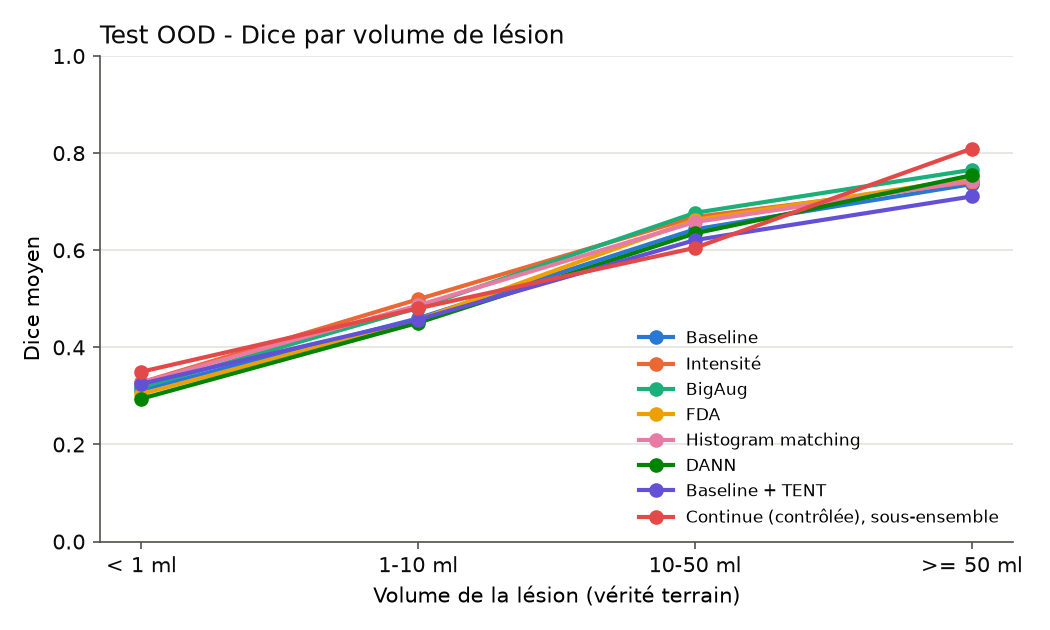
\includegraphics[width=0.8\linewidth]{figures/rq3/rq3_echecs_dice_par_taille.png}
  \caption{Dice moyen par volume de lésion sur le test OOD, avec l'adaptation continue contrôlée (sous-ensemble préquentiel).}
  \label{fig:rq3-echecs-taille}
\end{figure}

\subsection{Centre R008}

Toutes les techniques obtiennent un Dice nul ou presque sur R008. Le Dice moyen de BigAug est de 0,006 sur le centre ; un seul sujet est non nul, à 0,04 (tableau~\ref{tab:rq3-bigaug-intensite} ; moyenne arrondie à 0,01 dans le tableau~\ref{tab:rq3-centres}). Celui d'histogram matching est de 0,019, avec un seul sujet non nul, à 0,13 (tableau~\ref{tab:rq3-hm-intensite}). Le détail par sujet est dans \nolinkurl{zoom_R008_R053.csv}.
\begin{itemize}
  \item Six sujets sur sept sont imagés au premier jour après l'AVC. Leurs lésions font de 0,1 à 4,1~ml.
  \item Les lésions sont peu visibles en T1 : contraste médian de $-0{,}17$, contre $-0{,}50$ à $-0{,}98$ dans les autres centres OOD.
  \item Les intensités sont atypiques : 1,1 à 1,7~\% des voxels du cerveau dépassent $z = 3$, contre 0,003~\% en médiane chez les autres sujets OOD (\nolinkurl{contraste_lesions.csv}).
  \item Le modèle prédit de 0,4 à 33,6~ml répartis en nombreuses composantes, pour une différence du nombre de lésions de 9 à 67.
  \item À l'examen des coupes, vaisseaux, sinus et dure-mère apparaissent hyperintenses.
\end{itemize}
% Les coupes de R008 (figures/rq3/rq3_echecs_coupes_R008.png) ne sont pas incluses :
% ce sont des images ATLAS, non versionnées ; elles se régénèrent avec adaptation/analyse_echecs.py.

\emph{Hypothèse.} La séquence T1 de R008 aurait été acquise après injection de gadolinium, en phase aiguë.
La lésion n'y aurait pas encore le contraste T1 des lésions chroniques, majoritaires à l'entraînement.
Le décalage serait alors à la fois d'acquisition et de stade clinique.
Cette hypothèse reste à vérifier sur le protocole d'acquisition de R008 et sur l'écart entre la date de l'IRM et celle de l'annotation.

\subsection{Centre R053}

Le Dice moyen de R053 est de 0,20 sur quatre sujets ; un cinquième sujet a un masque vide et est exclu du Dice.
Deux lésions minuscules (0,13 et 0,015~ml) ont un Dice de 0. Les deux autres (1,5 et 2,6~ml) obtiennent 0,27 et 0,52.
Les intensités sont dans la norme (99\textsuperscript{e} centile du z-score proche de 1,8) et le contraste vaut $-0{,}50$.
L'échec s'explique par la taille des lésions, pas par un décalage d'intensité. Avec quatre sujets, la moyenne du centre est très instable.

\subsection{Distance de domaine}

La distance de Wasserstein entre histogrammes d'intensité (\nolinkurl{analysis/center_distance.py}, référence = tous les autres centres) ne prédit pas le Dice dans nos runs (\nolinkurl{spearman.csv}).
\begin{itemize}
  \item Sur les six centres OOD, $\rho$ va de $-0{,}43$ à $-0{,}03$ selon la technique ($p$ de 0,40 à 0,96). Avec la MMD, $\rho$ va de $-0{,}37$ à $-0{,}09$.
  \item Sur les 44 centres de test (ID et OOD), $\rho$ va de 0,03 à 0,12 ($p \geq 0{,}44$).
\end{itemize}
La figure~\ref{fig:rq3-distance} en donne deux contre-exemples. R053 est l'un des centres les plus proches (0,020) et l'un des pires. R031 est éloigné (0,164) et parmi les meilleurs.
Six centres offrent une puissance très faible : nous ne concluons pas à l'absence de lien, seulement qu'il n'apparaît pas ici.

\begin{figure}[htbp]
  \centering
  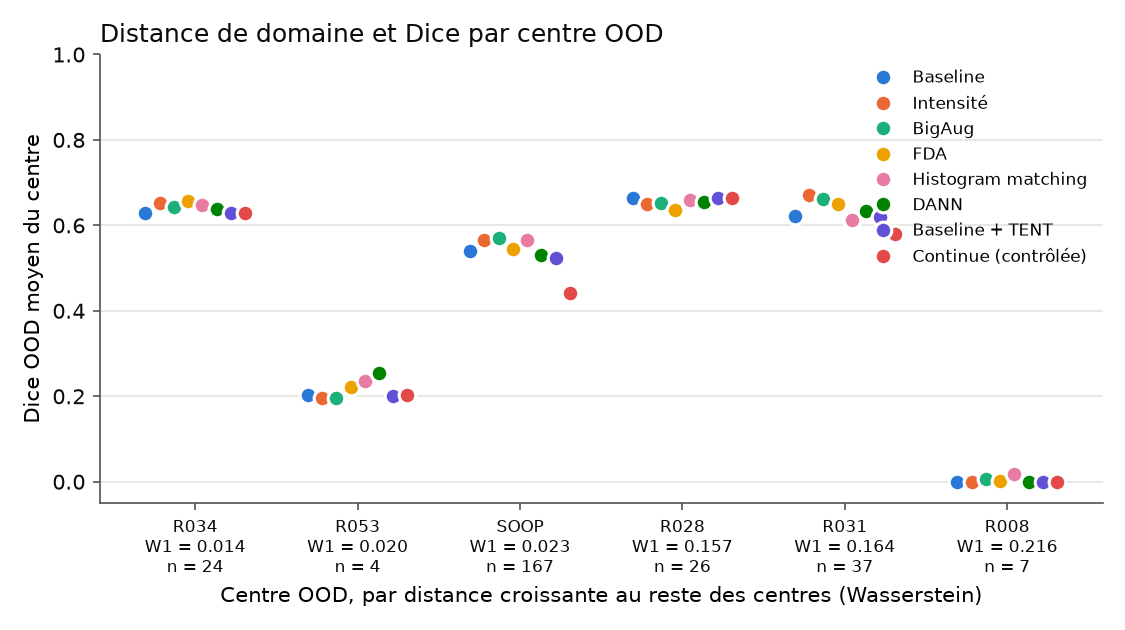
\includegraphics[width=0.8\linewidth]{figures/rq3/rq3_echecs_distance_dice.png}
  \caption{Dice OOD moyen par centre, les centres étant rangés par distance croissante au reste des centres.}
  \label{fig:rq3-distance}
\end{figure}

Au niveau des sujets, le contraste de la lésion n'est que faiblement lié au Dice ($\rho = -0{,}19$, $p = 0{,}001$). La figure~\ref{fig:rq3-contraste} montre ce nuage et place les sujets de R008 et R053.

\begin{figure}[htbp]
  \centering
  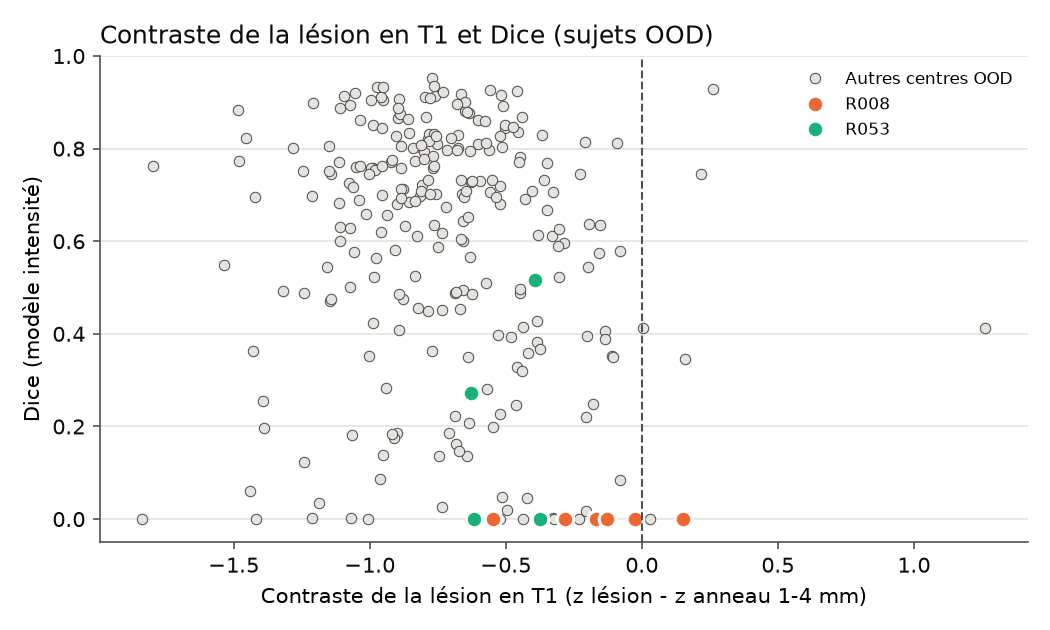
\includegraphics[width=0.8\linewidth]{figures/rq3/rq3_echecs_contraste_dice.png}
  \caption{Contraste T1 de la lésion et Dice (modèle intensité) pour les sujets OOD ; R008 et R053 sont mis en évidence.}
  \label{fig:rq3-contraste}
\end{figure}

\section{Adaptation continue contrôlée}
\label{sec:rq3-continue}

\paragraph{Protocole.}
L'expérience est réalisée par le script \nolinkurl{adaptation/continual.py}.
Ses sorties se trouvent dans le dossier \nolinkurl{adaptation/outputs/rq3/adaptation_continue/}.
Le modèle baseline reçoit les six centres OOD l'un après l'autre, par lots de quatre sujets : 28 lots, 108 sujets, au plus 24 par centre. Il n'est jamais réinitialisé.
L'évaluation est préquentielle : chaque lot est d'abord noté (Dice), puis utilisé pour l'adaptation, sans étiquettes.
Quatre stratégies sont comparées sur les mêmes lots :
\begin{itemize}
  \item \texttt{fige} : le modèle reste inchangé ;
  \item \texttt{auto\_apprentissage} : pseudo-étiquettes, tous les poids sont mis à jour ;
  \item \texttt{tent} : TENT appliqué en continu ;
  \item \texttt{controlee} : TENT dans un modèle candidat, promu seulement si trois conditions sont réunies. (1) La distance du lot dépasse un seuil calibré sur la source (0,077). (2) L'entropie baisse sur des patches neufs. (3) Le Dice sur un jeu de garde étiqueté de la source ne baisse pas de plus de 0,01. Cette stratégie rejoue aussi des exemples des centres déjà vus et des patches de la source.
\end{itemize}
L'oubli est mesuré après chaque centre, par le Dice sur 16 sujets fixes du test ID et sur les premiers sujets des centres OOD déjà vus.

\paragraph{Résultats.}
Le tableau~\ref{tab:rq3-continue} résume les quatre stratégies (\nolinkurl{resume.json}, \nolinkurl{oubli.csv}).

\begin{table}[htbp]
  \centering
  \caption{Adaptation continue sur les six centres OOD : Dice préquentiel et oubli.}
  \label{tab:rq3-continue}
  \small
  \begin{tabular}{lcccc}
    \toprule
    Stratégie & \makecell{Dice\\préquentiel} & \makecell{Dice ID\\(début $\rightarrow$ fin)} & Oubli ID & \makecell{Oubli OOD\\moyen} \\
    \midrule
    Figé & 0,528 & 0,635 $\rightarrow$ 0,635 & 0,000 & 0,000 \\
    Auto-apprentissage & 0,486 & 0,635 $\rightarrow$ 0,583 & 0,052 & 0,033 \\
    TENT continu & 0,526 & 0,635 $\rightarrow$ 0,632 & 0,002 & 0,000 \\
    Contrôlée & 0,527 & 0,635 $\rightarrow$ 0,634 & 0,001 & 0,000 \\
    \bottomrule
  \end{tabular}
\end{table}

Les décisions lot par lot sont dans \nolinkurl{decisions.csv}.
\begin{itemize}
  \item \textbf{Détection.} Un décalage est détecté sur 15 lots sur 28 : tous ceux de R008, R028 et R031, et un lot sur six de SOOP. Il n'est jamais détecté sur R034 ni R053, les centres les plus proches de la source.
  \item \textbf{Promotions.} Douze candidats sont promus : deux pour R008, six pour R028, trois pour R031 et un pour SOOP. Trois candidats de R031 sont refusés parce que leur entropie augmente.
  \item \textbf{Oubli.} La stratégie contrôlée évite l'oubli de l'auto-apprentissage (0,001 contre 0,052 sur le test ID).
  \item \textbf{Gain.} Elle n'améliore pas le Dice par rapport au modèle figé (0,527 contre 0,528).
\end{itemize}

\paragraph{Lecture du résultat.}
L'absence de gain s'explique par la nature des décalages détectés.
R028 et R031 sont déjà bien segmentés par le modèle figé (0,66 et 0,58 en préquentiel).
Sur R008, le problème tient au contraste des lésions (section~\ref{sec:rq3-echecs}), qu'une adaptation des normalisations ne peut pas créer.
Les Dice préquentiels portent sur 108 des 268 sujets OOD ; ils ne se comparent pas directement au tableau~\ref{tab:rq3-resultats}.

\section{Limites}
\label{sec:rq3-limites}

\begin{itemize}
  \item \textbf{Un seul pli et une seule graine.} Les IC traduisent la variabilité des sujets, pas celle de l'entraînement.
  \item \textbf{Reprise de DANN.} La run a été coupée à l'itération 35\,889 et reprise jusqu'à 40\,000. La reprise restaure les poids, l'optimiseur, le taux d'apprentissage, $\lambda$, la position de l'échantillonneur et les états aléatoires des processus de chargement. Le contrôle automatique a validé la première ligne reprise (itération 35\,900, taux $1{,}29 \times 10^{-4}$, $\lambda = 0{,}9771$). Seuls les masques de Dropout du classifieur de centre ne sont pas restaurés. Le meilleur modèle, à l'itération 24\,000, précède de toute façon la coupure.
  \item \textbf{Environnement de DANN.} DANN a été entraînée sur Colab avec torch 2.14.1+cu130 jusqu'à l'itération 35\,889, puis sur Kaggle avec torch 2.11.0+cu130, comme les autres runs. Les deux plateformes utilisent un GPU T4 et CUDA 13.0. Le meilleur modèle (itération 24\,000) vient de la partie Colab. La différence de version de torch peut changer les calculs numériques ; son effet n'a pas été mesuré.
  \item \textbf{Poids de DANN.} Avec un poids de 1, la première run DANN a divergé (perte totale de 10\,508 à l'itération 100 et de 33 millions à l'itération 400). Le poids de 0,1 et la LayerNorm ont été choisis pour la stabilité, sans recherche d'hyperparamètres. Un autre poids pourrait donner un autre résultat.
  \item \textbf{Validation sur des centres non vus.} Ses lésions sont plus petites que celles du test. Elle sert à choisir le checkpoint, mais son Dice (environ 0,43) n'estime pas la performance ID.
  \item \textbf{Diagnostic fp16.} La première baseline, entraînée en fp16, a produit des NaN : des patches entiers donnaient des logits NaN dès l'itération 160 à 180 environ, alors que le fp32 restait stable sur les mêmes lots. Toutes les runs ont été refaites en fp32, environ deux fois plus lentement. La couche qui déborde n'a pas été localisée.
  \item \textbf{Bug de reprise corrigé.} Dans la version du code utilisée pour les runs, la ligne de progression écrasait la file des états aléatoires sauvegardés pour la reprise. Le défaut ne concerne que les reprises, donc uniquement DANN. Il a été corrigé et couvert par un test. Le checkpoint de DANN a été réparé avant la reprise en ne gardant que les quatre derniers états, qui étaient les bons ; les poids n'ont pas changé.
  \item \textbf{Référence de la distance de domaine.} Pour chaque centre, la référence de \nolinkurl{center_distance} regroupe tous les autres centres, OOD compris, et pas seulement les centres d'entraînement du pli~0. La distance mesure donc l'écart au reste du jeu de données, pas exactement l'écart à ce que le modèle a vu.
  \item \textbf{Version du code d'histogram matching.} Cette run a utilisé une version ultérieure du code (\texttt{dbf2f28} au lieu de \texttt{7449c49}), qui ne diffère que par la correction du bug de reprise. Sans DANN ni reprise, les deux versions donnent des poids identiques (vérifié par un court entraînement sur CPU, pour la baseline et l'intensité).
  \item \textbf{Quota GPU.} Avec 30~h par semaine sur Kaggle, aucun autre pli n'a été entraîné, et l'histogram matching a été lancé après les autres techniques.
  \item \textbf{Portée de TENT et de l'adaptation continue.} Les deux ne sont évalués que sur la baseline.
\end{itemize}

\section{Conclusion}
\label{sec:rq3-conclusion}

Sur le pli~0, seule l'augmentation d'intensité améliore le Dice OOD de façon significative après correction : $+0{,}024$ [0,008 ; 0,041], $p$ Holm $= 0{,}0068$ (tableau~\ref{tab:rq3-resultats}).
BigAug atteint le même Dice OOD (0,577), mais son gain n'est pas significatif après correction ($p$ Holm $= 0{,}14$), et la comparaison directe ne sépare pas les deux techniques ($+0{,}001$ [$-0{,}010$ ; 0,012], tableau~\ref{tab:rq3-bigaug-intensite}).
Histogram matching n'est pas significatif non plus ($+0{,}017$, $p$ Holm $= 0{,}49$) ; il reste en dessous de l'intensité en Dice OOD ($-0{,}007$ [$-0{,}023$ ; 0,009]), avec un écart net sur R031 (tableau~\ref{tab:rq3-hm-intensite}).
Aucune technique ne supprime l'écart ID $-$ OOD, qui reste compris entre 0,075 et 0,104.
FDA, DANN et TENT n'améliorent pas le test OOD ; TENT le dégrade légèrement.
L'adaptation continue contrôlée évite l'oubli sans améliorer le Dice (tableau~\ref{tab:rq3-continue}).
L'analyse des échecs montre que les cas les plus difficiles tiennent aux lésions elles-mêmes, petites ou peu contrastées en T1, plutôt qu'à la distance d'intensité entre centres.
Le livrable C8 (\nolinkurl{adaptation/inference.py}) segmente un T1 et renvoie le masque et le volume de la lésion.
Le modèle retenu pour la démonstration est celui de l'intensité.
À Dice égal avec BigAug, ce choix repose d'abord sur son gain significatif après correction, ensuite sur un entraînement plus court (5,0~h contre 8,1~h).
Son F1 des lésions est supérieur à celui de BigAug (0,450 contre 0,420) mais inférieur à celui de la baseline (0,477) : ce n'est qu'un argument relatif face à BigAug.
Histogram matching a le plus faible écart absolu de volume (9,1~ml contre 10,0~ml pour l'intensité) et un F1 des lésions supérieur à celui de la baseline (0,486 contre 0,477).
Il n'a pas été retenu, car son gain en Dice n'est pas significatif et il exigerait d'harmoniser aussi chaque volume à l'inférence, avec l'histogramme de référence de R059.
Ces constats orientent la suite vers la prédiction des cas à risque, en particulier les lésions de moins de 1~ml et les AVC en phase aiguë.
.
% Paquets attendus dans le préambule : babel (french), graphicx, booktabs, makecell, hyperref, float.
% Réglages à mettre dans le préambule du rapport final :
%   \addto\captionsfrench{\def\tablename{Tableau}}   % « Tableau » au lieu de « Table »
%   \hypersetup{hidelinks}                             % liens sans cadre rouge
% Les chemins des figures sont relatifs à la racine du dépôt.
% Citations : docs/rapport/references_rq3.bib, à ajouter à la commande \bibliography du rapport.

\chapter{Généralisation inter-centres (RQ3) et adaptation continue contrôlée}
\label{chap:rq3}

\section{Introduction}
\label{sec:rq3-introduction}

Ce chapitre étudie la robustesse d'un modèle de segmentation des lésions d'AVC face à des centres d'acquisition jamais vus.
La question de recherche RQ3 est la suivante : « Quelles techniques de data augmentation et/ou d'adaptation de domaine réduisent le plus efficacement l'écart de performance entre centres ? »
Nous mesurons cet écart entre des centres vus à l'entraînement (ID) et des centres non vus (OOD).
Nous décrivons d'abord le protocole et les techniques évaluées, puis les résultats et l'analyse des échecs.
Nous présentons ensuite une adaptation continue contrôlée, avant de discuter les limites de l'étude.

\section{Protocole expérimental}
\label{sec:rq3-protocole}

\paragraph{Données.}
Nous utilisons les images T1 d'ATLAS v2.0~\cite{liew2022atlas}, déjà débarrassées du crâne, après le prétraitement S4 de l'équipe : orientation RAS, rééchantillonnage à 1~mm, recadrage sur le cerveau et z-score dans le cerveau (\nolinkurl{preprocessing/week4.py}).
Le découpage est fixé dans \nolinkurl{splits.json}. Le centre R032 est exclu.

\paragraph{Découpage par centre.}
Six centres sont réservés au test OOD : R008, R028, R031, R034, R053 et SOOP.
Ils ont été choisis sur la taille des centres et la distance entre histogrammes d'intensité, sans consulter le Dice (champ \texttt{selection} de \nolinkurl{splits.json}).
Les autres centres sont répartis en cinq plis. Seul le pli~0 a été entraîné. Le tableau~\ref{tab:rq3-donnees} donne les effectifs.

\begin{table}[htbp]
  \centering
  \caption{Effectifs du pli~0.}
  \label{tab:rq3-donnees}
  \begin{tabular}{lrl}
    \toprule
    Ensemble & Sujets & Centres \\
    \midrule
    Entraînement & 733 & 39 \\
    Validation & 183 & 9 centres absents de l'entraînement \\
    Test ID & 185 & centres d'entraînement, sujets non vus \\
    Test OOD & 268 (265 à lésion non vide) & 6 \\
    \bottomrule
  \end{tabular}
\end{table}

Le découpage de \nolinkurl{splits.json} compte 184 sujets de validation.
L'un d'eux, le sujet r065s019 du centre R065, n'a pas de volume prétraité.
Le prétraitement S4 l'a rejeté, car une partie de sa lésion sort du recadrage calculé sur l'image.
Le chargeur l'écarte, et la validation porte donc sur 183 sujets, comme l'indiquent les journaux d'entraînement.
Un de ces 183 sujets a un masque vide : le Dice de validation est calculé sur 182 sujets.

\paragraph{Modèle et entraînement.}
Le réseau est un U-Net~3D de MONAI~\cite{cardoso2022monai} : canaux de 32 à 320, quatre sous-échantillonnages et deux unités résiduelles par niveau.
La normalisation d'instance est affine, ce qu'exige TENT.
L'entraînement utilise des patches de $96^3$ voxels, par lots de quatre patches (deux volumes $\times$ deux patches), dont la moitié est centrée sur la lésion.
Un miroir gauche-droite aléatoire est appliqué à toutes les runs.
La perte combine Dice et entropie croisée.
L'optimiseur AdamW part d'un taux d'apprentissage de $10^{-3}$, avec une décroissance polynomiale (puissance 0,9) et une décroissance des poids de $10^{-5}$.
La norme des gradients est écrêtée à 12.
Toutes les techniques reçoivent le même budget : 40\,000 itérations, graine 2026, calcul en fp32 sur un GPU T4.
Les runs ont été exécutées sur Kaggle (torch 2.11.0+cu130), sauf DANN.
DANN a été entraînée sur Google Colab (GPU T4, torch 2.14.1+cu130) jusqu'à l'itération 35\,889, puis reprise sur Kaggle jusqu'à 40\,000 (section~\ref{sec:rq3-limites}).

\paragraph{Sélection du modèle.}
Le modèle est validé toutes les 2\,000 itérations sur les 183 sujets de validation, en volume entier, par fenêtre glissante de $96^3$ (recouvrement 0,25).
Le checkpoint retenu est celui du meilleur Dice de validation. Il est évalué une seule fois sur les tests ID et OOD.

\paragraph{Métriques.}
Nous rapportons le Dice, la distance de Hausdorff à 95~\% (HD95), l'écart absolu de volume, le F1 des lésions et la différence du nombre de lésions.
Ces métriques sont communes à l'équipe (\nolinkurl{baselines/common.py}).
Le Dice n'est calculé que sur les sujets dont la lésion n'est pas vide.

\paragraph{Tests statistiques.}
Les moyennes sont données avec un intervalle de confiance (IC) à 95~\% par bootstrap percentile (10\,000 tirages).
Pour l'écart ID $-$ OOD, les deux groupes sont rééchantillonnés indépendamment.
Chaque technique est comparée à la baseline par un test des rangs signés de Wilcoxon~\cite{wilcoxon1945}, apparié sur les mêmes sujets.
Une correction de Holm~\cite{holm1979} est appliquée sur l'ensemble des techniques comparées.
La correction porte sur six comparaisons : intensité, BigAug, FDA, histogram matching, DANN et TENT.
BigAug et histogram matching sont aussi comparés directement à l'intensité (différence appariée, IC bootstrap, Wilcoxon), hors correction de Holm : ce sont des comparaisons secondaires avec la technique de référence.

\section{Techniques évaluées}
\label{sec:rq3-techniques}

Toutes les techniques partagent le réseau, les plis, les graines et le budget d'itérations. Seule l'étape propre à chaque technique change (\nolinkurl{adaptation/train.py}, \nolinkurl{generalization/configs/}).

\begin{itemize}
  \item \textbf{Augmentation d'intensité.} Gamma ($p = 0{,}3$) et contraste ($p = 0{,}3$), calibrés sur les seuls sujets d'entraînement ; bruit ($p = 0{,}2$), flou ($p = 0{,}2$), champ de biais ($p = 0{,}3$) et basse résolution ($p = 0{,}25$, jusqu'à 3~mm sur un axe).
  \item \textbf{BigAug}~\cite{zhang2020bigaug}. Flou, netteté, bruit, luminosité, gamma (plage calibrée) et transformation affine (échelle de 0,8 à 1,2, rotation de 20\textdegree), chacun avec $p = 0{,}5$. La déformation élastique est désactivée. Les plages sont adoucies par rapport à l'article pour préserver les petites lésions.
  \item \textbf{FDA} (Fourier Domain Adaptation)~\cite{yang2020fda}. L'amplitude basse fréquence est échangée avec celle d'une image d'un centre d'entraînement de référence (R059 pour le pli~0), avec $\beta$ entre 0,015 et 0,03 et $p = 0{,}5$.
  \item \textbf{DANN} (Domain-Adversarial Neural Network)~\cite{ganin2016dann}. Un classifieur des 39 centres d'entraînement est branché sur la sortie du goulot du réseau : moyenne spatiale, LayerNorm sans paramètres, puis perceptron de 64 unités. Une couche d'inversion du gradient le relie à l'encodeur. Le coefficient $\lambda$ est nul pendant les 2\,000 premières itérations, puis suit la montée proposée par Ganin et al.\ ($\gamma = 5$). La perte du centre a un poids de 0,1.
  \item \textbf{TENT}~\cite{wang2021tent}. Adaptation au test, sans étiquettes, du modèle baseline. Seuls les paramètres affines des normalisations sont modifiés, en minimisant l'entropie des prédictions, centre par centre (Adam, taux de $10^{-4}$, quatre patches par sujet).
  \item \textbf{Histogram matching.} L'histogramme d'intensité du cerveau de chaque volume est ramené vers un histogramme de référence, moyenné sur 20 sujets d'un centre d'entraînement (R059 pour le pli~0). La transformation est déterministe ($p = 1$) et s'applique aussi à la validation et au test. Faute de quota GPU, cette run a été lancée après les autres, avec une version ultérieure du code (section~\ref{sec:rq3-limites}).
\end{itemize}
Fan-Net~\cite{yu2023fannet} n'a pas été implémenté ; FDA en reprend le principe (échange d'amplitude de Fourier) sous une forme plus simple.

\section{Résultats RQ3}
\label{sec:rq3-resultats}

Le tableau~\ref{tab:rq3-resultats} résume les résultats sur 185 sujets ID et 265 sujets OOD (\nolinkurl{adaptation/outputs/rq3/tableau_rq3.md}).

\begin{table}[htbp]
  \centering
  \caption{Dice moyen par technique (pli~0), avec l'IC à 95~\% sous chaque valeur. $\Delta$ OOD : différence appariée à la baseline sur le test OOD ; $p$ : test de Wilcoxon, puis $p$ corrigé par Holm.}
  \label{tab:rq3-resultats}
  \small
  \setlength{\tabcolsep}{4pt}
  \begin{tabular}{lccccc}
    \toprule
    Technique & Dice ID & Dice OOD & \makecell{Écart\\ID $-$ OOD} & $\Delta$ OOD & $p$ OOD \\
    \midrule
    Baseline & \makecell{0,646\\{\footnotesize [0,611 ; 0,680]}} & \makecell{0,553\\{\footnotesize [0,517 ; 0,589]}} & \makecell{0,093\\{\footnotesize [0,044 ; 0,142]}} & -- & -- \\[2pt]
    Intensité & \makecell{0,656\\{\footnotesize [0,621 ; 0,690]}} & \makecell{0,577\\{\footnotesize [0,543 ; 0,611]}} & \makecell{0,080\\{\footnotesize [0,031 ; 0,126]}} & \makecell{+0,024\\{\footnotesize [0,008 ; 0,041]}} & \makecell{0,0014\\{\footnotesize (Holm 0,0068)}} \\[2pt]
    BigAug & \makecell{0,653\\{\footnotesize [0,619 ; 0,686]}} & \makecell{0,577\\{\footnotesize [0,543 ; 0,611]}} & \makecell{0,075\\{\footnotesize [0,028 ; 0,122]}} & \makecell{+0,025\\{\footnotesize [0,010 ; 0,040]}} & \makecell{0,035\\{\footnotesize (Holm 0,14)}} \\[2pt]
    FDA & \makecell{0,660\\{\footnotesize [0,626 ; 0,693]}} & \makecell{0,559\\{\footnotesize [0,524 ; 0,593]}} & \makecell{0,101\\{\footnotesize [0,053 ; 0,148]}} & \makecell{+0,006\\{\footnotesize [$-$0,007 ; 0,020]}} & \makecell{0,32\\{\footnotesize (Holm 0,49)}} \\[2pt]
    \makecell[l]{Histogram\\matching} & \makecell{0,646\\{\footnotesize [0,611 ; 0,681]}} & \makecell{0,570\\{\footnotesize [0,536 ; 0,604]}} & \makecell{0,077\\{\footnotesize [0,027 ; 0,125]}} & \makecell{+0,017\\{\footnotesize [0,001 ; 0,034]}} & \makecell{0,24\\{\footnotesize (Holm 0,49)}} \\[2pt]
    DANN & \makecell{0,650\\{\footnotesize [0,616 ; 0,684]}} & \makecell{0,549\\{\footnotesize [0,513 ; 0,584]}} & \makecell{0,102\\{\footnotesize [0,053 ; 0,150]}} & \makecell{$-$0,004\\{\footnotesize [$-$0,018 ; 0,009]}} & \makecell{0,13\\{\footnotesize (Holm 0,39)}} \\[2pt]
    \makecell[l]{Baseline\\+ TENT} & \makecell{0,645\\{\footnotesize [0,610 ; 0,679]}} & \makecell{0,542\\{\footnotesize [0,506 ; 0,578]}} & \makecell{0,104\\{\footnotesize [0,054 ; 0,153]}} & \makecell{$-$0,011\\{\footnotesize [$-$0,016 ; $-$0,006]}} & \makecell{$< 10^{-4}$\\{\footnotesize (Holm $< 10^{-4}$)}} \\[2pt]
    \bottomrule
  \end{tabular}
\end{table}

La figure~\ref{fig:rq3-dice-id-ood} montre les Dice ID et OOD de chaque technique avec leurs IC.
L'écart entre ID et OOD demeure pour toutes les techniques : il va de 0,075 à 0,104, et aucun IC ne contient 0.

\begin{figure}[htbp]
  \centering
  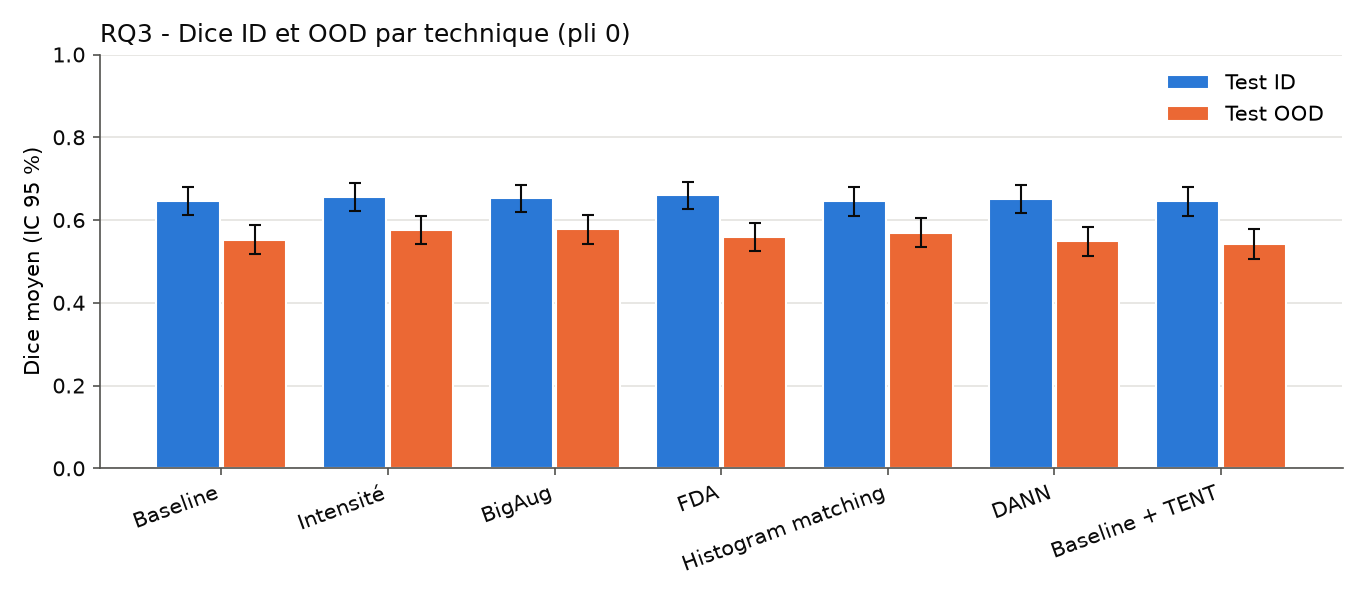
\includegraphics[width=0.8\linewidth]{figures/rq3/rq3_dice_id_ood.png}
  \caption{Dice moyen sur les tests ID et OOD par technique, avec IC à 95~\% (pli~0).}
  \label{fig:rq3-dice-id-ood}
\end{figure}

La figure~\ref{fig:rq3-delta-ood} montre la distribution des différences appariées à la baseline sur le test OOD.
\begin{itemize}
  \item L'augmentation d'intensité est la seule technique qui améliore le Dice OOD de façon significative après correction : $+0{,}024$ [0,008 ; 0,041], $p = 0{,}0014$, $p$ Holm $= 0{,}0068$. Le gain est réparti : 155 sujets sur 252 différences non nulles sont en sa faveur, pour une médiane de $+0{,}006$.
  \item BigAug obtient le même gain moyen ($+0{,}025$ [0,010 ; 0,040]), mais son Wilcoxon ($p = 0{,}035$) n'est plus significatif après correction ($p$ Holm $= 0{,}14$). La différence médiane avec la baseline est quasi nulle ($+0{,}001$ ; 135 sujets en sa faveur sur 250 différences non nulles), et la moyenne est tirée par quelques grands écarts, jusqu'à $+0{,}67$. C'est ce qui explique que le Wilcoxon, fondé sur les rangs, ne passe pas la correction de Holm. Son écart ID $-$ OOD est le plus faible (0,075), mais son IC chevauche celui de la baseline.
  \item FDA a le meilleur Dice ID (0,660), mais son gain sur la baseline n'est significatif après correction ni en ID (Wilcoxon $p = 0{,}012$, $p$ Holm $= 0{,}061$ ; $\Delta$ ID $= +0{,}014$ [$-$0,001 ; 0,029]), ni en OOD ($p = 0{,}32$).
  Avant correction, le Wilcoxon en ID est significatif alors que l'IC bootstrap de $\Delta$ ID contient 0, car les deux ne testent pas la même chose.
  Le Wilcoxon porte sur les rangs des différences appariées : 109 sujets sur 179 différences non nulles sont en faveur de FDA, pour une médiane de $+0{,}005$.
  L'IC porte sur la moyenne, que quelques grandes différences dans les deux sens (jusqu'à $-0{,}32$) rendent plus variable.
  \item Histogram matching améliore le Dice OOD en moyenne ($+0{,}017$ [0,001 ; 0,034]), mais pas de façon significative ($p = 0{,}24$, $p$ Holm $= 0{,}49$). L'IC bootstrap de $\Delta$ OOD exclut tout juste 0 alors que le Wilcoxon n'est pas significatif, pour la même raison que FDA en ID : l'IC porte sur la moyenne, tirée par quelques grands écarts (jusqu'à $+0{,}84$), et le Wilcoxon sur les rangs, avec une médiane nulle (125 sujets en sa faveur, 125 en sa défaveur). Son écart ID $-$ OOD (0,077) est proche de celui de BigAug.
  \item DANN ne se distingue de la baseline ni en ID ($p = 0{,}45$) ni en OOD ($p = 0{,}13$).
  \item TENT abaisse le Dice OOD de 0,011 [0,006 ; 0,016]. L'effet est petit mais systématique ($p < 10^{-4}$). En ID, la baisse est de 0,0007 [0,0002 ; 0,0012] ($p = 1{,}7 \times 10^{-4}$, $p$ Holm $= 1{,}0 \times 10^{-3}$).
\end{itemize}

\begin{figure}[htbp]
  \centering
  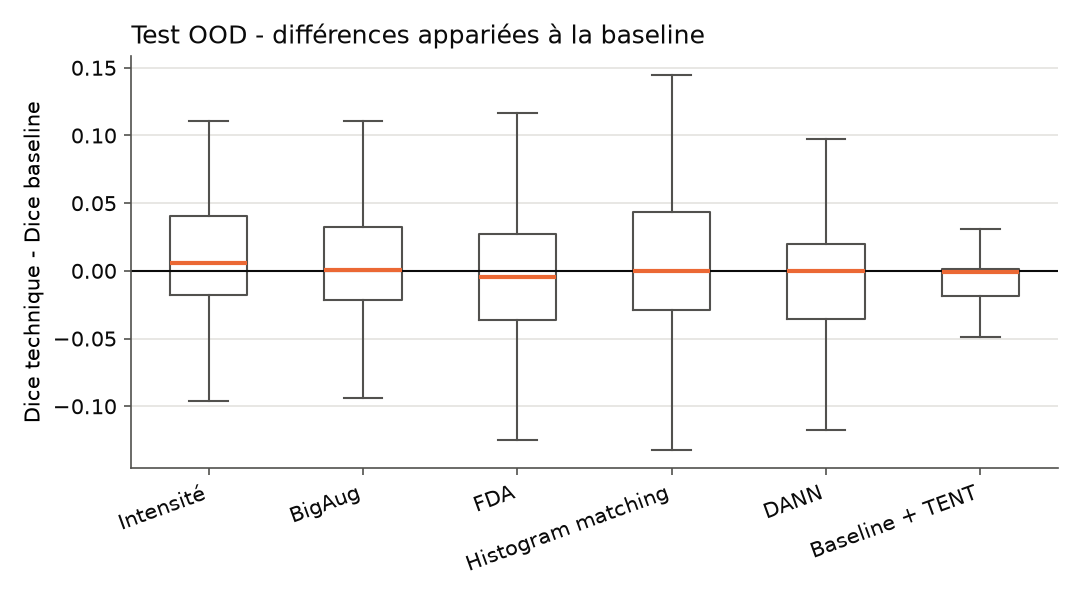
\includegraphics[width=0.8\linewidth]{figures/rq3/rq3_delta_ood.png}
  \caption{Différences appariées de Dice avec la baseline, par sujet, sur le test OOD.}
  \label{fig:rq3-delta-ood}
\end{figure}

\paragraph{BigAug et intensité.}
Le tableau~\ref{tab:rq3-bigaug-intensite} compare directement les deux techniques sur les mêmes sujets (\nolinkurl{adaptation/outputs/rq3/comparaisons.csv}).
Sur le test OOD, la différence moyenne BigAug $-$ intensité vaut $+0{,}001$ [$-0{,}010$ ; 0,012] ($p = 0{,}53$ ; 123 sujets en faveur de BigAug, 128 en faveur de l'intensité).
Sur le test ID, elle vaut $-0{,}003$ [$-0{,}017$ ; 0,011] ($p = 0{,}35$).
Aucun centre OOD ne les sépare : les différences vont de $-0{,}011$ (R034) à $+0{,}006$ (R008), toutes avec $p \geq 0{,}32$.
Les deux techniques sont donc équivalentes en Dice à la précision de cette étude.
Elles diffèrent sur deux points secondaires.
L'entraînement de BigAug dure 8,1~h contre 5,0~h pour l'intensité (\nolinkurl{adaptation/outputs/rq3/entrainement.csv}).
Le F1 des lésions OOD est plus élevé avec l'intensité qu'avec BigAug (0,450 contre 0,420), mais les deux restent sous la baseline (0,477, tableau~\ref{tab:rq3-secondaires}) : ce n'est qu'un avantage relatif face à BigAug.

\begin{table}[htbp]
  \centering
  \caption{Comparaison directe BigAug $-$ intensité par centre OOD (sujets appariés). Source : \texttt{comparaisons\_par\_centre.csv}.}
  \label{tab:rq3-bigaug-intensite}
  \small
  \setlength{\tabcolsep}{4pt}
  \begin{tabular}{lcccccc}
    \toprule
    Centre & n & Dice BigAug & Dice intensité & $\Delta$ moyen & \makecell{Sujets\\BigAug > / < intensité} & $p$ Wilcoxon \\
    \midrule
    R008 & 7 & 0,006 & 0,000 & +0,006 & 1 / 0 & 1 \\
    R028 & 26 & 0,652 & 0,649 & +0,003 & 16 / 10 & 0,50 \\
    R031 & 37 & 0,663 & 0,672 & $-$0,009 & 15 / 22 & 0,32 \\
    R034 & 24 & 0,642 & 0,653 & $-$0,011 & 11 / 12 & 0,76 \\
    R053 & 4 & 0,195 & 0,197 & $-$0,002 & 1 / 1 & 1 \\
    SOOP & 167 & 0,571 & 0,567 & +0,004 & 79 / 83 & 0,60 \\
    \midrule
    Total OOD & 265 & 0,577 & 0,577 & +0,001 & 123 / 128 & 0,53 \\
    \bottomrule
  \end{tabular}
\end{table}

\paragraph{Histogram matching et intensité.}
Le tableau~\ref{tab:rq3-hm-intensite} compare de la même façon histogram matching et intensité.
Sur le test OOD, la différence moyenne histogram matching $-$ intensité vaut $-0{,}007$ [$-0{,}023$ ; 0,009] ($p = 0{,}062$ ; 110 sujets en faveur d'histogram matching, 142 en faveur de l'intensité).
Sur le test ID, elle vaut $-0{,}010$ [$-0{,}025$ ; 0,005] ($p = 0{,}35$).
Le seul écart net par centre concerne R031 : $-0{,}059$ ($p = 0{,}0018$ ; 10 sujets contre 27), qui reste sous 0,05 après une correction de Bonferroni sur les six centres.
Histogram matching a en revanche un F1 des lésions OOD supérieur à celui de la baseline (0,486 contre 0,477) et le plus faible écart absolu de volume de toutes les techniques (9,1~ml, tableau~\ref{tab:rq3-secondaires}).

\begin{table}[htbp]
  \centering
  \caption{Comparaison directe histogram matching $-$ intensité par centre OOD (sujets appariés). HM : histogram matching. Source : \texttt{comparaisons\_par\_centre.csv}.}
  \label{tab:rq3-hm-intensite}
  \small
  \setlength{\tabcolsep}{4pt}
  \begin{tabular}{lcccccc}
    \toprule
    Centre & n & Dice HM & Dice intensité & $\Delta$ moyen & \makecell{Sujets\\HM > / < intensité} & $p$ Wilcoxon \\
    \midrule
    R008 & 7 & 0,019 & 0,000 & +0,019 & 1 / 0 & 1 \\
    R028 & 26 & 0,659 & 0,649 & +0,010 & 16 / 9 & 0,23 \\
    R031 & 37 & 0,614 & 0,672 & $-$0,059 & 10 / 27 & 0,0018 \\
    R034 & 24 & 0,648 & 0,653 & $-$0,005 & 14 / 9 & 0,41 \\
    R053 & 4 & 0,237 & 0,197 & +0,040 & 1 / 1 & 1 \\
    SOOP & 167 & 0,566 & 0,567 & 0,000 & 68 / 96 & 0,11 \\
    \midrule
    Total OOD & 265 & 0,570 & 0,577 & $-$0,007 & 110 / 142 & 0,062 \\
    \bottomrule
  \end{tabular}
\end{table}

\paragraph{Lecture des résultats négatifs.}
Les résultats de DANN et de TENT ne sont pas des défaillances techniques. La run DANN est allée à son terme, avec un contrôle de reprise validé (section~\ref{sec:rq3-limites}). TENT a été appliqué au modèle baseline sur les mêmes sujets. Les deux sont évalués comme les autres techniques.
Pour DANN, l'alignement des caractéristiques entre 39 centres n'apporte rien de mesurable.
Une explication compatible avec nos données est que les échecs OOD dépendent surtout de la taille et du contraste des lésions (section~\ref{sec:rq3-echecs}), deux facteurs que l'alignement des centres ne traite pas.
Pour TENT, la minimisation de l'entropie rend les prédictions plus tranchées sans étiquettes. La baisse touche surtout les lésions de plus de 50~ml (0,71 contre 0,74, tableau~\ref{tab:rq3-taille}).

\paragraph{Métriques secondaires.}
Elles ne suivent pas toujours le Dice (tableau~\ref{tab:rq3-secondaires}).
Le F1 des lésions OOD baisse avec l'intensité (0,450 contre 0,477), BigAug (0,420), FDA et DANN (0,366 et 0,367) ; il augmente avec histogram matching (0,486) et TENT (0,495).
L'écart absolu de volume baisse surtout avec histogram matching (9,1~ml contre 11,1~ml), puis avec l'intensité (10,0~ml) et BigAug (10,9~ml).

\begin{table}[htbp]
  \centering
  \caption{Métriques secondaires moyennes sur le test OOD (\texttt{tableau\_rq3.csv}).}
  \label{tab:rq3-secondaires}
  \begin{tabular}{lccc}
    \toprule
    Technique & F1 des lésions & HD95 (mm) & Écart absolu de volume (ml) \\
    \midrule
    Baseline & 0,477 & 24,9 & 11,1 \\
    Intensité & 0,450 & 25,5 & 10,0 \\
    BigAug & 0,420 & 25,4 & 10,9 \\
    FDA & 0,366 & 26,1 & 13,3 \\
    Histogram matching & 0,486 & 24,9 & 9,1 \\
    DANN & 0,367 & 27,2 & 12,1 \\
    Baseline + TENT & 0,495 & 25,9 & 12,1 \\
    \bottomrule
  \end{tabular}
\end{table}

\paragraph{Validation et test.}
Les meilleurs Dice de validation vont de 0,427 à 0,443 (\nolinkurl{adaptation/outputs/rq3/entrainement.csv}). La validation ne départage donc pas les techniques.
Le Dice de validation (environ 0,43) est plus bas que celui du test ID (0,646) pour deux raisons.
La validation porte sur neuf centres non vus.
Ses lésions sont aussi plus petites : médiane de 1,26~ml et 43~\% sous 1~ml, contre 7,56~ml et 18~\% au test ID (volumes \texttt{lesion\_ml} des fichiers \texttt{qc.json}).

\section{Analyse des échecs}
\label{sec:rq3-echecs}

Les tableaux détaillés de cette section sont produits par le script \nolinkurl{adaptation/analyse_echecs.py}.
Ils se trouvent dans le dossier \nolinkurl{adaptation/outputs/rq3/echecs/}.

\subsection{Dice par centre OOD}

Le tableau~\ref{tab:rq3-centres} et la figure~\ref{fig:rq3-dice-centre} donnent le Dice moyen par centre.
Le contraste T1 est la différence entre le z-score moyen de la lésion et celui d'un anneau de 1 à 4~mm autour d'elle. Une lésion chronique est hypo-intense, et son contraste est négatif.

\begin{table}[htbp]
  \centering
  \caption{Centres OOD, rangés par distance décroissante au reste des centres. Vol. : volume médian des lésions ; J : jours après l'AVC (médiane) ; W1 : distance de Wasserstein ; Base. : baseline ; Int. : intensité ; HM : histogram matching ; TENT : baseline + TENT. Source : \texttt{par\_centre\_ood.csv}.}
  \label{tab:rq3-centres}
  \small
  \setlength{\tabcolsep}{3pt}
  \begin{tabular}{lcccccccccccc}
    \toprule
    & & & & & & \multicolumn{7}{c}{Dice moyen} \\
    \cmidrule(lr){7-13}
    Centre & \makecell{Sujets\\(lésion)} & \makecell{Vol.\\(ml)} & J & W1 & Contraste & Base. & Int. & BigAug & FDA & HM & DANN & TENT \\
    \midrule
    R008 & 7 (7) & 0,95 & 1 & 0,216 & $-$0,17 & 0,00 & 0,00 & 0,01 & 0,00 & 0,02 & 0,00 & 0,00 \\
    R031 & 37 (37) & 6,74 & 138 & 0,164 & $-$0,98 & 0,62 & 0,67 & 0,66 & 0,65 & 0,61 & 0,63 & 0,62 \\
    R028 & 26 (26) & 4,94 & 576 & 0,157 & $-$0,82 & 0,66 & 0,65 & 0,65 & 0,64 & 0,66 & 0,65 & 0,66 \\
    SOOP & 169 (167) & 22,75 & -- & 0,023 & $-$0,69 & 0,54 & 0,57 & 0,57 & 0,54 & 0,57 & 0,53 & 0,52 \\
    R053 & 5 (4) & 0,81 & 25 & 0,020 & $-$0,50 & 0,20 & 0,20 & 0,20 & 0,22 & 0,24 & 0,25 & 0,20 \\
    R034 & 24 (24) & 2,38 & 1\,506 & 0,014 & $-$0,64 & 0,63 & 0,65 & 0,64 & 0,66 & 0,65 & 0,64 & 0,63 \\
    \bottomrule
  \end{tabular}
\end{table}

\begin{figure}[htbp]
  \centering
  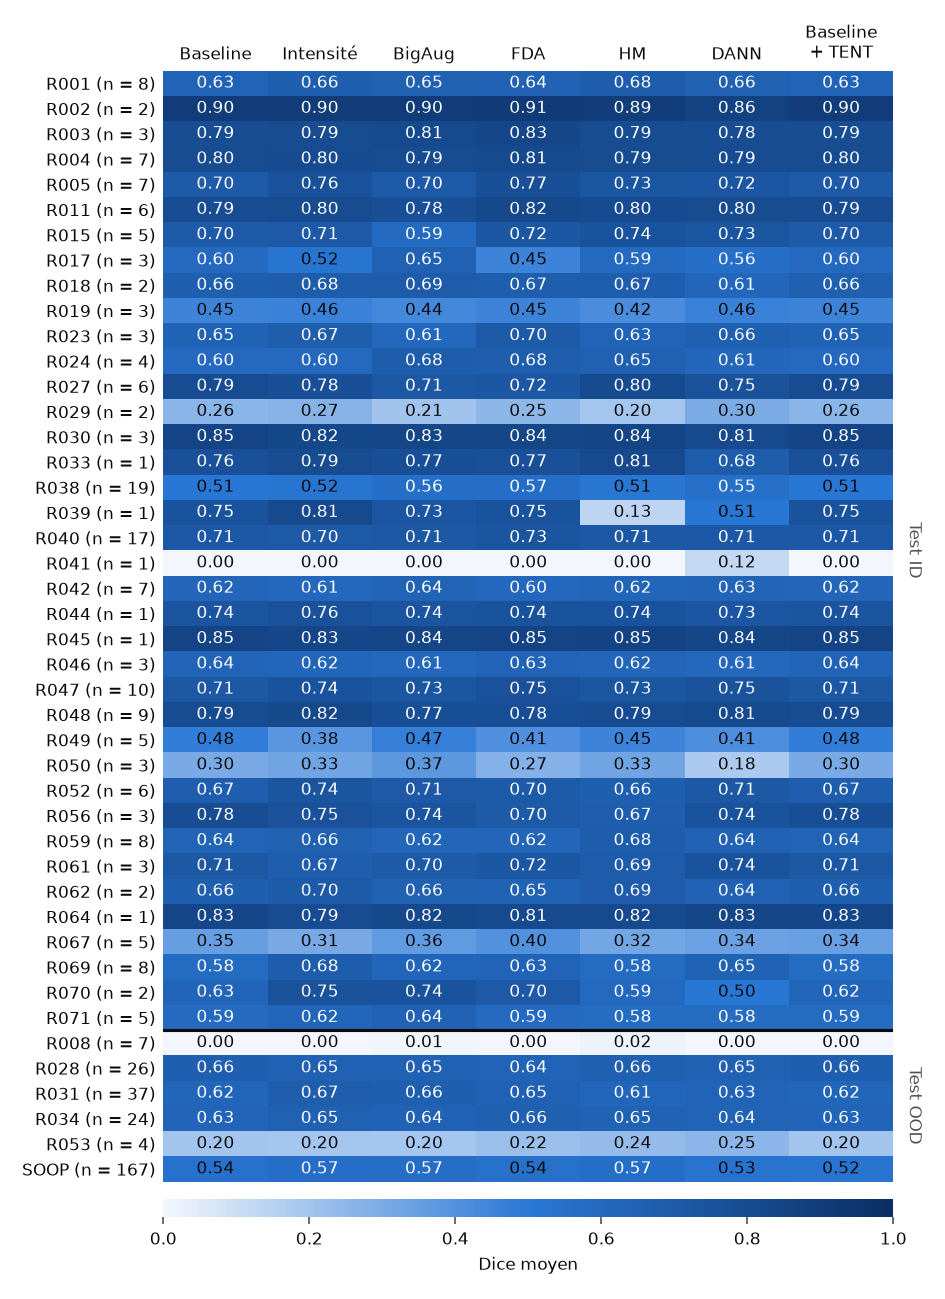
\includegraphics[width=\linewidth]{figures/rq3/rq3_dice_par_centre.png}
  \caption{Dice moyen par centre de test (ID et OOD) et par technique. HM : histogram matching.}
  \label{fig:rq3-dice-centre}
\end{figure}

\subsection{Taille des lésions}

La taille est le facteur le plus net.
Sur les 265 sujets OOD, la corrélation de Spearman entre le volume de la lésion et le Dice (modèle intensité) vaut $\rho = 0{,}53$ ($p < 10^{-4}$).
Le tableau~\ref{tab:rq3-taille} et la figure~\ref{fig:rq3-dice-taille} montrent que toutes les techniques suivent le même profil.
L'intensité gagne surtout entre 1 et 50~ml (0,50 et 0,67 contre 0,46 et 0,64 pour la baseline). BigAug gagne surtout au-dessus de 10~ml (0,68 et 0,77 contre 0,64 et 0,74).

\begin{table}[htbp]
  \centering
  \caption{Dice moyen par volume de lésion sur le test OOD (Dice ID entre parenthèses). L'adaptation continue porte sur un sous-ensemble des sujets.}
  \label{tab:rq3-taille}
  \small
  \begin{tabular}{lcccc}
    \toprule
    Technique & $< 1$~ml & 1--10~ml & 10--50~ml & $\geq 50$~ml \\
    \midrule
    Sujets OOD (ID) & 41 (34) & 86 (65) & 80 (48) & 58 (38) \\
    \midrule
    Baseline & 0,31 (0,48) & 0,46 (0,58) & 0,64 (0,71) & 0,74 (0,83) \\
    Intensité & 0,33 (0,46) & 0,50 (0,59) & 0,67 (0,74) & 0,74 (0,83) \\
    BigAug & 0,32 (0,43) & 0,48 (0,59) & 0,68 (0,75) & 0,77 (0,83) \\
    FDA & 0,30 (0,44) & 0,46 (0,61) & 0,66 (0,74) & 0,75 (0,84) \\
    Histogram matching & 0,33 (0,49) & 0,49 (0,58) & 0,66 (0,71) & 0,74 (0,83) \\
    DANN & 0,29 (0,46) & 0,45 (0,58) & 0,63 (0,73) & 0,75 (0,83) \\
    Baseline + TENT & 0,32 (0,48) & 0,46 (0,58) & 0,62 (0,71) & 0,71 (0,82) \\
    Continue (contrôlée) & 0,35 & 0,48 & 0,60 & 0,81 \\
    \bottomrule
  \end{tabular}
\end{table}

\begin{figure}[htbp]
  \centering
  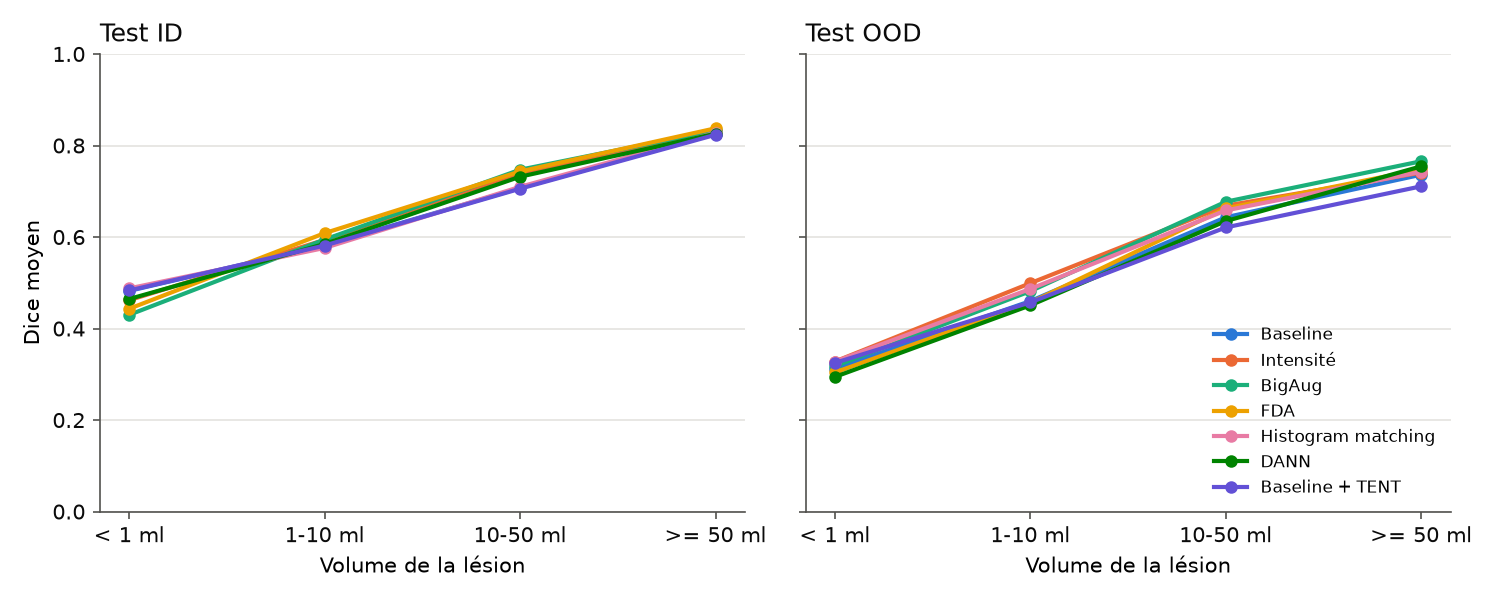
\includegraphics[width=\linewidth]{figures/rq3/rq3_dice_par_taille.png}
  \caption{Dice moyen par classe de volume de lésion, sur les tests ID (à gauche) et OOD (à droite).}
  \label{fig:rq3-dice-taille}
\end{figure}

La figure~\ref{fig:rq3-echecs-taille} reprend le test OOD en y ajoutant l'adaptation continue contrôlée.

\begin{figure}[htbp]
  \centering
  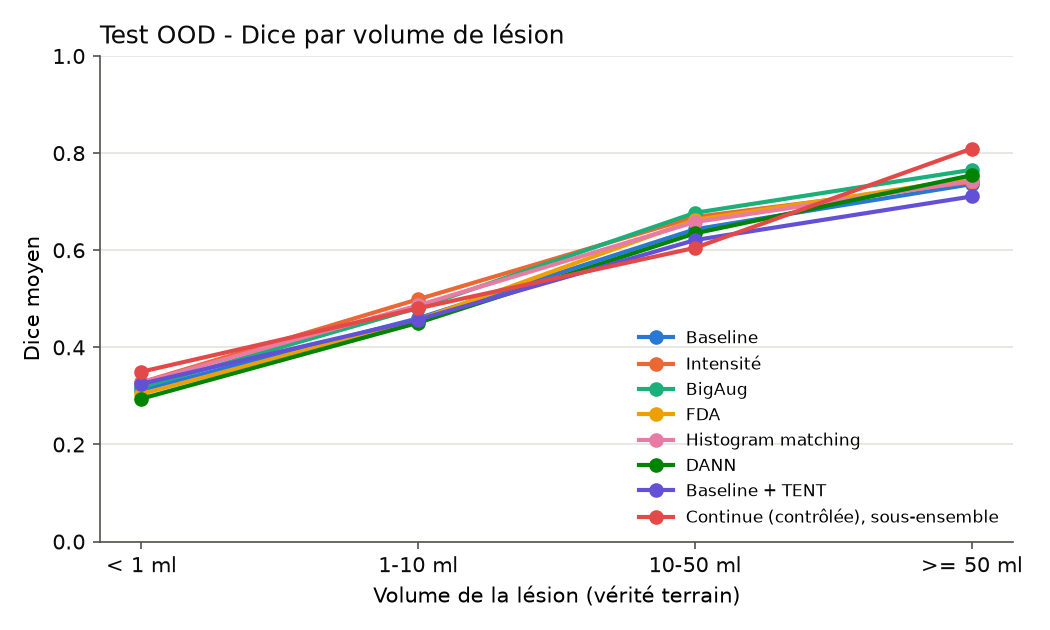
\includegraphics[width=0.8\linewidth]{figures/rq3/rq3_echecs_dice_par_taille.png}
  \caption{Dice moyen par volume de lésion sur le test OOD, avec l'adaptation continue contrôlée (sous-ensemble préquentiel).}
  \label{fig:rq3-echecs-taille}
\end{figure}

\subsection{Centre R008}

Toutes les techniques obtiennent un Dice nul ou presque sur R008. Le Dice moyen de BigAug est de 0,006 sur le centre ; un seul sujet est non nul, à 0,04 (tableau~\ref{tab:rq3-bigaug-intensite} ; moyenne arrondie à 0,01 dans le tableau~\ref{tab:rq3-centres}). Celui d'histogram matching est de 0,019, avec un seul sujet non nul, à 0,13 (tableau~\ref{tab:rq3-hm-intensite}). Le détail par sujet est dans \nolinkurl{zoom_R008_R053.csv}.
\begin{itemize}
  \item Six sujets sur sept sont imagés au premier jour après l'AVC. Leurs lésions font de 0,1 à 4,1~ml.
  \item Les lésions sont peu visibles en T1 : contraste médian de $-0{,}17$, contre $-0{,}50$ à $-0{,}98$ dans les autres centres OOD.
  \item Les intensités sont atypiques : 1,1 à 1,7~\% des voxels du cerveau dépassent $z = 3$, contre 0,003~\% en médiane chez les autres sujets OOD (\nolinkurl{contraste_lesions.csv}).
  \item Le modèle prédit de 0,4 à 33,6~ml répartis en nombreuses composantes, pour une différence du nombre de lésions de 9 à 67.
  \item À l'examen des coupes, vaisseaux, sinus et dure-mère apparaissent hyperintenses.
\end{itemize}
% Les coupes de R008 (figures/rq3/rq3_echecs_coupes_R008.png) ne sont pas incluses :
% ce sont des images ATLAS, non versionnées ; elles se régénèrent avec adaptation/analyse_echecs.py.

\emph{Hypothèse.} La séquence T1 de R008 aurait été acquise après injection de gadolinium, en phase aiguë.
La lésion n'y aurait pas encore le contraste T1 des lésions chroniques, majoritaires à l'entraînement.
Le décalage serait alors à la fois d'acquisition et de stade clinique.
Cette hypothèse reste à vérifier sur le protocole d'acquisition de R008 et sur l'écart entre la date de l'IRM et celle de l'annotation.

\subsection{Centre R053}

Le Dice moyen de R053 est de 0,20 sur quatre sujets ; un cinquième sujet a un masque vide et est exclu du Dice.
Deux lésions minuscules (0,13 et 0,015~ml) ont un Dice de 0. Les deux autres (1,5 et 2,6~ml) obtiennent 0,27 et 0,52.
Les intensités sont dans la norme (99\textsuperscript{e} centile du z-score proche de 1,8) et le contraste vaut $-0{,}50$.
L'échec s'explique par la taille des lésions, pas par un décalage d'intensité. Avec quatre sujets, la moyenne du centre est très instable.

\subsection{Distance de domaine}

La distance de Wasserstein entre histogrammes d'intensité (\nolinkurl{analysis/center_distance.py}, référence = tous les autres centres) ne prédit pas le Dice dans nos runs (\nolinkurl{spearman.csv}).
\begin{itemize}
  \item Sur les six centres OOD, $\rho$ va de $-0{,}43$ à $-0{,}03$ selon la technique ($p$ de 0,40 à 0,96). Avec la MMD, $\rho$ va de $-0{,}37$ à $-0{,}09$.
  \item Sur les 44 centres de test (ID et OOD), $\rho$ va de 0,03 à 0,12 ($p \geq 0{,}44$).
\end{itemize}
La figure~\ref{fig:rq3-distance} en donne deux contre-exemples. R053 est l'un des centres les plus proches (0,020) et l'un des pires. R031 est éloigné (0,164) et parmi les meilleurs.
Six centres offrent une puissance très faible : nous ne concluons pas à l'absence de lien, seulement qu'il n'apparaît pas ici.

\begin{figure}[htbp]
  \centering
  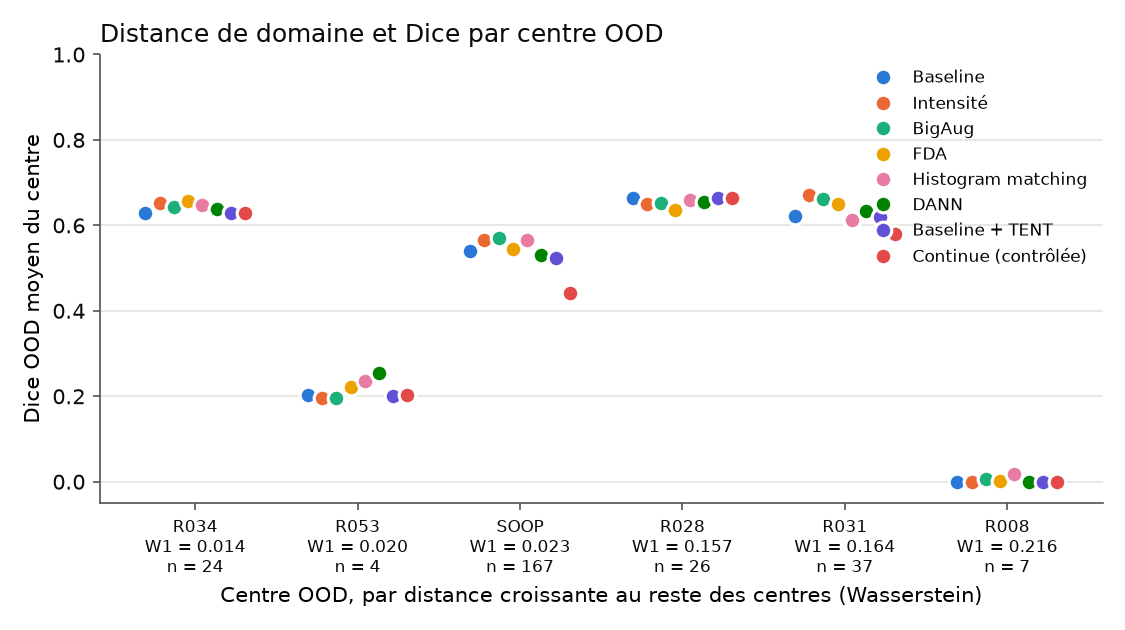
\includegraphics[width=0.8\linewidth]{figures/rq3/rq3_echecs_distance_dice.png}
  \caption{Dice OOD moyen par centre, les centres étant rangés par distance croissante au reste des centres.}
  \label{fig:rq3-distance}
\end{figure}

Au niveau des sujets, le contraste de la lésion n'est que faiblement lié au Dice ($\rho = -0{,}19$, $p = 0{,}001$). La figure~\ref{fig:rq3-contraste} montre ce nuage et place les sujets de R008 et R053.

\begin{figure}[htbp]
  \centering
  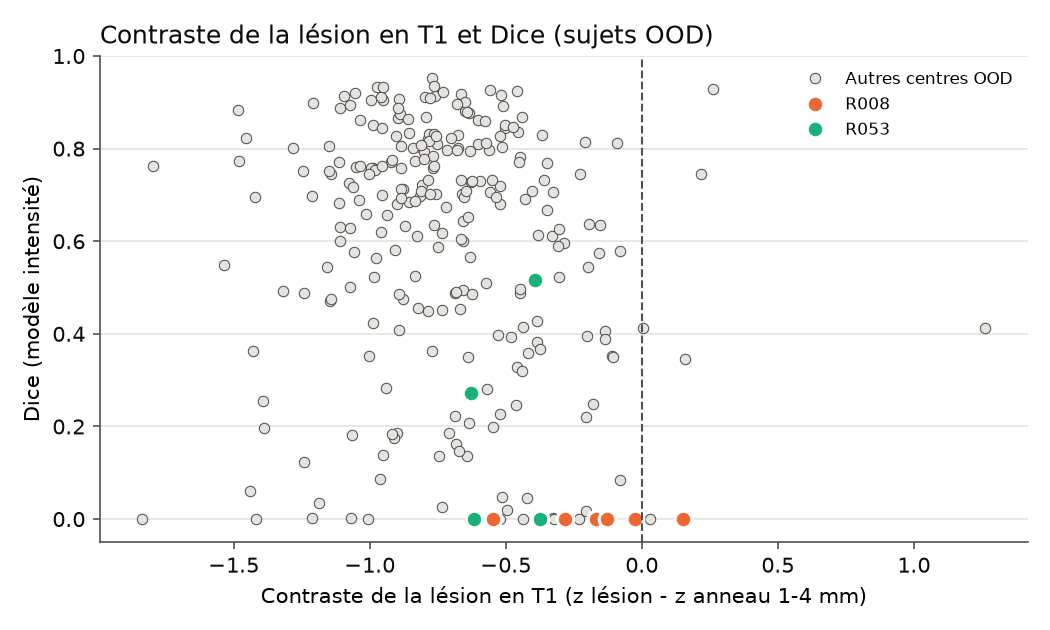
\includegraphics[width=0.8\linewidth]{figures/rq3/rq3_echecs_contraste_dice.png}
  \caption{Contraste T1 de la lésion et Dice (modèle intensité) pour les sujets OOD ; R008 et R053 sont mis en évidence.}
  \label{fig:rq3-contraste}
\end{figure}

\section{Adaptation continue contrôlée}
\label{sec:rq3-continue}

\paragraph{Protocole.}
L'expérience est réalisée par le script \nolinkurl{adaptation/continual.py}.
Ses sorties se trouvent dans le dossier \nolinkurl{adaptation/outputs/rq3/adaptation_continue/}.
Le modèle baseline reçoit les six centres OOD l'un après l'autre, par lots de quatre sujets : 28 lots, 108 sujets, au plus 24 par centre. Il n'est jamais réinitialisé.
L'évaluation est préquentielle : chaque lot est d'abord noté (Dice), puis utilisé pour l'adaptation, sans étiquettes.
Quatre stratégies sont comparées sur les mêmes lots :
\begin{itemize}
  \item \texttt{fige} : le modèle reste inchangé ;
  \item \texttt{auto\_apprentissage} : pseudo-étiquettes, tous les poids sont mis à jour ;
  \item \texttt{tent} : TENT appliqué en continu ;
  \item \texttt{controlee} : TENT dans un modèle candidat, promu seulement si trois conditions sont réunies. (1) La distance du lot dépasse un seuil calibré sur la source (0,077). (2) L'entropie baisse sur des patches neufs. (3) Le Dice sur un jeu de garde étiqueté de la source ne baisse pas de plus de 0,01. Cette stratégie rejoue aussi des exemples des centres déjà vus et des patches de la source.
\end{itemize}
L'oubli est mesuré après chaque centre, par le Dice sur 16 sujets fixes du test ID et sur les premiers sujets des centres OOD déjà vus.

\paragraph{Résultats.}
Le tableau~\ref{tab:rq3-continue} résume les quatre stratégies (\nolinkurl{resume.json}, \nolinkurl{oubli.csv}).

\begin{table}[htbp]
  \centering
  \caption{Adaptation continue sur les six centres OOD : Dice préquentiel et oubli.}
  \label{tab:rq3-continue}
  \small
  \begin{tabular}{lcccc}
    \toprule
    Stratégie & \makecell{Dice\\préquentiel} & \makecell{Dice ID\\(début $\rightarrow$ fin)} & Oubli ID & \makecell{Oubli OOD\\moyen} \\
    \midrule
    Figé & 0,528 & 0,635 $\rightarrow$ 0,635 & 0,000 & 0,000 \\
    Auto-apprentissage & 0,486 & 0,635 $\rightarrow$ 0,583 & 0,052 & 0,033 \\
    TENT continu & 0,526 & 0,635 $\rightarrow$ 0,632 & 0,002 & 0,000 \\
    Contrôlée & 0,527 & 0,635 $\rightarrow$ 0,634 & 0,001 & 0,000 \\
    \bottomrule
  \end{tabular}
\end{table}

Les décisions lot par lot sont dans \nolinkurl{decisions.csv}.
\begin{itemize}
  \item \textbf{Détection.} Un décalage est détecté sur 15 lots sur 28 : tous ceux de R008, R028 et R031, et un lot sur six de SOOP. Il n'est jamais détecté sur R034 ni R053, les centres les plus proches de la source.
  \item \textbf{Promotions.} Douze candidats sont promus : deux pour R008, six pour R028, trois pour R031 et un pour SOOP. Trois candidats de R031 sont refusés parce que leur entropie augmente.
  \item \textbf{Oubli.} La stratégie contrôlée évite l'oubli de l'auto-apprentissage (0,001 contre 0,052 sur le test ID).
  \item \textbf{Gain.} Elle n'améliore pas le Dice par rapport au modèle figé (0,527 contre 0,528).
\end{itemize}

\paragraph{Lecture du résultat.}
L'absence de gain s'explique par la nature des décalages détectés.
R028 et R031 sont déjà bien segmentés par le modèle figé (0,66 et 0,58 en préquentiel).
Sur R008, le problème tient au contraste des lésions (section~\ref{sec:rq3-echecs}), qu'une adaptation des normalisations ne peut pas créer.
Les Dice préquentiels portent sur 108 des 268 sujets OOD ; ils ne se comparent pas directement au tableau~\ref{tab:rq3-resultats}.

\section{Limites}
\label{sec:rq3-limites}

\begin{itemize}
  \item \textbf{Un seul pli et une seule graine.} Les IC traduisent la variabilité des sujets, pas celle de l'entraînement.
  \item \textbf{Reprise de DANN.} La run a été coupée à l'itération 35\,889 et reprise jusqu'à 40\,000. La reprise restaure les poids, l'optimiseur, le taux d'apprentissage, $\lambda$, la position de l'échantillonneur et les états aléatoires des processus de chargement. Le contrôle automatique a validé la première ligne reprise (itération 35\,900, taux $1{,}29 \times 10^{-4}$, $\lambda = 0{,}9771$). Seuls les masques de Dropout du classifieur de centre ne sont pas restaurés. Le meilleur modèle, à l'itération 24\,000, précède de toute façon la coupure.
  \item \textbf{Environnement de DANN.} DANN a été entraînée sur Colab avec torch 2.14.1+cu130 jusqu'à l'itération 35\,889, puis sur Kaggle avec torch 2.11.0+cu130, comme les autres runs. Les deux plateformes utilisent un GPU T4 et CUDA 13.0. Le meilleur modèle (itération 24\,000) vient de la partie Colab. La différence de version de torch peut changer les calculs numériques ; son effet n'a pas été mesuré.
  \item \textbf{Poids de DANN.} Avec un poids de 1, la première run DANN a divergé (perte totale de 10\,508 à l'itération 100 et de 33 millions à l'itération 400). Le poids de 0,1 et la LayerNorm ont été choisis pour la stabilité, sans recherche d'hyperparamètres. Un autre poids pourrait donner un autre résultat.
  \item \textbf{Validation sur des centres non vus.} Ses lésions sont plus petites que celles du test. Elle sert à choisir le checkpoint, mais son Dice (environ 0,43) n'estime pas la performance ID.
  \item \textbf{Diagnostic fp16.} La première baseline, entraînée en fp16, a produit des NaN : des patches entiers donnaient des logits NaN dès l'itération 160 à 180 environ, alors que le fp32 restait stable sur les mêmes lots. Toutes les runs ont été refaites en fp32, environ deux fois plus lentement. La couche qui déborde n'a pas été localisée.
  \item \textbf{Bug de reprise corrigé.} Dans la version du code utilisée pour les runs, la ligne de progression écrasait la file des états aléatoires sauvegardés pour la reprise. Le défaut ne concerne que les reprises, donc uniquement DANN. Il a été corrigé et couvert par un test. Le checkpoint de DANN a été réparé avant la reprise en ne gardant que les quatre derniers états, qui étaient les bons ; les poids n'ont pas changé.
  \item \textbf{Référence de la distance de domaine.} Pour chaque centre, la référence de \nolinkurl{center_distance} regroupe tous les autres centres, OOD compris, et pas seulement les centres d'entraînement du pli~0. La distance mesure donc l'écart au reste du jeu de données, pas exactement l'écart à ce que le modèle a vu.
  \item \textbf{Version du code d'histogram matching.} Cette run a utilisé une version ultérieure du code (\texttt{dbf2f28} au lieu de \texttt{7449c49}), qui ne diffère que par la correction du bug de reprise. Sans DANN ni reprise, les deux versions donnent des poids identiques (vérifié par un court entraînement sur CPU, pour la baseline et l'intensité).
  \item \textbf{Quota GPU.} Avec 30~h par semaine sur Kaggle, aucun autre pli n'a été entraîné, et l'histogram matching a été lancé après les autres techniques.
  \item \textbf{Portée de TENT et de l'adaptation continue.} Les deux ne sont évalués que sur la baseline.
\end{itemize}

\section{Conclusion}
\label{sec:rq3-conclusion}

Sur le pli~0, seule l'augmentation d'intensité améliore le Dice OOD de façon significative après correction : $+0{,}024$ [0,008 ; 0,041], $p$ Holm $= 0{,}0068$ (tableau~\ref{tab:rq3-resultats}).
BigAug atteint le même Dice OOD (0,577), mais son gain n'est pas significatif après correction ($p$ Holm $= 0{,}14$), et la comparaison directe ne sépare pas les deux techniques ($+0{,}001$ [$-0{,}010$ ; 0,012], tableau~\ref{tab:rq3-bigaug-intensite}).
Histogram matching n'est pas significatif non plus ($+0{,}017$, $p$ Holm $= 0{,}49$) ; il reste en dessous de l'intensité en Dice OOD ($-0{,}007$ [$-0{,}023$ ; 0,009]), avec un écart net sur R031 (tableau~\ref{tab:rq3-hm-intensite}).
Aucune technique ne supprime l'écart ID $-$ OOD, qui reste compris entre 0,075 et 0,104.
FDA, DANN et TENT n'améliorent pas le test OOD ; TENT le dégrade légèrement.
L'adaptation continue contrôlée évite l'oubli sans améliorer le Dice (tableau~\ref{tab:rq3-continue}).
L'analyse des échecs montre que les cas les plus difficiles tiennent aux lésions elles-mêmes, petites ou peu contrastées en T1, plutôt qu'à la distance d'intensité entre centres.
Le livrable C8 (\nolinkurl{adaptation/inference.py}) segmente un T1 et renvoie le masque et le volume de la lésion.
Le modèle retenu pour la démonstration est celui de l'intensité.
À Dice égal avec BigAug, ce choix repose d'abord sur son gain significatif après correction, ensuite sur un entraînement plus court (5,0~h contre 8,1~h).
Son F1 des lésions est supérieur à celui de BigAug (0,450 contre 0,420) mais inférieur à celui de la baseline (0,477) : ce n'est qu'un argument relatif face à BigAug.
Histogram matching a le plus faible écart absolu de volume (9,1~ml contre 10,0~ml pour l'intensité) et un F1 des lésions supérieur à celui de la baseline (0,486 contre 0,477).
Il n'a pas été retenu, car son gain en Dice n'est pas significatif et il exigerait d'harmoniser aussi chaque volume à l'inférence, avec l'histogramme de référence de R059.
Ces constats orientent la suite vers la prédiction des cas à risque, en particulier les lésions de moins de 1~ml et les AVC en phase aiguë.
.
% Paquets attendus dans le préambule : babel (french), graphicx, booktabs, makecell, hyperref, float.
% Réglages à mettre dans le préambule du rapport final :
%   \addto\captionsfrench{\def\tablename{Tableau}}   % « Tableau » au lieu de « Table »
%   \hypersetup{hidelinks}                             % liens sans cadre rouge
% Les chemins des figures sont relatifs à la racine du dépôt.
% Citations : docs/rapport/references_rq3.bib, à ajouter à la commande \bibliography du rapport.

\chapter{Généralisation inter-centres (RQ3) et adaptation continue contrôlée}
\label{chap:rq3}

\section{Introduction}
\label{sec:rq3-introduction}

Ce chapitre étudie la robustesse d'un modèle de segmentation des lésions d'AVC face à des centres d'acquisition jamais vus.
La question de recherche RQ3 est la suivante : « Quelles techniques de data augmentation et/ou d'adaptation de domaine réduisent le plus efficacement l'écart de performance entre centres ? »
Nous mesurons cet écart entre des centres vus à l'entraînement (ID) et des centres non vus (OOD).
Nous décrivons d'abord le protocole et les techniques évaluées, puis les résultats et l'analyse des échecs.
Nous présentons ensuite une adaptation continue contrôlée, avant de discuter les limites de l'étude.

\section{Protocole expérimental}
\label{sec:rq3-protocole}

\paragraph{Données.}
Nous utilisons les images T1 d'ATLAS v2.0~\cite{liew2022atlas}, déjà débarrassées du crâne, après le prétraitement S4 de l'équipe : orientation RAS, rééchantillonnage à 1~mm, recadrage sur le cerveau et z-score dans le cerveau (\nolinkurl{preprocessing/week4.py}).
Le découpage est fixé dans \nolinkurl{splits.json}. Le centre R032 est exclu.

\paragraph{Découpage par centre.}
Six centres sont réservés au test OOD : R008, R028, R031, R034, R053 et SOOP.
Ils ont été choisis sur la taille des centres et la distance entre histogrammes d'intensité, sans consulter le Dice (champ \texttt{selection} de \nolinkurl{splits.json}).
Les autres centres sont répartis en cinq plis. Seul le pli~0 a été entraîné. Le tableau~\ref{tab:rq3-donnees} donne les effectifs.

\begin{table}[htbp]
  \centering
  \caption{Effectifs du pli~0.}
  \label{tab:rq3-donnees}
  \begin{tabular}{lrl}
    \toprule
    Ensemble & Sujets & Centres \\
    \midrule
    Entraînement & 733 & 39 \\
    Validation & 183 & 9 centres absents de l'entraînement \\
    Test ID & 185 & centres d'entraînement, sujets non vus \\
    Test OOD & 268 (265 à lésion non vide) & 6 \\
    \bottomrule
  \end{tabular}
\end{table}

Le découpage de \nolinkurl{splits.json} compte 184 sujets de validation.
L'un d'eux, le sujet r065s019 du centre R065, n'a pas de volume prétraité.
Le prétraitement S4 l'a rejeté, car une partie de sa lésion sort du recadrage calculé sur l'image.
Le chargeur l'écarte, et la validation porte donc sur 183 sujets, comme l'indiquent les journaux d'entraînement.
Un de ces 183 sujets a un masque vide : le Dice de validation est calculé sur 182 sujets.

\paragraph{Modèle et entraînement.}
Le réseau est un U-Net~3D de MONAI~\cite{cardoso2022monai} : canaux de 32 à 320, quatre sous-échantillonnages et deux unités résiduelles par niveau.
La normalisation d'instance est affine, ce qu'exige TENT.
L'entraînement utilise des patches de $96^3$ voxels, par lots de quatre patches (deux volumes $\times$ deux patches), dont la moitié est centrée sur la lésion.
Un miroir gauche-droite aléatoire est appliqué à toutes les runs.
La perte combine Dice et entropie croisée.
L'optimiseur AdamW part d'un taux d'apprentissage de $10^{-3}$, avec une décroissance polynomiale (puissance 0,9) et une décroissance des poids de $10^{-5}$.
La norme des gradients est écrêtée à 12.
Toutes les techniques reçoivent le même budget : 40\,000 itérations, graine 2026, calcul en fp32 sur un GPU T4.
Les runs ont été exécutées sur Kaggle (torch 2.11.0+cu130), sauf DANN.
DANN a été entraînée sur Google Colab (GPU T4, torch 2.14.1+cu130) jusqu'à l'itération 35\,889, puis reprise sur Kaggle jusqu'à 40\,000 (section~\ref{sec:rq3-limites}).

\paragraph{Sélection du modèle.}
Le modèle est validé toutes les 2\,000 itérations sur les 183 sujets de validation, en volume entier, par fenêtre glissante de $96^3$ (recouvrement 0,25).
Le checkpoint retenu est celui du meilleur Dice de validation. Il est évalué une seule fois sur les tests ID et OOD.

\paragraph{Métriques.}
Nous rapportons le Dice, la distance de Hausdorff à 95~\% (HD95), l'écart absolu de volume, le F1 des lésions et la différence du nombre de lésions.
Ces métriques sont communes à l'équipe (\nolinkurl{baselines/common.py}).
Le Dice n'est calculé que sur les sujets dont la lésion n'est pas vide.

\paragraph{Tests statistiques.}
Les moyennes sont données avec un intervalle de confiance (IC) à 95~\% par bootstrap percentile (10\,000 tirages).
Pour l'écart ID $-$ OOD, les deux groupes sont rééchantillonnés indépendamment.
Chaque technique est comparée à la baseline par un test des rangs signés de Wilcoxon~\cite{wilcoxon1945}, apparié sur les mêmes sujets.
Une correction de Holm~\cite{holm1979} est appliquée sur l'ensemble des techniques comparées.
La correction porte sur six comparaisons : intensité, BigAug, FDA, histogram matching, DANN et TENT.
BigAug et histogram matching sont aussi comparés directement à l'intensité (différence appariée, IC bootstrap, Wilcoxon), hors correction de Holm : ce sont des comparaisons secondaires avec la technique de référence.

\section{Techniques évaluées}
\label{sec:rq3-techniques}

Toutes les techniques partagent le réseau, les plis, les graines et le budget d'itérations. Seule l'étape propre à chaque technique change (\nolinkurl{adaptation/train.py}, \nolinkurl{generalization/configs/}).

\begin{itemize}
  \item \textbf{Augmentation d'intensité.} Gamma ($p = 0{,}3$) et contraste ($p = 0{,}3$), calibrés sur les seuls sujets d'entraînement ; bruit ($p = 0{,}2$), flou ($p = 0{,}2$), champ de biais ($p = 0{,}3$) et basse résolution ($p = 0{,}25$, jusqu'à 3~mm sur un axe).
  \item \textbf{BigAug}~\cite{zhang2020bigaug}. Flou, netteté, bruit, luminosité, gamma (plage calibrée) et transformation affine (échelle de 0,8 à 1,2, rotation de 20\textdegree), chacun avec $p = 0{,}5$. La déformation élastique est désactivée. Les plages sont adoucies par rapport à l'article pour préserver les petites lésions.
  \item \textbf{FDA} (Fourier Domain Adaptation)~\cite{yang2020fda}. L'amplitude basse fréquence est échangée avec celle d'une image d'un centre d'entraînement de référence (R059 pour le pli~0), avec $\beta$ entre 0,015 et 0,03 et $p = 0{,}5$.
  \item \textbf{DANN} (Domain-Adversarial Neural Network)~\cite{ganin2016dann}. Un classifieur des 39 centres d'entraînement est branché sur la sortie du goulot du réseau : moyenne spatiale, LayerNorm sans paramètres, puis perceptron de 64 unités. Une couche d'inversion du gradient le relie à l'encodeur. Le coefficient $\lambda$ est nul pendant les 2\,000 premières itérations, puis suit la montée proposée par Ganin et al.\ ($\gamma = 5$). La perte du centre a un poids de 0,1.
  \item \textbf{TENT}~\cite{wang2021tent}. Adaptation au test, sans étiquettes, du modèle baseline. Seuls les paramètres affines des normalisations sont modifiés, en minimisant l'entropie des prédictions, centre par centre (Adam, taux de $10^{-4}$, quatre patches par sujet).
  \item \textbf{Histogram matching.} L'histogramme d'intensité du cerveau de chaque volume est ramené vers un histogramme de référence, moyenné sur 20 sujets d'un centre d'entraînement (R059 pour le pli~0). La transformation est déterministe ($p = 1$) et s'applique aussi à la validation et au test. Faute de quota GPU, cette run a été lancée après les autres, avec une version ultérieure du code (section~\ref{sec:rq3-limites}).
\end{itemize}
Fan-Net~\cite{yu2023fannet} n'a pas été implémenté ; FDA en reprend le principe (échange d'amplitude de Fourier) sous une forme plus simple.

\section{Résultats RQ3}
\label{sec:rq3-resultats}

Le tableau~\ref{tab:rq3-resultats} résume les résultats sur 185 sujets ID et 265 sujets OOD (\nolinkurl{adaptation/outputs/rq3/tableau_rq3.md}).

\begin{table}[htbp]
  \centering
  \caption{Dice moyen par technique (pli~0), avec l'IC à 95~\% sous chaque valeur. $\Delta$ OOD : différence appariée à la baseline sur le test OOD ; $p$ : test de Wilcoxon, puis $p$ corrigé par Holm.}
  \label{tab:rq3-resultats}
  \small
  \setlength{\tabcolsep}{4pt}
  \begin{tabular}{lccccc}
    \toprule
    Technique & Dice ID & Dice OOD & \makecell{Écart\\ID $-$ OOD} & $\Delta$ OOD & $p$ OOD \\
    \midrule
    Baseline & \makecell{0,646\\{\footnotesize [0,611 ; 0,680]}} & \makecell{0,553\\{\footnotesize [0,517 ; 0,589]}} & \makecell{0,093\\{\footnotesize [0,044 ; 0,142]}} & -- & -- \\[2pt]
    Intensité & \makecell{0,656\\{\footnotesize [0,621 ; 0,690]}} & \makecell{0,577\\{\footnotesize [0,543 ; 0,611]}} & \makecell{0,080\\{\footnotesize [0,031 ; 0,126]}} & \makecell{+0,024\\{\footnotesize [0,008 ; 0,041]}} & \makecell{0,0014\\{\footnotesize (Holm 0,0068)}} \\[2pt]
    BigAug & \makecell{0,653\\{\footnotesize [0,619 ; 0,686]}} & \makecell{0,577\\{\footnotesize [0,543 ; 0,611]}} & \makecell{0,075\\{\footnotesize [0,028 ; 0,122]}} & \makecell{+0,025\\{\footnotesize [0,010 ; 0,040]}} & \makecell{0,035\\{\footnotesize (Holm 0,14)}} \\[2pt]
    FDA & \makecell{0,660\\{\footnotesize [0,626 ; 0,693]}} & \makecell{0,559\\{\footnotesize [0,524 ; 0,593]}} & \makecell{0,101\\{\footnotesize [0,053 ; 0,148]}} & \makecell{+0,006\\{\footnotesize [$-$0,007 ; 0,020]}} & \makecell{0,32\\{\footnotesize (Holm 0,49)}} \\[2pt]
    \makecell[l]{Histogram\\matching} & \makecell{0,646\\{\footnotesize [0,611 ; 0,681]}} & \makecell{0,570\\{\footnotesize [0,536 ; 0,604]}} & \makecell{0,077\\{\footnotesize [0,027 ; 0,125]}} & \makecell{+0,017\\{\footnotesize [0,001 ; 0,034]}} & \makecell{0,24\\{\footnotesize (Holm 0,49)}} \\[2pt]
    DANN & \makecell{0,650\\{\footnotesize [0,616 ; 0,684]}} & \makecell{0,549\\{\footnotesize [0,513 ; 0,584]}} & \makecell{0,102\\{\footnotesize [0,053 ; 0,150]}} & \makecell{$-$0,004\\{\footnotesize [$-$0,018 ; 0,009]}} & \makecell{0,13\\{\footnotesize (Holm 0,39)}} \\[2pt]
    \makecell[l]{Baseline\\+ TENT} & \makecell{0,645\\{\footnotesize [0,610 ; 0,679]}} & \makecell{0,542\\{\footnotesize [0,506 ; 0,578]}} & \makecell{0,104\\{\footnotesize [0,054 ; 0,153]}} & \makecell{$-$0,011\\{\footnotesize [$-$0,016 ; $-$0,006]}} & \makecell{$< 10^{-4}$\\{\footnotesize (Holm $< 10^{-4}$)}} \\[2pt]
    \bottomrule
  \end{tabular}
\end{table}

La figure~\ref{fig:rq3-dice-id-ood} montre les Dice ID et OOD de chaque technique avec leurs IC.
L'écart entre ID et OOD demeure pour toutes les techniques : il va de 0,075 à 0,104, et aucun IC ne contient 0.

\begin{figure}[htbp]
  \centering
  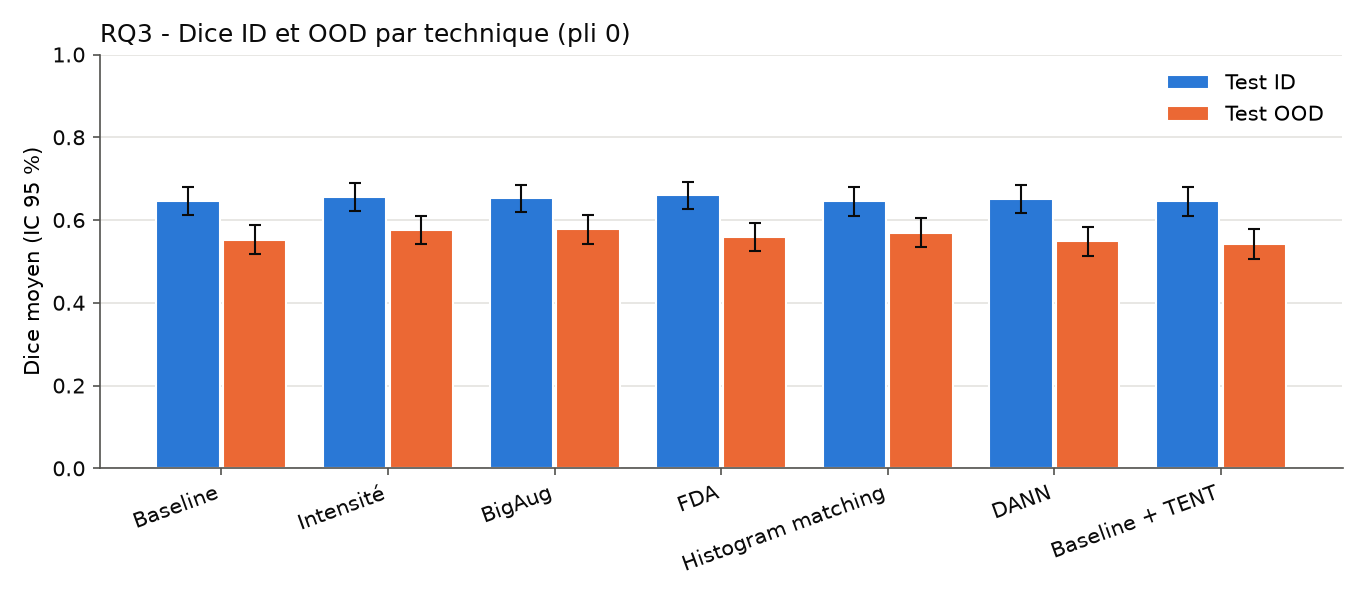
\includegraphics[width=0.8\linewidth]{figures/rq3/rq3_dice_id_ood.png}
  \caption{Dice moyen sur les tests ID et OOD par technique, avec IC à 95~\% (pli~0).}
  \label{fig:rq3-dice-id-ood}
\end{figure}

La figure~\ref{fig:rq3-delta-ood} montre la distribution des différences appariées à la baseline sur le test OOD.
\begin{itemize}
  \item L'augmentation d'intensité est la seule technique qui améliore le Dice OOD de façon significative après correction : $+0{,}024$ [0,008 ; 0,041], $p = 0{,}0014$, $p$ Holm $= 0{,}0068$. Le gain est réparti : 155 sujets sur 252 différences non nulles sont en sa faveur, pour une médiane de $+0{,}006$.
  \item BigAug obtient le même gain moyen ($+0{,}025$ [0,010 ; 0,040]), mais son Wilcoxon ($p = 0{,}035$) n'est plus significatif après correction ($p$ Holm $= 0{,}14$). La différence médiane avec la baseline est quasi nulle ($+0{,}001$ ; 135 sujets en sa faveur sur 250 différences non nulles), et la moyenne est tirée par quelques grands écarts, jusqu'à $+0{,}67$. C'est ce qui explique que le Wilcoxon, fondé sur les rangs, ne passe pas la correction de Holm. Son écart ID $-$ OOD est le plus faible (0,075), mais son IC chevauche celui de la baseline.
  \item FDA a le meilleur Dice ID (0,660), mais son gain sur la baseline n'est significatif après correction ni en ID (Wilcoxon $p = 0{,}012$, $p$ Holm $= 0{,}061$ ; $\Delta$ ID $= +0{,}014$ [$-$0,001 ; 0,029]), ni en OOD ($p = 0{,}32$).
  Avant correction, le Wilcoxon en ID est significatif alors que l'IC bootstrap de $\Delta$ ID contient 0, car les deux ne testent pas la même chose.
  Le Wilcoxon porte sur les rangs des différences appariées : 109 sujets sur 179 différences non nulles sont en faveur de FDA, pour une médiane de $+0{,}005$.
  L'IC porte sur la moyenne, que quelques grandes différences dans les deux sens (jusqu'à $-0{,}32$) rendent plus variable.
  \item Histogram matching améliore le Dice OOD en moyenne ($+0{,}017$ [0,001 ; 0,034]), mais pas de façon significative ($p = 0{,}24$, $p$ Holm $= 0{,}49$). L'IC bootstrap de $\Delta$ OOD exclut tout juste 0 alors que le Wilcoxon n'est pas significatif, pour la même raison que FDA en ID : l'IC porte sur la moyenne, tirée par quelques grands écarts (jusqu'à $+0{,}84$), et le Wilcoxon sur les rangs, avec une médiane nulle (125 sujets en sa faveur, 125 en sa défaveur). Son écart ID $-$ OOD (0,077) est proche de celui de BigAug.
  \item DANN ne se distingue de la baseline ni en ID ($p = 0{,}45$) ni en OOD ($p = 0{,}13$).
  \item TENT abaisse le Dice OOD de 0,011 [0,006 ; 0,016]. L'effet est petit mais systématique ($p < 10^{-4}$). En ID, la baisse est de 0,0007 [0,0002 ; 0,0012] ($p = 1{,}7 \times 10^{-4}$, $p$ Holm $= 1{,}0 \times 10^{-3}$).
\end{itemize}

\begin{figure}[htbp]
  \centering
  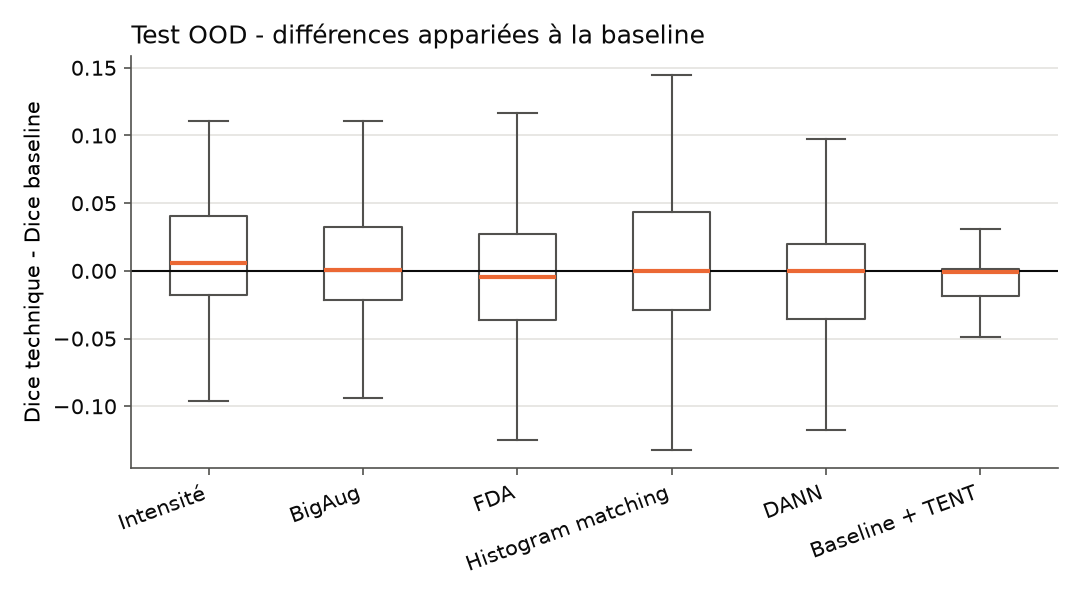
\includegraphics[width=0.8\linewidth]{figures/rq3/rq3_delta_ood.png}
  \caption{Différences appariées de Dice avec la baseline, par sujet, sur le test OOD.}
  \label{fig:rq3-delta-ood}
\end{figure}

\paragraph{BigAug et intensité.}
Le tableau~\ref{tab:rq3-bigaug-intensite} compare directement les deux techniques sur les mêmes sujets (\nolinkurl{adaptation/outputs/rq3/comparaisons.csv}).
Sur le test OOD, la différence moyenne BigAug $-$ intensité vaut $+0{,}001$ [$-0{,}010$ ; 0,012] ($p = 0{,}53$ ; 123 sujets en faveur de BigAug, 128 en faveur de l'intensité).
Sur le test ID, elle vaut $-0{,}003$ [$-0{,}017$ ; 0,011] ($p = 0{,}35$).
Aucun centre OOD ne les sépare : les différences vont de $-0{,}011$ (R034) à $+0{,}006$ (R008), toutes avec $p \geq 0{,}32$.
Les deux techniques sont donc équivalentes en Dice à la précision de cette étude.
Elles diffèrent sur deux points secondaires.
L'entraînement de BigAug dure 8,1~h contre 5,0~h pour l'intensité (\nolinkurl{adaptation/outputs/rq3/entrainement.csv}).
Le F1 des lésions OOD est plus élevé avec l'intensité qu'avec BigAug (0,450 contre 0,420), mais les deux restent sous la baseline (0,477, tableau~\ref{tab:rq3-secondaires}) : ce n'est qu'un avantage relatif face à BigAug.

\begin{table}[htbp]
  \centering
  \caption{Comparaison directe BigAug $-$ intensité par centre OOD (sujets appariés). Source : \texttt{comparaisons\_par\_centre.csv}.}
  \label{tab:rq3-bigaug-intensite}
  \small
  \setlength{\tabcolsep}{4pt}
  \begin{tabular}{lcccccc}
    \toprule
    Centre & n & Dice BigAug & Dice intensité & $\Delta$ moyen & \makecell{Sujets\\BigAug > / < intensité} & $p$ Wilcoxon \\
    \midrule
    R008 & 7 & 0,006 & 0,000 & +0,006 & 1 / 0 & 1 \\
    R028 & 26 & 0,652 & 0,649 & +0,003 & 16 / 10 & 0,50 \\
    R031 & 37 & 0,663 & 0,672 & $-$0,009 & 15 / 22 & 0,32 \\
    R034 & 24 & 0,642 & 0,653 & $-$0,011 & 11 / 12 & 0,76 \\
    R053 & 4 & 0,195 & 0,197 & $-$0,002 & 1 / 1 & 1 \\
    SOOP & 167 & 0,571 & 0,567 & +0,004 & 79 / 83 & 0,60 \\
    \midrule
    Total OOD & 265 & 0,577 & 0,577 & +0,001 & 123 / 128 & 0,53 \\
    \bottomrule
  \end{tabular}
\end{table}

\paragraph{Histogram matching et intensité.}
Le tableau~\ref{tab:rq3-hm-intensite} compare de la même façon histogram matching et intensité.
Sur le test OOD, la différence moyenne histogram matching $-$ intensité vaut $-0{,}007$ [$-0{,}023$ ; 0,009] ($p = 0{,}062$ ; 110 sujets en faveur d'histogram matching, 142 en faveur de l'intensité).
Sur le test ID, elle vaut $-0{,}010$ [$-0{,}025$ ; 0,005] ($p = 0{,}35$).
Le seul écart net par centre concerne R031 : $-0{,}059$ ($p = 0{,}0018$ ; 10 sujets contre 27), qui reste sous 0,05 après une correction de Bonferroni sur les six centres.
Histogram matching a en revanche un F1 des lésions OOD supérieur à celui de la baseline (0,486 contre 0,477) et le plus faible écart absolu de volume de toutes les techniques (9,1~ml, tableau~\ref{tab:rq3-secondaires}).

\begin{table}[htbp]
  \centering
  \caption{Comparaison directe histogram matching $-$ intensité par centre OOD (sujets appariés). HM : histogram matching. Source : \texttt{comparaisons\_par\_centre.csv}.}
  \label{tab:rq3-hm-intensite}
  \small
  \setlength{\tabcolsep}{4pt}
  \begin{tabular}{lcccccc}
    \toprule
    Centre & n & Dice HM & Dice intensité & $\Delta$ moyen & \makecell{Sujets\\HM > / < intensité} & $p$ Wilcoxon \\
    \midrule
    R008 & 7 & 0,019 & 0,000 & +0,019 & 1 / 0 & 1 \\
    R028 & 26 & 0,659 & 0,649 & +0,010 & 16 / 9 & 0,23 \\
    R031 & 37 & 0,614 & 0,672 & $-$0,059 & 10 / 27 & 0,0018 \\
    R034 & 24 & 0,648 & 0,653 & $-$0,005 & 14 / 9 & 0,41 \\
    R053 & 4 & 0,237 & 0,197 & +0,040 & 1 / 1 & 1 \\
    SOOP & 167 & 0,566 & 0,567 & 0,000 & 68 / 96 & 0,11 \\
    \midrule
    Total OOD & 265 & 0,570 & 0,577 & $-$0,007 & 110 / 142 & 0,062 \\
    \bottomrule
  \end{tabular}
\end{table}

\paragraph{Lecture des résultats négatifs.}
Les résultats de DANN et de TENT ne sont pas des défaillances techniques. La run DANN est allée à son terme, avec un contrôle de reprise validé (section~\ref{sec:rq3-limites}). TENT a été appliqué au modèle baseline sur les mêmes sujets. Les deux sont évalués comme les autres techniques.
Pour DANN, l'alignement des caractéristiques entre 39 centres n'apporte rien de mesurable.
Une explication compatible avec nos données est que les échecs OOD dépendent surtout de la taille et du contraste des lésions (section~\ref{sec:rq3-echecs}), deux facteurs que l'alignement des centres ne traite pas.
Pour TENT, la minimisation de l'entropie rend les prédictions plus tranchées sans étiquettes. La baisse touche surtout les lésions de plus de 50~ml (0,71 contre 0,74, tableau~\ref{tab:rq3-taille}).

\paragraph{Métriques secondaires.}
Elles ne suivent pas toujours le Dice (tableau~\ref{tab:rq3-secondaires}).
Le F1 des lésions OOD baisse avec l'intensité (0,450 contre 0,477), BigAug (0,420), FDA et DANN (0,366 et 0,367) ; il augmente avec histogram matching (0,486) et TENT (0,495).
L'écart absolu de volume baisse surtout avec histogram matching (9,1~ml contre 11,1~ml), puis avec l'intensité (10,0~ml) et BigAug (10,9~ml).

\begin{table}[htbp]
  \centering
  \caption{Métriques secondaires moyennes sur le test OOD (\texttt{tableau\_rq3.csv}).}
  \label{tab:rq3-secondaires}
  \begin{tabular}{lccc}
    \toprule
    Technique & F1 des lésions & HD95 (mm) & Écart absolu de volume (ml) \\
    \midrule
    Baseline & 0,477 & 24,9 & 11,1 \\
    Intensité & 0,450 & 25,5 & 10,0 \\
    BigAug & 0,420 & 25,4 & 10,9 \\
    FDA & 0,366 & 26,1 & 13,3 \\
    Histogram matching & 0,486 & 24,9 & 9,1 \\
    DANN & 0,367 & 27,2 & 12,1 \\
    Baseline + TENT & 0,495 & 25,9 & 12,1 \\
    \bottomrule
  \end{tabular}
\end{table}

\paragraph{Validation et test.}
Les meilleurs Dice de validation vont de 0,427 à 0,443 (\nolinkurl{adaptation/outputs/rq3/entrainement.csv}). La validation ne départage donc pas les techniques.
Le Dice de validation (environ 0,43) est plus bas que celui du test ID (0,646) pour deux raisons.
La validation porte sur neuf centres non vus.
Ses lésions sont aussi plus petites : médiane de 1,26~ml et 43~\% sous 1~ml, contre 7,56~ml et 18~\% au test ID (volumes \texttt{lesion\_ml} des fichiers \texttt{qc.json}).

\section{Analyse des échecs}
\label{sec:rq3-echecs}

Les tableaux détaillés de cette section sont produits par le script \nolinkurl{adaptation/analyse_echecs.py}.
Ils se trouvent dans le dossier \nolinkurl{adaptation/outputs/rq3/echecs/}.

\subsection{Dice par centre OOD}

Le tableau~\ref{tab:rq3-centres} et la figure~\ref{fig:rq3-dice-centre} donnent le Dice moyen par centre.
Le contraste T1 est la différence entre le z-score moyen de la lésion et celui d'un anneau de 1 à 4~mm autour d'elle. Une lésion chronique est hypo-intense, et son contraste est négatif.

\begin{table}[htbp]
  \centering
  \caption{Centres OOD, rangés par distance décroissante au reste des centres. Vol. : volume médian des lésions ; J : jours après l'AVC (médiane) ; W1 : distance de Wasserstein ; Base. : baseline ; Int. : intensité ; HM : histogram matching ; TENT : baseline + TENT. Source : \texttt{par\_centre\_ood.csv}.}
  \label{tab:rq3-centres}
  \small
  \setlength{\tabcolsep}{3pt}
  \begin{tabular}{lcccccccccccc}
    \toprule
    & & & & & & \multicolumn{7}{c}{Dice moyen} \\
    \cmidrule(lr){7-13}
    Centre & \makecell{Sujets\\(lésion)} & \makecell{Vol.\\(ml)} & J & W1 & Contraste & Base. & Int. & BigAug & FDA & HM & DANN & TENT \\
    \midrule
    R008 & 7 (7) & 0,95 & 1 & 0,216 & $-$0,17 & 0,00 & 0,00 & 0,01 & 0,00 & 0,02 & 0,00 & 0,00 \\
    R031 & 37 (37) & 6,74 & 138 & 0,164 & $-$0,98 & 0,62 & 0,67 & 0,66 & 0,65 & 0,61 & 0,63 & 0,62 \\
    R028 & 26 (26) & 4,94 & 576 & 0,157 & $-$0,82 & 0,66 & 0,65 & 0,65 & 0,64 & 0,66 & 0,65 & 0,66 \\
    SOOP & 169 (167) & 22,75 & -- & 0,023 & $-$0,69 & 0,54 & 0,57 & 0,57 & 0,54 & 0,57 & 0,53 & 0,52 \\
    R053 & 5 (4) & 0,81 & 25 & 0,020 & $-$0,50 & 0,20 & 0,20 & 0,20 & 0,22 & 0,24 & 0,25 & 0,20 \\
    R034 & 24 (24) & 2,38 & 1\,506 & 0,014 & $-$0,64 & 0,63 & 0,65 & 0,64 & 0,66 & 0,65 & 0,64 & 0,63 \\
    \bottomrule
  \end{tabular}
\end{table}

\begin{figure}[htbp]
  \centering
  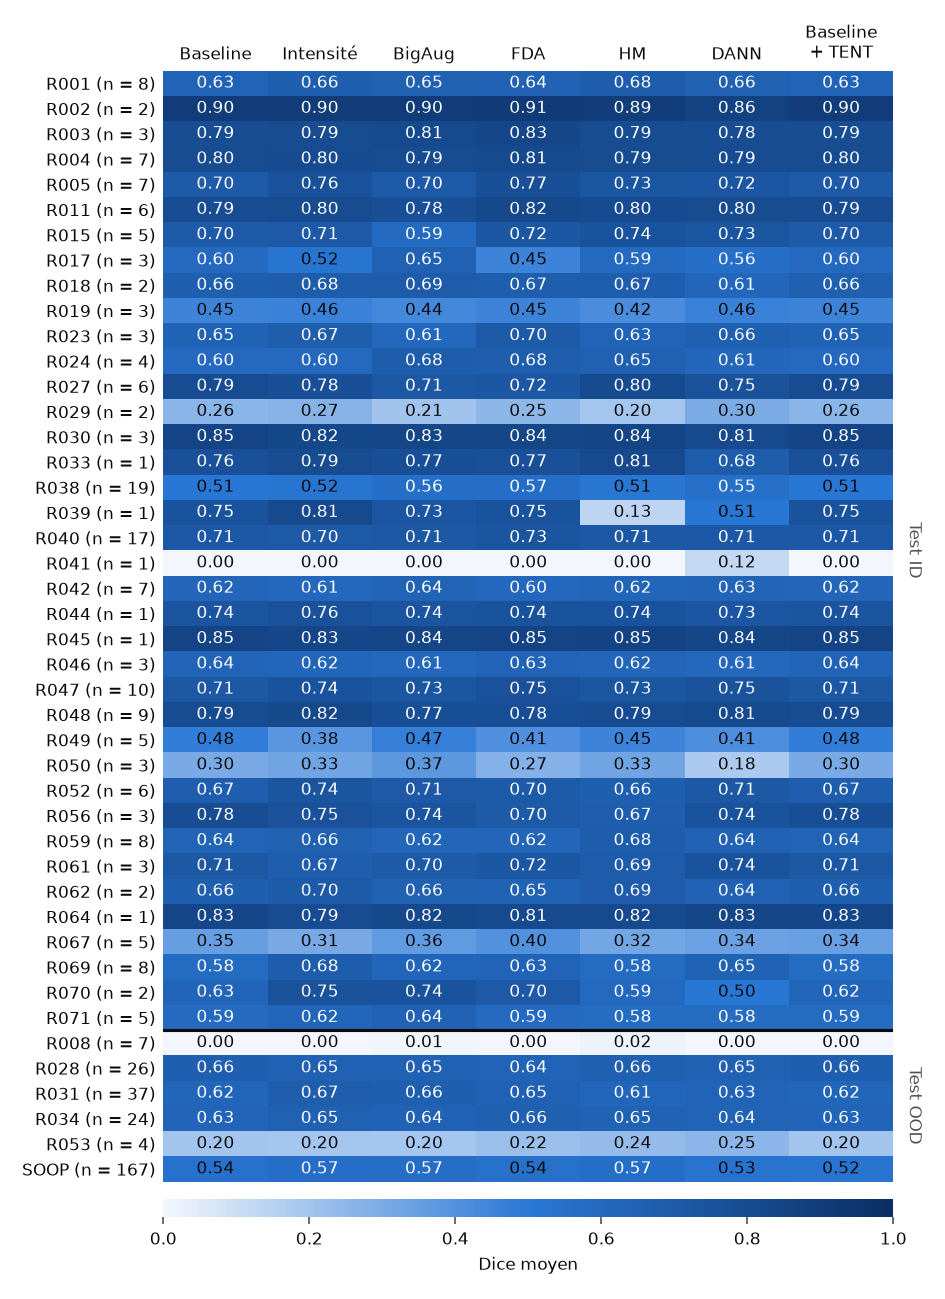
\includegraphics[width=\linewidth]{figures/rq3/rq3_dice_par_centre.png}
  \caption{Dice moyen par centre de test (ID et OOD) et par technique. HM : histogram matching.}
  \label{fig:rq3-dice-centre}
\end{figure}

\subsection{Taille des lésions}

La taille est le facteur le plus net.
Sur les 265 sujets OOD, la corrélation de Spearman entre le volume de la lésion et le Dice (modèle intensité) vaut $\rho = 0{,}53$ ($p < 10^{-4}$).
Le tableau~\ref{tab:rq3-taille} et la figure~\ref{fig:rq3-dice-taille} montrent que toutes les techniques suivent le même profil.
L'intensité gagne surtout entre 1 et 50~ml (0,50 et 0,67 contre 0,46 et 0,64 pour la baseline). BigAug gagne surtout au-dessus de 10~ml (0,68 et 0,77 contre 0,64 et 0,74).

\begin{table}[htbp]
  \centering
  \caption{Dice moyen par volume de lésion sur le test OOD (Dice ID entre parenthèses). L'adaptation continue porte sur un sous-ensemble des sujets.}
  \label{tab:rq3-taille}
  \small
  \begin{tabular}{lcccc}
    \toprule
    Technique & $< 1$~ml & 1--10~ml & 10--50~ml & $\geq 50$~ml \\
    \midrule
    Sujets OOD (ID) & 41 (34) & 86 (65) & 80 (48) & 58 (38) \\
    \midrule
    Baseline & 0,31 (0,48) & 0,46 (0,58) & 0,64 (0,71) & 0,74 (0,83) \\
    Intensité & 0,33 (0,46) & 0,50 (0,59) & 0,67 (0,74) & 0,74 (0,83) \\
    BigAug & 0,32 (0,43) & 0,48 (0,59) & 0,68 (0,75) & 0,77 (0,83) \\
    FDA & 0,30 (0,44) & 0,46 (0,61) & 0,66 (0,74) & 0,75 (0,84) \\
    Histogram matching & 0,33 (0,49) & 0,49 (0,58) & 0,66 (0,71) & 0,74 (0,83) \\
    DANN & 0,29 (0,46) & 0,45 (0,58) & 0,63 (0,73) & 0,75 (0,83) \\
    Baseline + TENT & 0,32 (0,48) & 0,46 (0,58) & 0,62 (0,71) & 0,71 (0,82) \\
    Continue (contrôlée) & 0,35 & 0,48 & 0,60 & 0,81 \\
    \bottomrule
  \end{tabular}
\end{table}

\begin{figure}[htbp]
  \centering
  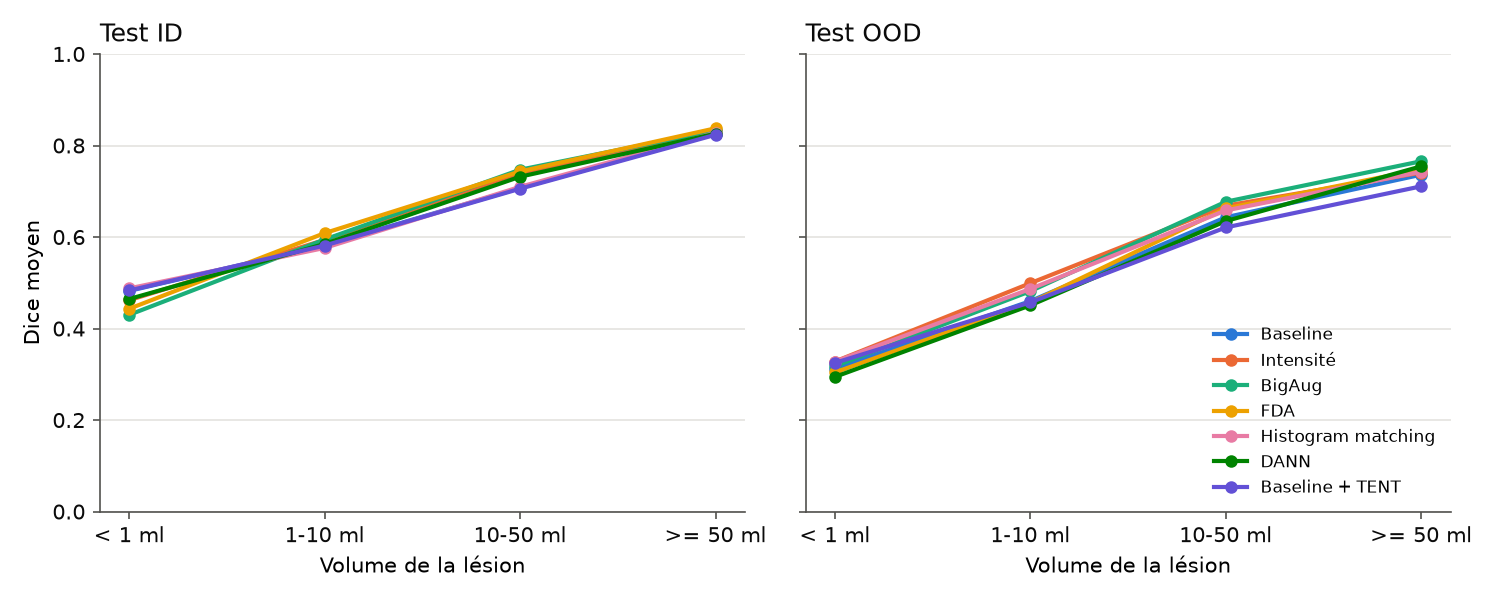
\includegraphics[width=\linewidth]{figures/rq3/rq3_dice_par_taille.png}
  \caption{Dice moyen par classe de volume de lésion, sur les tests ID (à gauche) et OOD (à droite).}
  \label{fig:rq3-dice-taille}
\end{figure}

La figure~\ref{fig:rq3-echecs-taille} reprend le test OOD en y ajoutant l'adaptation continue contrôlée.

\begin{figure}[htbp]
  \centering
  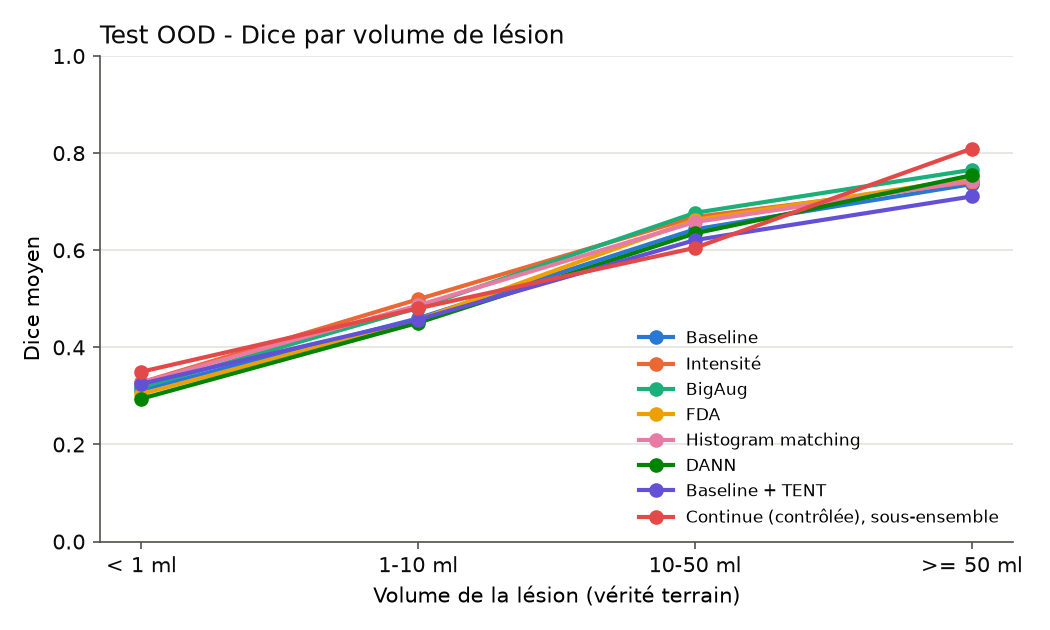
\includegraphics[width=0.8\linewidth]{figures/rq3/rq3_echecs_dice_par_taille.png}
  \caption{Dice moyen par volume de lésion sur le test OOD, avec l'adaptation continue contrôlée (sous-ensemble préquentiel).}
  \label{fig:rq3-echecs-taille}
\end{figure}

\subsection{Centre R008}

Toutes les techniques obtiennent un Dice nul ou presque sur R008. Le Dice moyen de BigAug est de 0,006 sur le centre ; un seul sujet est non nul, à 0,04 (tableau~\ref{tab:rq3-bigaug-intensite} ; moyenne arrondie à 0,01 dans le tableau~\ref{tab:rq3-centres}). Celui d'histogram matching est de 0,019, avec un seul sujet non nul, à 0,13 (tableau~\ref{tab:rq3-hm-intensite}). Le détail par sujet est dans \nolinkurl{zoom_R008_R053.csv}.
\begin{itemize}
  \item Six sujets sur sept sont imagés au premier jour après l'AVC. Leurs lésions font de 0,1 à 4,1~ml.
  \item Les lésions sont peu visibles en T1 : contraste médian de $-0{,}17$, contre $-0{,}50$ à $-0{,}98$ dans les autres centres OOD.
  \item Les intensités sont atypiques : 1,1 à 1,7~\% des voxels du cerveau dépassent $z = 3$, contre 0,003~\% en médiane chez les autres sujets OOD (\nolinkurl{contraste_lesions.csv}).
  \item Le modèle prédit de 0,4 à 33,6~ml répartis en nombreuses composantes, pour une différence du nombre de lésions de 9 à 67.
  \item À l'examen des coupes, vaisseaux, sinus et dure-mère apparaissent hyperintenses.
\end{itemize}
% Les coupes de R008 (figures/rq3/rq3_echecs_coupes_R008.png) ne sont pas incluses :
% ce sont des images ATLAS, non versionnées ; elles se régénèrent avec adaptation/analyse_echecs.py.

\emph{Hypothèse.} La séquence T1 de R008 aurait été acquise après injection de gadolinium, en phase aiguë.
La lésion n'y aurait pas encore le contraste T1 des lésions chroniques, majoritaires à l'entraînement.
Le décalage serait alors à la fois d'acquisition et de stade clinique.
Cette hypothèse reste à vérifier sur le protocole d'acquisition de R008 et sur l'écart entre la date de l'IRM et celle de l'annotation.

\subsection{Centre R053}

Le Dice moyen de R053 est de 0,20 sur quatre sujets ; un cinquième sujet a un masque vide et est exclu du Dice.
Deux lésions minuscules (0,13 et 0,015~ml) ont un Dice de 0. Les deux autres (1,5 et 2,6~ml) obtiennent 0,27 et 0,52.
Les intensités sont dans la norme (99\textsuperscript{e} centile du z-score proche de 1,8) et le contraste vaut $-0{,}50$.
L'échec s'explique par la taille des lésions, pas par un décalage d'intensité. Avec quatre sujets, la moyenne du centre est très instable.

\subsection{Distance de domaine}

La distance de Wasserstein entre histogrammes d'intensité (\nolinkurl{analysis/center_distance.py}, référence = tous les autres centres) ne prédit pas le Dice dans nos runs (\nolinkurl{spearman.csv}).
\begin{itemize}
  \item Sur les six centres OOD, $\rho$ va de $-0{,}43$ à $-0{,}03$ selon la technique ($p$ de 0,40 à 0,96). Avec la MMD, $\rho$ va de $-0{,}37$ à $-0{,}09$.
  \item Sur les 44 centres de test (ID et OOD), $\rho$ va de 0,03 à 0,12 ($p \geq 0{,}44$).
\end{itemize}
La figure~\ref{fig:rq3-distance} en donne deux contre-exemples. R053 est l'un des centres les plus proches (0,020) et l'un des pires. R031 est éloigné (0,164) et parmi les meilleurs.
Six centres offrent une puissance très faible : nous ne concluons pas à l'absence de lien, seulement qu'il n'apparaît pas ici.

\begin{figure}[htbp]
  \centering
  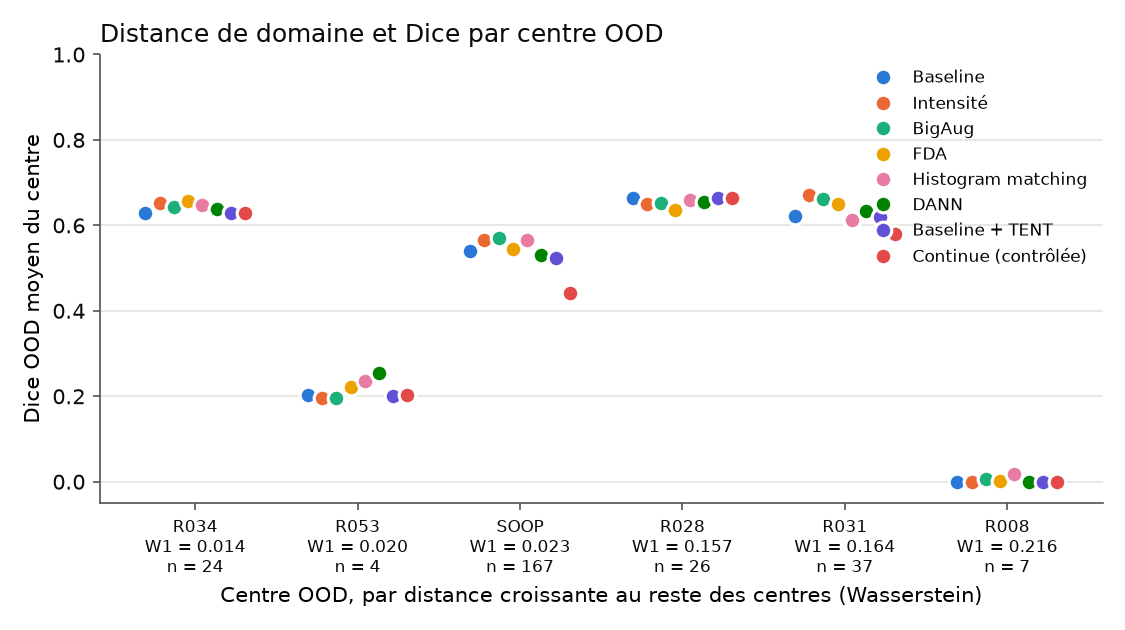
\includegraphics[width=0.8\linewidth]{figures/rq3/rq3_echecs_distance_dice.png}
  \caption{Dice OOD moyen par centre, les centres étant rangés par distance croissante au reste des centres.}
  \label{fig:rq3-distance}
\end{figure}

Au niveau des sujets, le contraste de la lésion n'est que faiblement lié au Dice ($\rho = -0{,}19$, $p = 0{,}001$). La figure~\ref{fig:rq3-contraste} montre ce nuage et place les sujets de R008 et R053.

\begin{figure}[htbp]
  \centering
  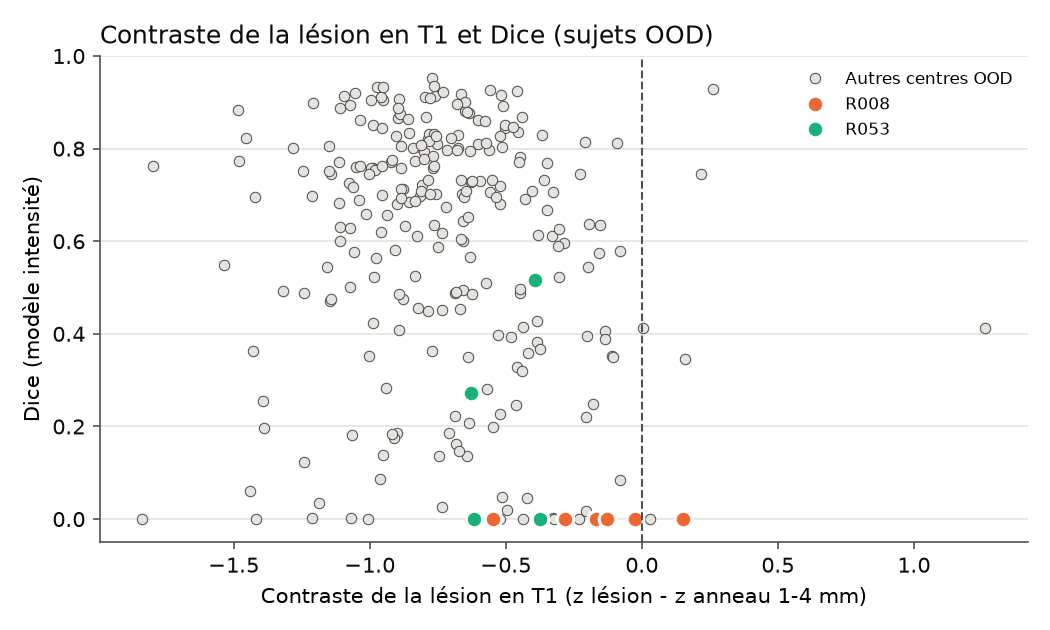
\includegraphics[width=0.8\linewidth]{figures/rq3/rq3_echecs_contraste_dice.png}
  \caption{Contraste T1 de la lésion et Dice (modèle intensité) pour les sujets OOD ; R008 et R053 sont mis en évidence.}
  \label{fig:rq3-contraste}
\end{figure}

\section{Adaptation continue contrôlée}
\label{sec:rq3-continue}

\paragraph{Protocole.}
L'expérience est réalisée par le script \nolinkurl{adaptation/continual.py}.
Ses sorties se trouvent dans le dossier \nolinkurl{adaptation/outputs/rq3/adaptation_continue/}.
Le modèle baseline reçoit les six centres OOD l'un après l'autre, par lots de quatre sujets : 28 lots, 108 sujets, au plus 24 par centre. Il n'est jamais réinitialisé.
L'évaluation est préquentielle : chaque lot est d'abord noté (Dice), puis utilisé pour l'adaptation, sans étiquettes.
Quatre stratégies sont comparées sur les mêmes lots :
\begin{itemize}
  \item \texttt{fige} : le modèle reste inchangé ;
  \item \texttt{auto\_apprentissage} : pseudo-étiquettes, tous les poids sont mis à jour ;
  \item \texttt{tent} : TENT appliqué en continu ;
  \item \texttt{controlee} : TENT dans un modèle candidat, promu seulement si trois conditions sont réunies. (1) La distance du lot dépasse un seuil calibré sur la source (0,077). (2) L'entropie baisse sur des patches neufs. (3) Le Dice sur un jeu de garde étiqueté de la source ne baisse pas de plus de 0,01. Cette stratégie rejoue aussi des exemples des centres déjà vus et des patches de la source.
\end{itemize}
L'oubli est mesuré après chaque centre, par le Dice sur 16 sujets fixes du test ID et sur les premiers sujets des centres OOD déjà vus.

\paragraph{Résultats.}
Le tableau~\ref{tab:rq3-continue} résume les quatre stratégies (\nolinkurl{resume.json}, \nolinkurl{oubli.csv}).

\begin{table}[htbp]
  \centering
  \caption{Adaptation continue sur les six centres OOD : Dice préquentiel et oubli.}
  \label{tab:rq3-continue}
  \small
  \begin{tabular}{lcccc}
    \toprule
    Stratégie & \makecell{Dice\\préquentiel} & \makecell{Dice ID\\(début $\rightarrow$ fin)} & Oubli ID & \makecell{Oubli OOD\\moyen} \\
    \midrule
    Figé & 0,528 & 0,635 $\rightarrow$ 0,635 & 0,000 & 0,000 \\
    Auto-apprentissage & 0,486 & 0,635 $\rightarrow$ 0,583 & 0,052 & 0,033 \\
    TENT continu & 0,526 & 0,635 $\rightarrow$ 0,632 & 0,002 & 0,000 \\
    Contrôlée & 0,527 & 0,635 $\rightarrow$ 0,634 & 0,001 & 0,000 \\
    \bottomrule
  \end{tabular}
\end{table}

Les décisions lot par lot sont dans \nolinkurl{decisions.csv}.
\begin{itemize}
  \item \textbf{Détection.} Un décalage est détecté sur 15 lots sur 28 : tous ceux de R008, R028 et R031, et un lot sur six de SOOP. Il n'est jamais détecté sur R034 ni R053, les centres les plus proches de la source.
  \item \textbf{Promotions.} Douze candidats sont promus : deux pour R008, six pour R028, trois pour R031 et un pour SOOP. Trois candidats de R031 sont refusés parce que leur entropie augmente.
  \item \textbf{Oubli.} La stratégie contrôlée évite l'oubli de l'auto-apprentissage (0,001 contre 0,052 sur le test ID).
  \item \textbf{Gain.} Elle n'améliore pas le Dice par rapport au modèle figé (0,527 contre 0,528).
\end{itemize}

\paragraph{Lecture du résultat.}
L'absence de gain s'explique par la nature des décalages détectés.
R028 et R031 sont déjà bien segmentés par le modèle figé (0,66 et 0,58 en préquentiel).
Sur R008, le problème tient au contraste des lésions (section~\ref{sec:rq3-echecs}), qu'une adaptation des normalisations ne peut pas créer.
Les Dice préquentiels portent sur 108 des 268 sujets OOD ; ils ne se comparent pas directement au tableau~\ref{tab:rq3-resultats}.

\section{Limites}
\label{sec:rq3-limites}

\begin{itemize}
  \item \textbf{Un seul pli et une seule graine.} Les IC traduisent la variabilité des sujets, pas celle de l'entraînement.
  \item \textbf{Reprise de DANN.} La run a été coupée à l'itération 35\,889 et reprise jusqu'à 40\,000. La reprise restaure les poids, l'optimiseur, le taux d'apprentissage, $\lambda$, la position de l'échantillonneur et les états aléatoires des processus de chargement. Le contrôle automatique a validé la première ligne reprise (itération 35\,900, taux $1{,}29 \times 10^{-4}$, $\lambda = 0{,}9771$). Seuls les masques de Dropout du classifieur de centre ne sont pas restaurés. Le meilleur modèle, à l'itération 24\,000, précède de toute façon la coupure.
  \item \textbf{Environnement de DANN.} DANN a été entraînée sur Colab avec torch 2.14.1+cu130 jusqu'à l'itération 35\,889, puis sur Kaggle avec torch 2.11.0+cu130, comme les autres runs. Les deux plateformes utilisent un GPU T4 et CUDA 13.0. Le meilleur modèle (itération 24\,000) vient de la partie Colab. La différence de version de torch peut changer les calculs numériques ; son effet n'a pas été mesuré.
  \item \textbf{Poids de DANN.} Avec un poids de 1, la première run DANN a divergé (perte totale de 10\,508 à l'itération 100 et de 33 millions à l'itération 400). Le poids de 0,1 et la LayerNorm ont été choisis pour la stabilité, sans recherche d'hyperparamètres. Un autre poids pourrait donner un autre résultat.
  \item \textbf{Validation sur des centres non vus.} Ses lésions sont plus petites que celles du test. Elle sert à choisir le checkpoint, mais son Dice (environ 0,43) n'estime pas la performance ID.
  \item \textbf{Diagnostic fp16.} La première baseline, entraînée en fp16, a produit des NaN : des patches entiers donnaient des logits NaN dès l'itération 160 à 180 environ, alors que le fp32 restait stable sur les mêmes lots. Toutes les runs ont été refaites en fp32, environ deux fois plus lentement. La couche qui déborde n'a pas été localisée.
  \item \textbf{Bug de reprise corrigé.} Dans la version du code utilisée pour les runs, la ligne de progression écrasait la file des états aléatoires sauvegardés pour la reprise. Le défaut ne concerne que les reprises, donc uniquement DANN. Il a été corrigé et couvert par un test. Le checkpoint de DANN a été réparé avant la reprise en ne gardant que les quatre derniers états, qui étaient les bons ; les poids n'ont pas changé.
  \item \textbf{Référence de la distance de domaine.} Pour chaque centre, la référence de \nolinkurl{center_distance} regroupe tous les autres centres, OOD compris, et pas seulement les centres d'entraînement du pli~0. La distance mesure donc l'écart au reste du jeu de données, pas exactement l'écart à ce que le modèle a vu.
  \item \textbf{Version du code d'histogram matching.} Cette run a utilisé une version ultérieure du code (\texttt{dbf2f28} au lieu de \texttt{7449c49}), qui ne diffère que par la correction du bug de reprise. Sans DANN ni reprise, les deux versions donnent des poids identiques (vérifié par un court entraînement sur CPU, pour la baseline et l'intensité).
  \item \textbf{Quota GPU.} Avec 30~h par semaine sur Kaggle, aucun autre pli n'a été entraîné, et l'histogram matching a été lancé après les autres techniques.
  \item \textbf{Portée de TENT et de l'adaptation continue.} Les deux ne sont évalués que sur la baseline.
\end{itemize}

\section{Conclusion}
\label{sec:rq3-conclusion}

Sur le pli~0, seule l'augmentation d'intensité améliore le Dice OOD de façon significative après correction : $+0{,}024$ [0,008 ; 0,041], $p$ Holm $= 0{,}0068$ (tableau~\ref{tab:rq3-resultats}).
BigAug atteint le même Dice OOD (0,577), mais son gain n'est pas significatif après correction ($p$ Holm $= 0{,}14$), et la comparaison directe ne sépare pas les deux techniques ($+0{,}001$ [$-0{,}010$ ; 0,012], tableau~\ref{tab:rq3-bigaug-intensite}).
Histogram matching n'est pas significatif non plus ($+0{,}017$, $p$ Holm $= 0{,}49$) ; il reste en dessous de l'intensité en Dice OOD ($-0{,}007$ [$-0{,}023$ ; 0,009]), avec un écart net sur R031 (tableau~\ref{tab:rq3-hm-intensite}).
Aucune technique ne supprime l'écart ID $-$ OOD, qui reste compris entre 0,075 et 0,104.
FDA, DANN et TENT n'améliorent pas le test OOD ; TENT le dégrade légèrement.
L'adaptation continue contrôlée évite l'oubli sans améliorer le Dice (tableau~\ref{tab:rq3-continue}).
L'analyse des échecs montre que les cas les plus difficiles tiennent aux lésions elles-mêmes, petites ou peu contrastées en T1, plutôt qu'à la distance d'intensité entre centres.
Le livrable C8 (\nolinkurl{adaptation/inference.py}) segmente un T1 et renvoie le masque et le volume de la lésion.
Le modèle retenu pour la démonstration est celui de l'intensité.
À Dice égal avec BigAug, ce choix repose d'abord sur son gain significatif après correction, ensuite sur un entraînement plus court (5,0~h contre 8,1~h).
Son F1 des lésions est supérieur à celui de BigAug (0,450 contre 0,420) mais inférieur à celui de la baseline (0,477) : ce n'est qu'un argument relatif face à BigAug.
Histogram matching a le plus faible écart absolu de volume (9,1~ml contre 10,0~ml pour l'intensité) et un F1 des lésions supérieur à celui de la baseline (0,486 contre 0,477).
Il n'a pas été retenu, car son gain en Dice n'est pas significatif et il exigerait d'harmoniser aussi chaque volume à l'inférence, avec l'histogramme de référence de R059.
Ces constats orientent la suite vers la prédiction des cas à risque, en particulier les lésions de moins de 1~ml et les AVC en phase aiguë.
.
% Paquets attendus dans le préambule : babel (french), graphicx, booktabs, makecell, hyperref, float.
% Réglages à mettre dans le préambule du rapport final :
%   \addto\captionsfrench{\def\tablename{Tableau}}   % « Tableau » au lieu de « Table »
%   \hypersetup{hidelinks}                             % liens sans cadre rouge
% Les chemins des figures sont relatifs à la racine du dépôt.
% Citations : docs/rapport/references_rq3.bib, à ajouter à la commande \bibliography du rapport.

\chapter{Généralisation inter-centres (RQ3) et adaptation continue contrôlée}
\label{chap:rq3}

\section{Introduction}
\label{sec:rq3-introduction}

Ce chapitre étudie la robustesse d'un modèle de segmentation des lésions d'AVC face à des centres d'acquisition jamais vus.
La question de recherche RQ3 est la suivante : « Quelles techniques de data augmentation et/ou d'adaptation de domaine réduisent le plus efficacement l'écart de performance entre centres ? »
Nous mesurons cet écart entre des centres vus à l'entraînement (ID) et des centres non vus (OOD).
Nous décrivons d'abord le protocole et les techniques évaluées, puis les résultats et l'analyse des échecs.
Nous présentons ensuite une adaptation continue contrôlée, avant de discuter les limites de l'étude.

\section{Protocole expérimental}
\label{sec:rq3-protocole}

\paragraph{Données.}
Nous utilisons les images T1 d'ATLAS v2.0~\cite{liew2022atlas}, déjà débarrassées du crâne, après le prétraitement S4 de l'équipe : orientation RAS, rééchantillonnage à 1~mm, recadrage sur le cerveau et z-score dans le cerveau (\nolinkurl{preprocessing/week4.py}).
Le découpage est fixé dans \nolinkurl{splits.json}. Le centre R032 est exclu.

\paragraph{Découpage par centre.}
Six centres sont réservés au test OOD : R008, R028, R031, R034, R053 et SOOP.
Ils ont été choisis sur la taille des centres et la distance entre histogrammes d'intensité, sans consulter le Dice (champ \texttt{selection} de \nolinkurl{splits.json}).
Les autres centres sont répartis en cinq plis. Seul le pli~0 a été entraîné. Le tableau~\ref{tab:rq3-donnees} donne les effectifs.

\begin{table}[htbp]
  \centering
  \caption{Effectifs du pli~0.}
  \label{tab:rq3-donnees}
  \begin{tabular}{lrl}
    \toprule
    Ensemble & Sujets & Centres \\
    \midrule
    Entraînement & 733 & 39 \\
    Validation & 183 & 9 centres absents de l'entraînement \\
    Test ID & 185 & centres d'entraînement, sujets non vus \\
    Test OOD & 268 (265 à lésion non vide) & 6 \\
    \bottomrule
  \end{tabular}
\end{table}

Le découpage de \nolinkurl{splits.json} compte 184 sujets de validation.
L'un d'eux, le sujet r065s019 du centre R065, n'a pas de volume prétraité.
Le prétraitement S4 l'a rejeté, car une partie de sa lésion sort du recadrage calculé sur l'image.
Le chargeur l'écarte, et la validation porte donc sur 183 sujets, comme l'indiquent les journaux d'entraînement.
Un de ces 183 sujets a un masque vide : le Dice de validation est calculé sur 182 sujets.

\paragraph{Modèle et entraînement.}
Le réseau est un U-Net~3D de MONAI~\cite{cardoso2022monai} : canaux de 32 à 320, quatre sous-échantillonnages et deux unités résiduelles par niveau.
La normalisation d'instance est affine, ce qu'exige TENT.
L'entraînement utilise des patches de $96^3$ voxels, par lots de quatre patches (deux volumes $\times$ deux patches), dont la moitié est centrée sur la lésion.
Un miroir gauche-droite aléatoire est appliqué à toutes les runs.
La perte combine Dice et entropie croisée.
L'optimiseur AdamW part d'un taux d'apprentissage de $10^{-3}$, avec une décroissance polynomiale (puissance 0,9) et une décroissance des poids de $10^{-5}$.
La norme des gradients est écrêtée à 12.
Toutes les techniques reçoivent le même budget : 40\,000 itérations, graine 2026, calcul en fp32 sur un GPU T4.
Les runs ont été exécutées sur Kaggle (torch 2.11.0+cu130), sauf DANN.
DANN a été entraînée sur Google Colab (GPU T4, torch 2.14.1+cu130) jusqu'à l'itération 35\,889, puis reprise sur Kaggle jusqu'à 40\,000 (section~\ref{sec:rq3-limites}).

\paragraph{Sélection du modèle.}
Le modèle est validé toutes les 2\,000 itérations sur les 183 sujets de validation, en volume entier, par fenêtre glissante de $96^3$ (recouvrement 0,25).
Le checkpoint retenu est celui du meilleur Dice de validation. Il est évalué une seule fois sur les tests ID et OOD.

\paragraph{Métriques.}
Nous rapportons le Dice, la distance de Hausdorff à 95~\% (HD95), l'écart absolu de volume, le F1 des lésions et la différence du nombre de lésions.
Ces métriques sont communes à l'équipe (\nolinkurl{baselines/common.py}).
Le Dice n'est calculé que sur les sujets dont la lésion n'est pas vide.

\paragraph{Tests statistiques.}
Les moyennes sont données avec un intervalle de confiance (IC) à 95~\% par bootstrap percentile (10\,000 tirages).
Pour l'écart ID $-$ OOD, les deux groupes sont rééchantillonnés indépendamment.
Chaque technique est comparée à la baseline par un test des rangs signés de Wilcoxon~\cite{wilcoxon1945}, apparié sur les mêmes sujets.
Une correction de Holm~\cite{holm1979} est appliquée sur l'ensemble des techniques comparées.
La correction porte sur six comparaisons : intensité, BigAug, FDA, histogram matching, DANN et TENT.
BigAug et histogram matching sont aussi comparés directement à l'intensité (différence appariée, IC bootstrap, Wilcoxon), hors correction de Holm : ce sont des comparaisons secondaires avec la technique de référence.

\section{Techniques évaluées}
\label{sec:rq3-techniques}

Toutes les techniques partagent le réseau, les plis, les graines et le budget d'itérations. Seule l'étape propre à chaque technique change (\nolinkurl{adaptation/train.py}, \nolinkurl{generalization/configs/}).

\begin{itemize}
  \item \textbf{Augmentation d'intensité.} Gamma ($p = 0{,}3$) et contraste ($p = 0{,}3$), calibrés sur les seuls sujets d'entraînement ; bruit ($p = 0{,}2$), flou ($p = 0{,}2$), champ de biais ($p = 0{,}3$) et basse résolution ($p = 0{,}25$, jusqu'à 3~mm sur un axe).
  \item \textbf{BigAug}~\cite{zhang2020bigaug}. Flou, netteté, bruit, luminosité, gamma (plage calibrée) et transformation affine (échelle de 0,8 à 1,2, rotation de 20\textdegree), chacun avec $p = 0{,}5$. La déformation élastique est désactivée. Les plages sont adoucies par rapport à l'article pour préserver les petites lésions.
  \item \textbf{FDA} (Fourier Domain Adaptation)~\cite{yang2020fda}. L'amplitude basse fréquence est échangée avec celle d'une image d'un centre d'entraînement de référence (R059 pour le pli~0), avec $\beta$ entre 0,015 et 0,03 et $p = 0{,}5$.
  \item \textbf{DANN} (Domain-Adversarial Neural Network)~\cite{ganin2016dann}. Un classifieur des 39 centres d'entraînement est branché sur la sortie du goulot du réseau : moyenne spatiale, LayerNorm sans paramètres, puis perceptron de 64 unités. Une couche d'inversion du gradient le relie à l'encodeur. Le coefficient $\lambda$ est nul pendant les 2\,000 premières itérations, puis suit la montée proposée par Ganin et al.\ ($\gamma = 5$). La perte du centre a un poids de 0,1.
  \item \textbf{TENT}~\cite{wang2021tent}. Adaptation au test, sans étiquettes, du modèle baseline. Seuls les paramètres affines des normalisations sont modifiés, en minimisant l'entropie des prédictions, centre par centre (Adam, taux de $10^{-4}$, quatre patches par sujet).
  \item \textbf{Histogram matching.} L'histogramme d'intensité du cerveau de chaque volume est ramené vers un histogramme de référence, moyenné sur 20 sujets d'un centre d'entraînement (R059 pour le pli~0). La transformation est déterministe ($p = 1$) et s'applique aussi à la validation et au test. Faute de quota GPU, cette run a été lancée après les autres, avec une version ultérieure du code (section~\ref{sec:rq3-limites}).
\end{itemize}
Fan-Net~\cite{yu2023fannet} n'a pas été implémenté ; FDA en reprend le principe (échange d'amplitude de Fourier) sous une forme plus simple.

\section{Résultats RQ3}
\label{sec:rq3-resultats}

Le tableau~\ref{tab:rq3-resultats} résume les résultats sur 185 sujets ID et 265 sujets OOD (\nolinkurl{adaptation/outputs/rq3/tableau_rq3.md}).

\begin{table}[htbp]
  \centering
  \caption{Dice moyen par technique (pli~0), avec l'IC à 95~\% sous chaque valeur. $\Delta$ OOD : différence appariée à la baseline sur le test OOD ; $p$ : test de Wilcoxon, puis $p$ corrigé par Holm.}
  \label{tab:rq3-resultats}
  \small
  \setlength{\tabcolsep}{4pt}
  \begin{tabular}{lccccc}
    \toprule
    Technique & Dice ID & Dice OOD & \makecell{Écart\\ID $-$ OOD} & $\Delta$ OOD & $p$ OOD \\
    \midrule
    Baseline & \makecell{0,646\\{\footnotesize [0,611 ; 0,680]}} & \makecell{0,553\\{\footnotesize [0,517 ; 0,589]}} & \makecell{0,093\\{\footnotesize [0,044 ; 0,142]}} & -- & -- \\[2pt]
    Intensité & \makecell{0,656\\{\footnotesize [0,621 ; 0,690]}} & \makecell{0,577\\{\footnotesize [0,543 ; 0,611]}} & \makecell{0,080\\{\footnotesize [0,031 ; 0,126]}} & \makecell{+0,024\\{\footnotesize [0,008 ; 0,041]}} & \makecell{0,0014\\{\footnotesize (Holm 0,0068)}} \\[2pt]
    BigAug & \makecell{0,653\\{\footnotesize [0,619 ; 0,686]}} & \makecell{0,577\\{\footnotesize [0,543 ; 0,611]}} & \makecell{0,075\\{\footnotesize [0,028 ; 0,122]}} & \makecell{+0,025\\{\footnotesize [0,010 ; 0,040]}} & \makecell{0,035\\{\footnotesize (Holm 0,14)}} \\[2pt]
    FDA & \makecell{0,660\\{\footnotesize [0,626 ; 0,693]}} & \makecell{0,559\\{\footnotesize [0,524 ; 0,593]}} & \makecell{0,101\\{\footnotesize [0,053 ; 0,148]}} & \makecell{+0,006\\{\footnotesize [$-$0,007 ; 0,020]}} & \makecell{0,32\\{\footnotesize (Holm 0,49)}} \\[2pt]
    \makecell[l]{Histogram\\matching} & \makecell{0,646\\{\footnotesize [0,611 ; 0,681]}} & \makecell{0,570\\{\footnotesize [0,536 ; 0,604]}} & \makecell{0,077\\{\footnotesize [0,027 ; 0,125]}} & \makecell{+0,017\\{\footnotesize [0,001 ; 0,034]}} & \makecell{0,24\\{\footnotesize (Holm 0,49)}} \\[2pt]
    DANN & \makecell{0,650\\{\footnotesize [0,616 ; 0,684]}} & \makecell{0,549\\{\footnotesize [0,513 ; 0,584]}} & \makecell{0,102\\{\footnotesize [0,053 ; 0,150]}} & \makecell{$-$0,004\\{\footnotesize [$-$0,018 ; 0,009]}} & \makecell{0,13\\{\footnotesize (Holm 0,39)}} \\[2pt]
    \makecell[l]{Baseline\\+ TENT} & \makecell{0,645\\{\footnotesize [0,610 ; 0,679]}} & \makecell{0,542\\{\footnotesize [0,506 ; 0,578]}} & \makecell{0,104\\{\footnotesize [0,054 ; 0,153]}} & \makecell{$-$0,011\\{\footnotesize [$-$0,016 ; $-$0,006]}} & \makecell{$< 10^{-4}$\\{\footnotesize (Holm $< 10^{-4}$)}} \\[2pt]
    \bottomrule
  \end{tabular}
\end{table}

La figure~\ref{fig:rq3-dice-id-ood} montre les Dice ID et OOD de chaque technique avec leurs IC.
L'écart entre ID et OOD demeure pour toutes les techniques : il va de 0,075 à 0,104, et aucun IC ne contient 0.

\begin{figure}[htbp]
  \centering
  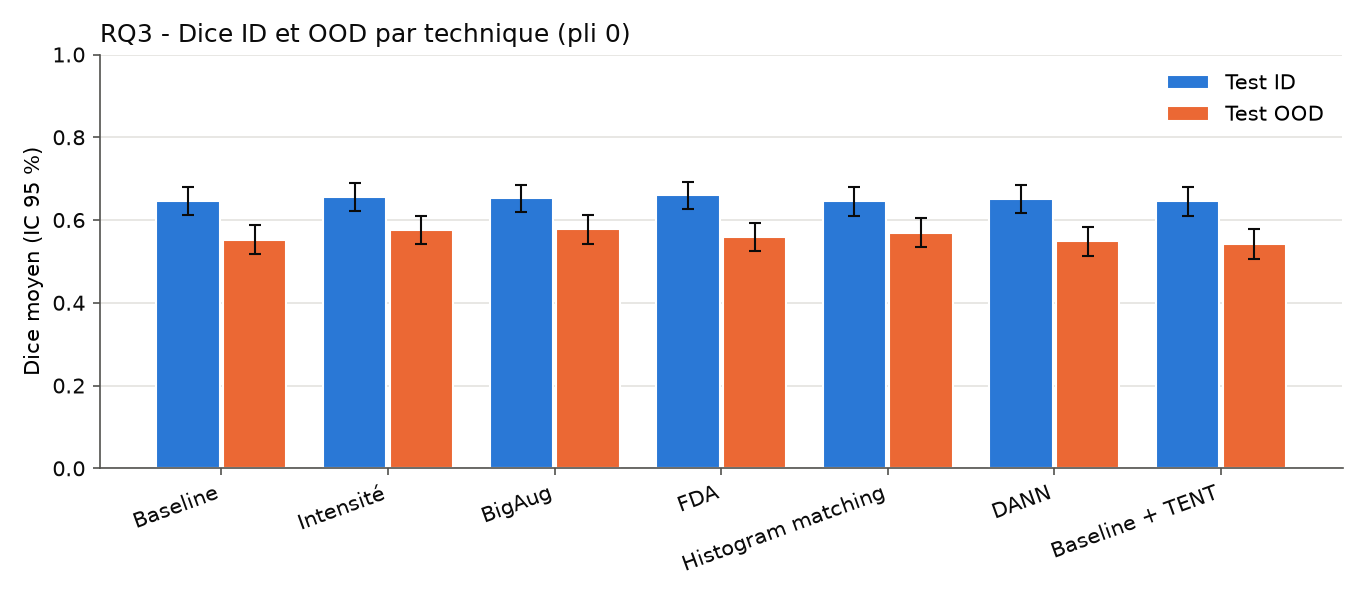
\includegraphics[width=0.8\linewidth]{figures/rq3/rq3_dice_id_ood.png}
  \caption{Dice moyen sur les tests ID et OOD par technique, avec IC à 95~\% (pli~0).}
  \label{fig:rq3-dice-id-ood}
\end{figure}

La figure~\ref{fig:rq3-delta-ood} montre la distribution des différences appariées à la baseline sur le test OOD.
\begin{itemize}
  \item L'augmentation d'intensité est la seule technique qui améliore le Dice OOD de façon significative après correction : $+0{,}024$ [0,008 ; 0,041], $p = 0{,}0014$, $p$ Holm $= 0{,}0068$. Le gain est réparti : 155 sujets sur 252 différences non nulles sont en sa faveur, pour une médiane de $+0{,}006$.
  \item BigAug obtient le même gain moyen ($+0{,}025$ [0,010 ; 0,040]), mais son Wilcoxon ($p = 0{,}035$) n'est plus significatif après correction ($p$ Holm $= 0{,}14$). La différence médiane avec la baseline est quasi nulle ($+0{,}001$ ; 135 sujets en sa faveur sur 250 différences non nulles), et la moyenne est tirée par quelques grands écarts, jusqu'à $+0{,}67$. C'est ce qui explique que le Wilcoxon, fondé sur les rangs, ne passe pas la correction de Holm. Son écart ID $-$ OOD est le plus faible (0,075), mais son IC chevauche celui de la baseline.
  \item FDA a le meilleur Dice ID (0,660), mais son gain sur la baseline n'est significatif après correction ni en ID (Wilcoxon $p = 0{,}012$, $p$ Holm $= 0{,}061$ ; $\Delta$ ID $= +0{,}014$ [$-$0,001 ; 0,029]), ni en OOD ($p = 0{,}32$).
  Avant correction, le Wilcoxon en ID est significatif alors que l'IC bootstrap de $\Delta$ ID contient 0, car les deux ne testent pas la même chose.
  Le Wilcoxon porte sur les rangs des différences appariées : 109 sujets sur 179 différences non nulles sont en faveur de FDA, pour une médiane de $+0{,}005$.
  L'IC porte sur la moyenne, que quelques grandes différences dans les deux sens (jusqu'à $-0{,}32$) rendent plus variable.
  \item Histogram matching améliore le Dice OOD en moyenne ($+0{,}017$ [0,001 ; 0,034]), mais pas de façon significative ($p = 0{,}24$, $p$ Holm $= 0{,}49$). L'IC bootstrap de $\Delta$ OOD exclut tout juste 0 alors que le Wilcoxon n'est pas significatif, pour la même raison que FDA en ID : l'IC porte sur la moyenne, tirée par quelques grands écarts (jusqu'à $+0{,}84$), et le Wilcoxon sur les rangs, avec une médiane nulle (125 sujets en sa faveur, 125 en sa défaveur). Son écart ID $-$ OOD (0,077) est proche de celui de BigAug.
  \item DANN ne se distingue de la baseline ni en ID ($p = 0{,}45$) ni en OOD ($p = 0{,}13$).
  \item TENT abaisse le Dice OOD de 0,011 [0,006 ; 0,016]. L'effet est petit mais systématique ($p < 10^{-4}$). En ID, la baisse est de 0,0007 [0,0002 ; 0,0012] ($p = 1{,}7 \times 10^{-4}$, $p$ Holm $= 1{,}0 \times 10^{-3}$).
\end{itemize}

\begin{figure}[htbp]
  \centering
  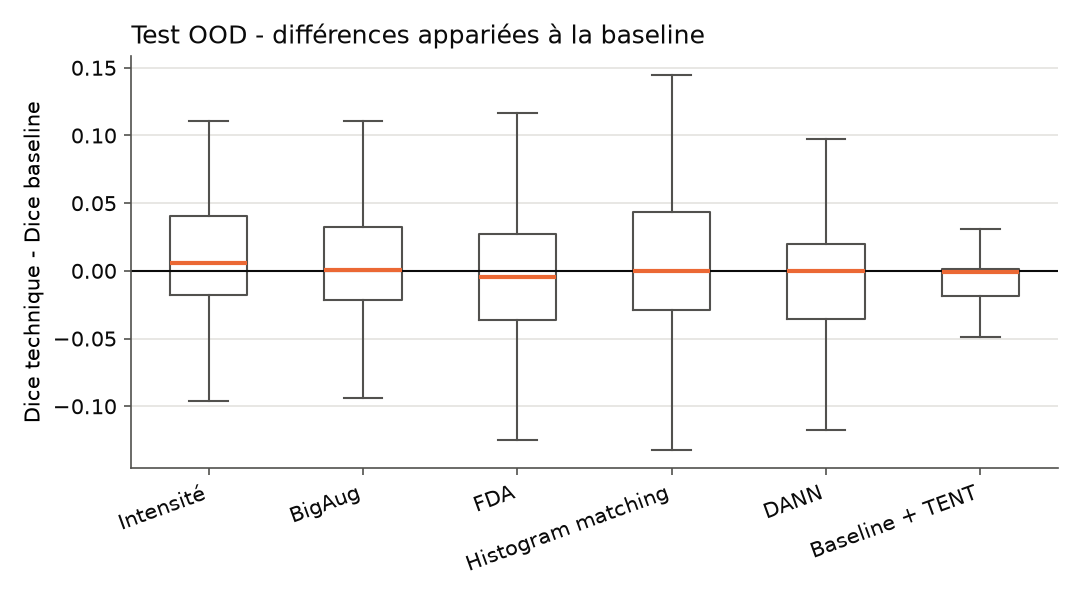
\includegraphics[width=0.8\linewidth]{figures/rq3/rq3_delta_ood.png}
  \caption{Différences appariées de Dice avec la baseline, par sujet, sur le test OOD.}
  \label{fig:rq3-delta-ood}
\end{figure}

\paragraph{BigAug et intensité.}
Le tableau~\ref{tab:rq3-bigaug-intensite} compare directement les deux techniques sur les mêmes sujets (\nolinkurl{adaptation/outputs/rq3/comparaisons.csv}).
Sur le test OOD, la différence moyenne BigAug $-$ intensité vaut $+0{,}001$ [$-0{,}010$ ; 0,012] ($p = 0{,}53$ ; 123 sujets en faveur de BigAug, 128 en faveur de l'intensité).
Sur le test ID, elle vaut $-0{,}003$ [$-0{,}017$ ; 0,011] ($p = 0{,}35$).
Aucun centre OOD ne les sépare : les différences vont de $-0{,}011$ (R034) à $+0{,}006$ (R008), toutes avec $p \geq 0{,}32$.
Les deux techniques sont donc équivalentes en Dice à la précision de cette étude.
Elles diffèrent sur deux points secondaires.
L'entraînement de BigAug dure 8,1~h contre 5,0~h pour l'intensité (\nolinkurl{adaptation/outputs/rq3/entrainement.csv}).
Le F1 des lésions OOD est plus élevé avec l'intensité qu'avec BigAug (0,450 contre 0,420), mais les deux restent sous la baseline (0,477, tableau~\ref{tab:rq3-secondaires}) : ce n'est qu'un avantage relatif face à BigAug.

\begin{table}[htbp]
  \centering
  \caption{Comparaison directe BigAug $-$ intensité par centre OOD (sujets appariés). Source : \texttt{comparaisons\_par\_centre.csv}.}
  \label{tab:rq3-bigaug-intensite}
  \small
  \setlength{\tabcolsep}{4pt}
  \begin{tabular}{lcccccc}
    \toprule
    Centre & n & Dice BigAug & Dice intensité & $\Delta$ moyen & \makecell{Sujets\\BigAug > / < intensité} & $p$ Wilcoxon \\
    \midrule
    R008 & 7 & 0,006 & 0,000 & +0,006 & 1 / 0 & 1 \\
    R028 & 26 & 0,652 & 0,649 & +0,003 & 16 / 10 & 0,50 \\
    R031 & 37 & 0,663 & 0,672 & $-$0,009 & 15 / 22 & 0,32 \\
    R034 & 24 & 0,642 & 0,653 & $-$0,011 & 11 / 12 & 0,76 \\
    R053 & 4 & 0,195 & 0,197 & $-$0,002 & 1 / 1 & 1 \\
    SOOP & 167 & 0,571 & 0,567 & +0,004 & 79 / 83 & 0,60 \\
    \midrule
    Total OOD & 265 & 0,577 & 0,577 & +0,001 & 123 / 128 & 0,53 \\
    \bottomrule
  \end{tabular}
\end{table}

\paragraph{Histogram matching et intensité.}
Le tableau~\ref{tab:rq3-hm-intensite} compare de la même façon histogram matching et intensité.
Sur le test OOD, la différence moyenne histogram matching $-$ intensité vaut $-0{,}007$ [$-0{,}023$ ; 0,009] ($p = 0{,}062$ ; 110 sujets en faveur d'histogram matching, 142 en faveur de l'intensité).
Sur le test ID, elle vaut $-0{,}010$ [$-0{,}025$ ; 0,005] ($p = 0{,}35$).
Le seul écart net par centre concerne R031 : $-0{,}059$ ($p = 0{,}0018$ ; 10 sujets contre 27), qui reste sous 0,05 après une correction de Bonferroni sur les six centres.
Histogram matching a en revanche un F1 des lésions OOD supérieur à celui de la baseline (0,486 contre 0,477) et le plus faible écart absolu de volume de toutes les techniques (9,1~ml, tableau~\ref{tab:rq3-secondaires}).

\begin{table}[htbp]
  \centering
  \caption{Comparaison directe histogram matching $-$ intensité par centre OOD (sujets appariés). HM : histogram matching. Source : \texttt{comparaisons\_par\_centre.csv}.}
  \label{tab:rq3-hm-intensite}
  \small
  \setlength{\tabcolsep}{4pt}
  \begin{tabular}{lcccccc}
    \toprule
    Centre & n & Dice HM & Dice intensité & $\Delta$ moyen & \makecell{Sujets\\HM > / < intensité} & $p$ Wilcoxon \\
    \midrule
    R008 & 7 & 0,019 & 0,000 & +0,019 & 1 / 0 & 1 \\
    R028 & 26 & 0,659 & 0,649 & +0,010 & 16 / 9 & 0,23 \\
    R031 & 37 & 0,614 & 0,672 & $-$0,059 & 10 / 27 & 0,0018 \\
    R034 & 24 & 0,648 & 0,653 & $-$0,005 & 14 / 9 & 0,41 \\
    R053 & 4 & 0,237 & 0,197 & +0,040 & 1 / 1 & 1 \\
    SOOP & 167 & 0,566 & 0,567 & 0,000 & 68 / 96 & 0,11 \\
    \midrule
    Total OOD & 265 & 0,570 & 0,577 & $-$0,007 & 110 / 142 & 0,062 \\
    \bottomrule
  \end{tabular}
\end{table}

\paragraph{Lecture des résultats négatifs.}
Les résultats de DANN et de TENT ne sont pas des défaillances techniques. La run DANN est allée à son terme, avec un contrôle de reprise validé (section~\ref{sec:rq3-limites}). TENT a été appliqué au modèle baseline sur les mêmes sujets. Les deux sont évalués comme les autres techniques.
Pour DANN, l'alignement des caractéristiques entre 39 centres n'apporte rien de mesurable.
Une explication compatible avec nos données est que les échecs OOD dépendent surtout de la taille et du contraste des lésions (section~\ref{sec:rq3-echecs}), deux facteurs que l'alignement des centres ne traite pas.
Pour TENT, la minimisation de l'entropie rend les prédictions plus tranchées sans étiquettes. La baisse touche surtout les lésions de plus de 50~ml (0,71 contre 0,74, tableau~\ref{tab:rq3-taille}).

\paragraph{Métriques secondaires.}
Elles ne suivent pas toujours le Dice (tableau~\ref{tab:rq3-secondaires}).
Le F1 des lésions OOD baisse avec l'intensité (0,450 contre 0,477), BigAug (0,420), FDA et DANN (0,366 et 0,367) ; il augmente avec histogram matching (0,486) et TENT (0,495).
L'écart absolu de volume baisse surtout avec histogram matching (9,1~ml contre 11,1~ml), puis avec l'intensité (10,0~ml) et BigAug (10,9~ml).

\begin{table}[htbp]
  \centering
  \caption{Métriques secondaires moyennes sur le test OOD (\texttt{tableau\_rq3.csv}).}
  \label{tab:rq3-secondaires}
  \begin{tabular}{lccc}
    \toprule
    Technique & F1 des lésions & HD95 (mm) & Écart absolu de volume (ml) \\
    \midrule
    Baseline & 0,477 & 24,9 & 11,1 \\
    Intensité & 0,450 & 25,5 & 10,0 \\
    BigAug & 0,420 & 25,4 & 10,9 \\
    FDA & 0,366 & 26,1 & 13,3 \\
    Histogram matching & 0,486 & 24,9 & 9,1 \\
    DANN & 0,367 & 27,2 & 12,1 \\
    Baseline + TENT & 0,495 & 25,9 & 12,1 \\
    \bottomrule
  \end{tabular}
\end{table}

\paragraph{Validation et test.}
Les meilleurs Dice de validation vont de 0,427 à 0,443 (\nolinkurl{adaptation/outputs/rq3/entrainement.csv}). La validation ne départage donc pas les techniques.
Le Dice de validation (environ 0,43) est plus bas que celui du test ID (0,646) pour deux raisons.
La validation porte sur neuf centres non vus.
Ses lésions sont aussi plus petites : médiane de 1,26~ml et 43~\% sous 1~ml, contre 7,56~ml et 18~\% au test ID (volumes \texttt{lesion\_ml} des fichiers \texttt{qc.json}).

\section{Analyse des échecs}
\label{sec:rq3-echecs}

Les tableaux détaillés de cette section sont produits par le script \nolinkurl{adaptation/analyse_echecs.py}.
Ils se trouvent dans le dossier \nolinkurl{adaptation/outputs/rq3/echecs/}.

\subsection{Dice par centre OOD}

Le tableau~\ref{tab:rq3-centres} et la figure~\ref{fig:rq3-dice-centre} donnent le Dice moyen par centre.
Le contraste T1 est la différence entre le z-score moyen de la lésion et celui d'un anneau de 1 à 4~mm autour d'elle. Une lésion chronique est hypo-intense, et son contraste est négatif.

\begin{table}[htbp]
  \centering
  \caption{Centres OOD, rangés par distance décroissante au reste des centres. Vol. : volume médian des lésions ; J : jours après l'AVC (médiane) ; W1 : distance de Wasserstein ; Base. : baseline ; Int. : intensité ; HM : histogram matching ; TENT : baseline + TENT. Source : \texttt{par\_centre\_ood.csv}.}
  \label{tab:rq3-centres}
  \small
  \setlength{\tabcolsep}{3pt}
  \begin{tabular}{lcccccccccccc}
    \toprule
    & & & & & & \multicolumn{7}{c}{Dice moyen} \\
    \cmidrule(lr){7-13}
    Centre & \makecell{Sujets\\(lésion)} & \makecell{Vol.\\(ml)} & J & W1 & Contraste & Base. & Int. & BigAug & FDA & HM & DANN & TENT \\
    \midrule
    R008 & 7 (7) & 0,95 & 1 & 0,216 & $-$0,17 & 0,00 & 0,00 & 0,01 & 0,00 & 0,02 & 0,00 & 0,00 \\
    R031 & 37 (37) & 6,74 & 138 & 0,164 & $-$0,98 & 0,62 & 0,67 & 0,66 & 0,65 & 0,61 & 0,63 & 0,62 \\
    R028 & 26 (26) & 4,94 & 576 & 0,157 & $-$0,82 & 0,66 & 0,65 & 0,65 & 0,64 & 0,66 & 0,65 & 0,66 \\
    SOOP & 169 (167) & 22,75 & -- & 0,023 & $-$0,69 & 0,54 & 0,57 & 0,57 & 0,54 & 0,57 & 0,53 & 0,52 \\
    R053 & 5 (4) & 0,81 & 25 & 0,020 & $-$0,50 & 0,20 & 0,20 & 0,20 & 0,22 & 0,24 & 0,25 & 0,20 \\
    R034 & 24 (24) & 2,38 & 1\,506 & 0,014 & $-$0,64 & 0,63 & 0,65 & 0,64 & 0,66 & 0,65 & 0,64 & 0,63 \\
    \bottomrule
  \end{tabular}
\end{table}

\begin{figure}[htbp]
  \centering
  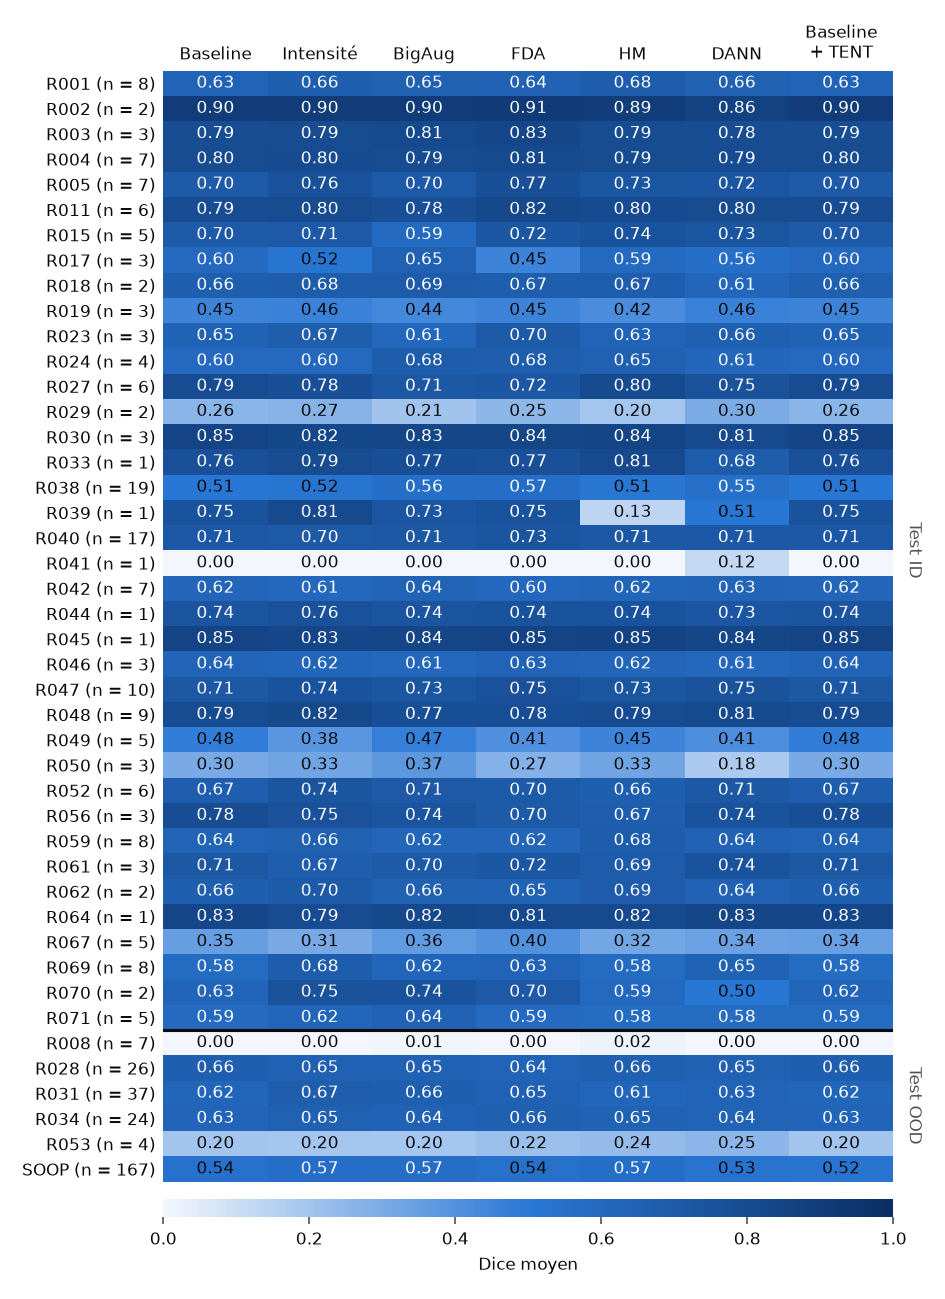
\includegraphics[width=\linewidth]{figures/rq3/rq3_dice_par_centre.png}
  \caption{Dice moyen par centre de test (ID et OOD) et par technique. HM : histogram matching.}
  \label{fig:rq3-dice-centre}
\end{figure}

\subsection{Taille des lésions}

La taille est le facteur le plus net.
Sur les 265 sujets OOD, la corrélation de Spearman entre le volume de la lésion et le Dice (modèle intensité) vaut $\rho = 0{,}53$ ($p < 10^{-4}$).
Le tableau~\ref{tab:rq3-taille} et la figure~\ref{fig:rq3-dice-taille} montrent que toutes les techniques suivent le même profil.
L'intensité gagne surtout entre 1 et 50~ml (0,50 et 0,67 contre 0,46 et 0,64 pour la baseline). BigAug gagne surtout au-dessus de 10~ml (0,68 et 0,77 contre 0,64 et 0,74).

\begin{table}[htbp]
  \centering
  \caption{Dice moyen par volume de lésion sur le test OOD (Dice ID entre parenthèses). L'adaptation continue porte sur un sous-ensemble des sujets.}
  \label{tab:rq3-taille}
  \small
  \begin{tabular}{lcccc}
    \toprule
    Technique & $< 1$~ml & 1--10~ml & 10--50~ml & $\geq 50$~ml \\
    \midrule
    Sujets OOD (ID) & 41 (34) & 86 (65) & 80 (48) & 58 (38) \\
    \midrule
    Baseline & 0,31 (0,48) & 0,46 (0,58) & 0,64 (0,71) & 0,74 (0,83) \\
    Intensité & 0,33 (0,46) & 0,50 (0,59) & 0,67 (0,74) & 0,74 (0,83) \\
    BigAug & 0,32 (0,43) & 0,48 (0,59) & 0,68 (0,75) & 0,77 (0,83) \\
    FDA & 0,30 (0,44) & 0,46 (0,61) & 0,66 (0,74) & 0,75 (0,84) \\
    Histogram matching & 0,33 (0,49) & 0,49 (0,58) & 0,66 (0,71) & 0,74 (0,83) \\
    DANN & 0,29 (0,46) & 0,45 (0,58) & 0,63 (0,73) & 0,75 (0,83) \\
    Baseline + TENT & 0,32 (0,48) & 0,46 (0,58) & 0,62 (0,71) & 0,71 (0,82) \\
    Continue (contrôlée) & 0,35 & 0,48 & 0,60 & 0,81 \\
    \bottomrule
  \end{tabular}
\end{table}

\begin{figure}[htbp]
  \centering
  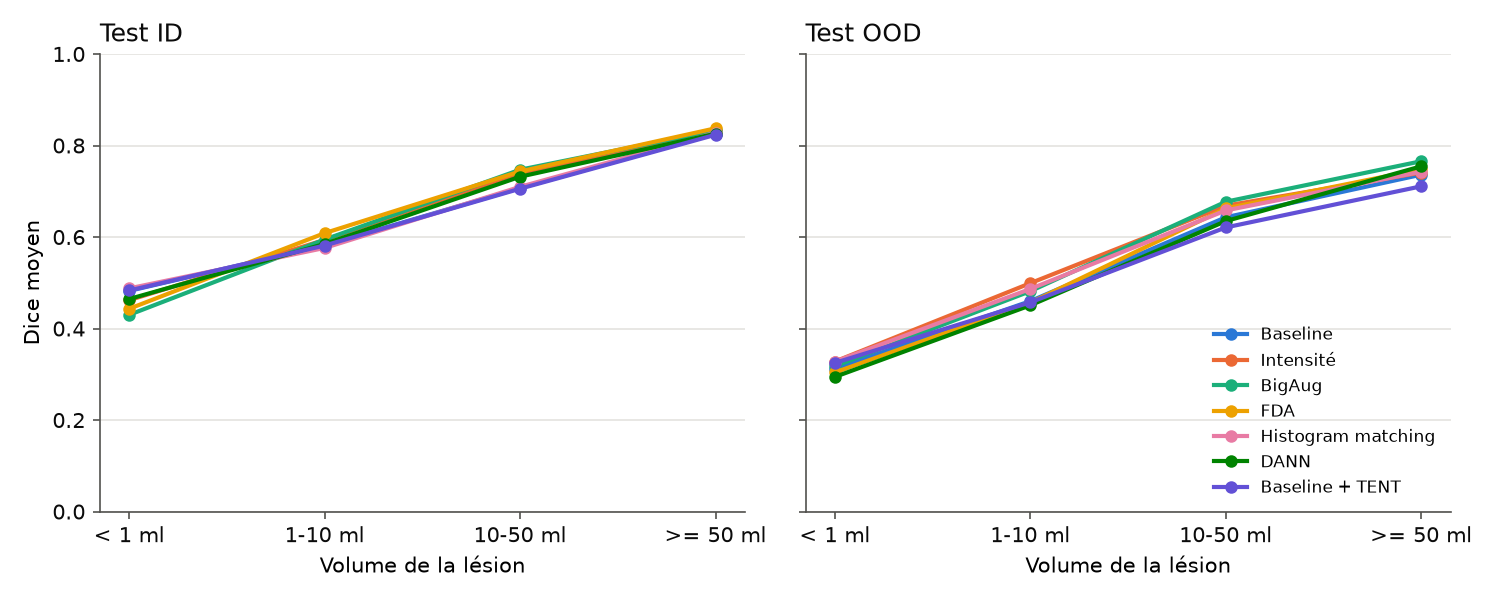
\includegraphics[width=\linewidth]{figures/rq3/rq3_dice_par_taille.png}
  \caption{Dice moyen par classe de volume de lésion, sur les tests ID (à gauche) et OOD (à droite).}
  \label{fig:rq3-dice-taille}
\end{figure}

La figure~\ref{fig:rq3-echecs-taille} reprend le test OOD en y ajoutant l'adaptation continue contrôlée.

\begin{figure}[htbp]
  \centering
  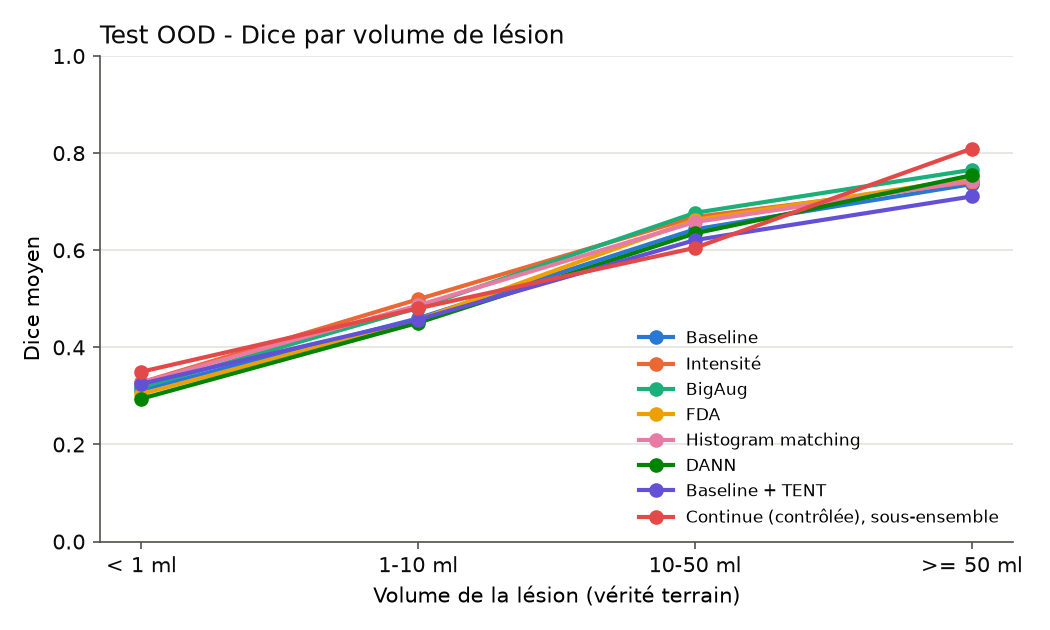
\includegraphics[width=0.8\linewidth]{figures/rq3/rq3_echecs_dice_par_taille.png}
  \caption{Dice moyen par volume de lésion sur le test OOD, avec l'adaptation continue contrôlée (sous-ensemble préquentiel).}
  \label{fig:rq3-echecs-taille}
\end{figure}

\subsection{Centre R008}

Toutes les techniques obtiennent un Dice nul ou presque sur R008. Le Dice moyen de BigAug est de 0,006 sur le centre ; un seul sujet est non nul, à 0,04 (tableau~\ref{tab:rq3-bigaug-intensite} ; moyenne arrondie à 0,01 dans le tableau~\ref{tab:rq3-centres}). Celui d'histogram matching est de 0,019, avec un seul sujet non nul, à 0,13 (tableau~\ref{tab:rq3-hm-intensite}). Le détail par sujet est dans \nolinkurl{zoom_R008_R053.csv}.
\begin{itemize}
  \item Six sujets sur sept sont imagés au premier jour après l'AVC. Leurs lésions font de 0,1 à 4,1~ml.
  \item Les lésions sont peu visibles en T1 : contraste médian de $-0{,}17$, contre $-0{,}50$ à $-0{,}98$ dans les autres centres OOD.
  \item Les intensités sont atypiques : 1,1 à 1,7~\% des voxels du cerveau dépassent $z = 3$, contre 0,003~\% en médiane chez les autres sujets OOD (\nolinkurl{contraste_lesions.csv}).
  \item Le modèle prédit de 0,4 à 33,6~ml répartis en nombreuses composantes, pour une différence du nombre de lésions de 9 à 67.
  \item À l'examen des coupes, vaisseaux, sinus et dure-mère apparaissent hyperintenses.
\end{itemize}
% Les coupes de R008 (figures/rq3/rq3_echecs_coupes_R008.png) ne sont pas incluses :
% ce sont des images ATLAS, non versionnées ; elles se régénèrent avec adaptation/analyse_echecs.py.

\emph{Hypothèse.} La séquence T1 de R008 aurait été acquise après injection de gadolinium, en phase aiguë.
La lésion n'y aurait pas encore le contraste T1 des lésions chroniques, majoritaires à l'entraînement.
Le décalage serait alors à la fois d'acquisition et de stade clinique.
Cette hypothèse reste à vérifier sur le protocole d'acquisition de R008 et sur l'écart entre la date de l'IRM et celle de l'annotation.

\subsection{Centre R053}

Le Dice moyen de R053 est de 0,20 sur quatre sujets ; un cinquième sujet a un masque vide et est exclu du Dice.
Deux lésions minuscules (0,13 et 0,015~ml) ont un Dice de 0. Les deux autres (1,5 et 2,6~ml) obtiennent 0,27 et 0,52.
Les intensités sont dans la norme (99\textsuperscript{e} centile du z-score proche de 1,8) et le contraste vaut $-0{,}50$.
L'échec s'explique par la taille des lésions, pas par un décalage d'intensité. Avec quatre sujets, la moyenne du centre est très instable.

\subsection{Distance de domaine}

La distance de Wasserstein entre histogrammes d'intensité (\nolinkurl{analysis/center_distance.py}, référence = tous les autres centres) ne prédit pas le Dice dans nos runs (\nolinkurl{spearman.csv}).
\begin{itemize}
  \item Sur les six centres OOD, $\rho$ va de $-0{,}43$ à $-0{,}03$ selon la technique ($p$ de 0,40 à 0,96). Avec la MMD, $\rho$ va de $-0{,}37$ à $-0{,}09$.
  \item Sur les 44 centres de test (ID et OOD), $\rho$ va de 0,03 à 0,12 ($p \geq 0{,}44$).
\end{itemize}
La figure~\ref{fig:rq3-distance} en donne deux contre-exemples. R053 est l'un des centres les plus proches (0,020) et l'un des pires. R031 est éloigné (0,164) et parmi les meilleurs.
Six centres offrent une puissance très faible : nous ne concluons pas à l'absence de lien, seulement qu'il n'apparaît pas ici.

\begin{figure}[htbp]
  \centering
  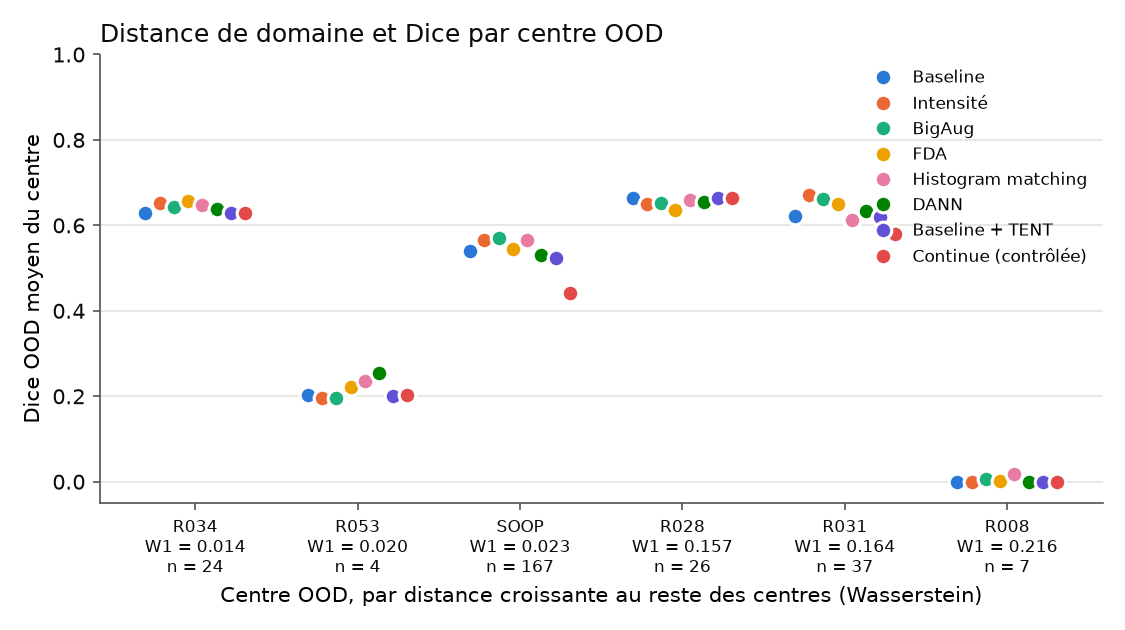
\includegraphics[width=0.8\linewidth]{figures/rq3/rq3_echecs_distance_dice.png}
  \caption{Dice OOD moyen par centre, les centres étant rangés par distance croissante au reste des centres.}
  \label{fig:rq3-distance}
\end{figure}

Au niveau des sujets, le contraste de la lésion n'est que faiblement lié au Dice ($\rho = -0{,}19$, $p = 0{,}001$). La figure~\ref{fig:rq3-contraste} montre ce nuage et place les sujets de R008 et R053.

\begin{figure}[htbp]
  \centering
  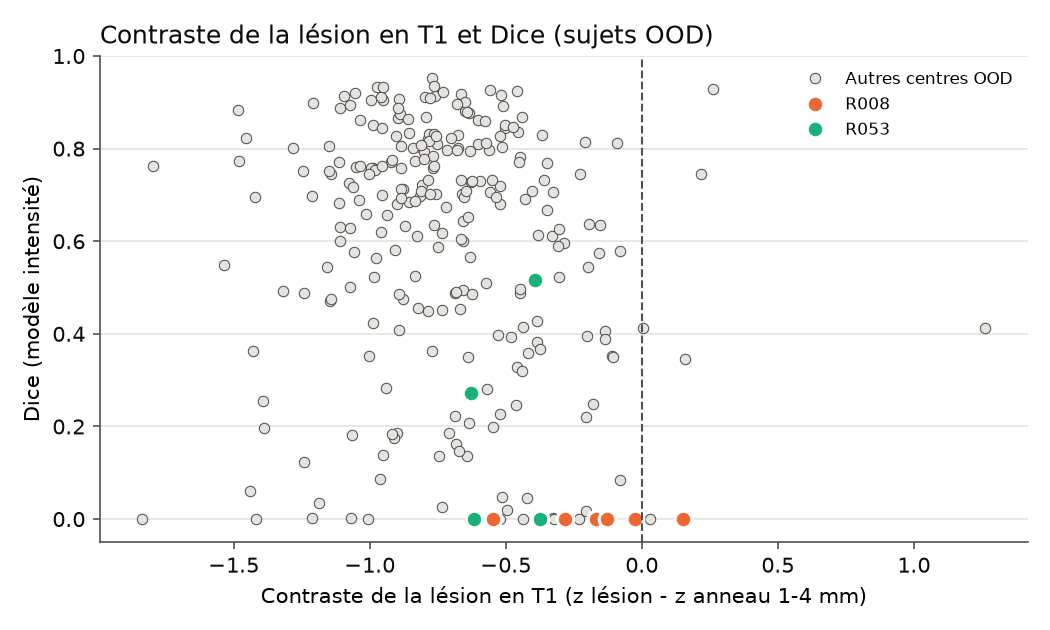
\includegraphics[width=0.8\linewidth]{figures/rq3/rq3_echecs_contraste_dice.png}
  \caption{Contraste T1 de la lésion et Dice (modèle intensité) pour les sujets OOD ; R008 et R053 sont mis en évidence.}
  \label{fig:rq3-contraste}
\end{figure}

\section{Adaptation continue contrôlée}
\label{sec:rq3-continue}

\paragraph{Protocole.}
L'expérience est réalisée par le script \nolinkurl{adaptation/continual.py}.
Ses sorties se trouvent dans le dossier \nolinkurl{adaptation/outputs/rq3/adaptation_continue/}.
Le modèle baseline reçoit les six centres OOD l'un après l'autre, par lots de quatre sujets : 28 lots, 108 sujets, au plus 24 par centre. Il n'est jamais réinitialisé.
L'évaluation est préquentielle : chaque lot est d'abord noté (Dice), puis utilisé pour l'adaptation, sans étiquettes.
Quatre stratégies sont comparées sur les mêmes lots :
\begin{itemize}
  \item \texttt{fige} : le modèle reste inchangé ;
  \item \texttt{auto\_apprentissage} : pseudo-étiquettes, tous les poids sont mis à jour ;
  \item \texttt{tent} : TENT appliqué en continu ;
  \item \texttt{controlee} : TENT dans un modèle candidat, promu seulement si trois conditions sont réunies. (1) La distance du lot dépasse un seuil calibré sur la source (0,077). (2) L'entropie baisse sur des patches neufs. (3) Le Dice sur un jeu de garde étiqueté de la source ne baisse pas de plus de 0,01. Cette stratégie rejoue aussi des exemples des centres déjà vus et des patches de la source.
\end{itemize}
L'oubli est mesuré après chaque centre, par le Dice sur 16 sujets fixes du test ID et sur les premiers sujets des centres OOD déjà vus.

\paragraph{Résultats.}
Le tableau~\ref{tab:rq3-continue} résume les quatre stratégies (\nolinkurl{resume.json}, \nolinkurl{oubli.csv}).

\begin{table}[htbp]
  \centering
  \caption{Adaptation continue sur les six centres OOD : Dice préquentiel et oubli.}
  \label{tab:rq3-continue}
  \small
  \begin{tabular}{lcccc}
    \toprule
    Stratégie & \makecell{Dice\\préquentiel} & \makecell{Dice ID\\(début $\rightarrow$ fin)} & Oubli ID & \makecell{Oubli OOD\\moyen} \\
    \midrule
    Figé & 0,528 & 0,635 $\rightarrow$ 0,635 & 0,000 & 0,000 \\
    Auto-apprentissage & 0,486 & 0,635 $\rightarrow$ 0,583 & 0,052 & 0,033 \\
    TENT continu & 0,526 & 0,635 $\rightarrow$ 0,632 & 0,002 & 0,000 \\
    Contrôlée & 0,527 & 0,635 $\rightarrow$ 0,634 & 0,001 & 0,000 \\
    \bottomrule
  \end{tabular}
\end{table}

Les décisions lot par lot sont dans \nolinkurl{decisions.csv}.
\begin{itemize}
  \item \textbf{Détection.} Un décalage est détecté sur 15 lots sur 28 : tous ceux de R008, R028 et R031, et un lot sur six de SOOP. Il n'est jamais détecté sur R034 ni R053, les centres les plus proches de la source.
  \item \textbf{Promotions.} Douze candidats sont promus : deux pour R008, six pour R028, trois pour R031 et un pour SOOP. Trois candidats de R031 sont refusés parce que leur entropie augmente.
  \item \textbf{Oubli.} La stratégie contrôlée évite l'oubli de l'auto-apprentissage (0,001 contre 0,052 sur le test ID).
  \item \textbf{Gain.} Elle n'améliore pas le Dice par rapport au modèle figé (0,527 contre 0,528).
\end{itemize}

\paragraph{Lecture du résultat.}
L'absence de gain s'explique par la nature des décalages détectés.
R028 et R031 sont déjà bien segmentés par le modèle figé (0,66 et 0,58 en préquentiel).
Sur R008, le problème tient au contraste des lésions (section~\ref{sec:rq3-echecs}), qu'une adaptation des normalisations ne peut pas créer.
Les Dice préquentiels portent sur 108 des 268 sujets OOD ; ils ne se comparent pas directement au tableau~\ref{tab:rq3-resultats}.

\section{Limites}
\label{sec:rq3-limites}

\begin{itemize}
  \item \textbf{Un seul pli et une seule graine.} Les IC traduisent la variabilité des sujets, pas celle de l'entraînement.
  \item \textbf{Reprise de DANN.} La run a été coupée à l'itération 35\,889 et reprise jusqu'à 40\,000. La reprise restaure les poids, l'optimiseur, le taux d'apprentissage, $\lambda$, la position de l'échantillonneur et les états aléatoires des processus de chargement. Le contrôle automatique a validé la première ligne reprise (itération 35\,900, taux $1{,}29 \times 10^{-4}$, $\lambda = 0{,}9771$). Seuls les masques de Dropout du classifieur de centre ne sont pas restaurés. Le meilleur modèle, à l'itération 24\,000, précède de toute façon la coupure.
  \item \textbf{Environnement de DANN.} DANN a été entraînée sur Colab avec torch 2.14.1+cu130 jusqu'à l'itération 35\,889, puis sur Kaggle avec torch 2.11.0+cu130, comme les autres runs. Les deux plateformes utilisent un GPU T4 et CUDA 13.0. Le meilleur modèle (itération 24\,000) vient de la partie Colab. La différence de version de torch peut changer les calculs numériques ; son effet n'a pas été mesuré.
  \item \textbf{Poids de DANN.} Avec un poids de 1, la première run DANN a divergé (perte totale de 10\,508 à l'itération 100 et de 33 millions à l'itération 400). Le poids de 0,1 et la LayerNorm ont été choisis pour la stabilité, sans recherche d'hyperparamètres. Un autre poids pourrait donner un autre résultat.
  \item \textbf{Validation sur des centres non vus.} Ses lésions sont plus petites que celles du test. Elle sert à choisir le checkpoint, mais son Dice (environ 0,43) n'estime pas la performance ID.
  \item \textbf{Diagnostic fp16.} La première baseline, entraînée en fp16, a produit des NaN : des patches entiers donnaient des logits NaN dès l'itération 160 à 180 environ, alors que le fp32 restait stable sur les mêmes lots. Toutes les runs ont été refaites en fp32, environ deux fois plus lentement. La couche qui déborde n'a pas été localisée.
  \item \textbf{Bug de reprise corrigé.} Dans la version du code utilisée pour les runs, la ligne de progression écrasait la file des états aléatoires sauvegardés pour la reprise. Le défaut ne concerne que les reprises, donc uniquement DANN. Il a été corrigé et couvert par un test. Le checkpoint de DANN a été réparé avant la reprise en ne gardant que les quatre derniers états, qui étaient les bons ; les poids n'ont pas changé.
  \item \textbf{Référence de la distance de domaine.} Pour chaque centre, la référence de \nolinkurl{center_distance} regroupe tous les autres centres, OOD compris, et pas seulement les centres d'entraînement du pli~0. La distance mesure donc l'écart au reste du jeu de données, pas exactement l'écart à ce que le modèle a vu.
  \item \textbf{Version du code d'histogram matching.} Cette run a utilisé une version ultérieure du code (\texttt{dbf2f28} au lieu de \texttt{7449c49}), qui ne diffère que par la correction du bug de reprise. Sans DANN ni reprise, les deux versions donnent des poids identiques (vérifié par un court entraînement sur CPU, pour la baseline et l'intensité).
  \item \textbf{Quota GPU.} Avec 30~h par semaine sur Kaggle, aucun autre pli n'a été entraîné, et l'histogram matching a été lancé après les autres techniques.
  \item \textbf{Portée de TENT et de l'adaptation continue.} Les deux ne sont évalués que sur la baseline.
\end{itemize}

\section{Conclusion}
\label{sec:rq3-conclusion}

Sur le pli~0, seule l'augmentation d'intensité améliore le Dice OOD de façon significative après correction : $+0{,}024$ [0,008 ; 0,041], $p$ Holm $= 0{,}0068$ (tableau~\ref{tab:rq3-resultats}).
BigAug atteint le même Dice OOD (0,577), mais son gain n'est pas significatif après correction ($p$ Holm $= 0{,}14$), et la comparaison directe ne sépare pas les deux techniques ($+0{,}001$ [$-0{,}010$ ; 0,012], tableau~\ref{tab:rq3-bigaug-intensite}).
Histogram matching n'est pas significatif non plus ($+0{,}017$, $p$ Holm $= 0{,}49$) ; il reste en dessous de l'intensité en Dice OOD ($-0{,}007$ [$-0{,}023$ ; 0,009]), avec un écart net sur R031 (tableau~\ref{tab:rq3-hm-intensite}).
Aucune technique ne supprime l'écart ID $-$ OOD, qui reste compris entre 0,075 et 0,104.
FDA, DANN et TENT n'améliorent pas le test OOD ; TENT le dégrade légèrement.
L'adaptation continue contrôlée évite l'oubli sans améliorer le Dice (tableau~\ref{tab:rq3-continue}).
L'analyse des échecs montre que les cas les plus difficiles tiennent aux lésions elles-mêmes, petites ou peu contrastées en T1, plutôt qu'à la distance d'intensité entre centres.
Le livrable C8 (\nolinkurl{adaptation/inference.py}) segmente un T1 et renvoie le masque et le volume de la lésion.
Le modèle retenu pour la démonstration est celui de l'intensité.
À Dice égal avec BigAug, ce choix repose d'abord sur son gain significatif après correction, ensuite sur un entraînement plus court (5,0~h contre 8,1~h).
Son F1 des lésions est supérieur à celui de BigAug (0,450 contre 0,420) mais inférieur à celui de la baseline (0,477) : ce n'est qu'un argument relatif face à BigAug.
Histogram matching a le plus faible écart absolu de volume (9,1~ml contre 10,0~ml pour l'intensité) et un F1 des lésions supérieur à celui de la baseline (0,486 contre 0,477).
Il n'a pas été retenu, car son gain en Dice n'est pas significatif et il exigerait d'harmoniser aussi chaque volume à l'inférence, avec l'histogramme de référence de R059.
Ces constats orientent la suite vers la prédiction des cas à risque, en particulier les lésions de moins de 1~ml et les AVC en phase aiguë.
